\documentclass[12pt,oneside]{book}

%%%%%%%%%%%%%%%%%%%%%%%%%%%%%%%%%%%%%%%%%%%%%%%%%%%%%%%%%%%%%%%%%%%%%%%%%%%%%%%%%%%%%%%%%%%%%%%%%%%
%                                                                                                 %
% The mathematical style of these documents follows                                               %
%                                                                                                 %
% A. Thompson and B.N. Taylor. The NIST Guide for the Use of the International System of Units.   %
%    NIST Special Publication 881, 2008.                                                          %
%                                                                                                 %
% http://www.nist.gov/pml/pubs/sp811/index.cfm                                                    %
%                                                                                                 %
%%%%%%%%%%%%%%%%%%%%%%%%%%%%%%%%%%%%%%%%%%%%%%%%%%%%%%%%%%%%%%%%%%%%%%%%%%%%%%%%%%%%%%%%%%%%%%%%%%%

% $Date: 2013-11-26 10:43:59 -0500 (Tue, 26 Nov 2013) $
% $Revision: 17538 $
% $Author: gforney $

%%%%%%%%%%%%%%%%%%%%%%%%%%%%%%%%%%%%%%%%%%%%%%%%%%%%%%%%%%%%%%%%%%%%%%%%%%%%%%%%%%%%%%%%%%%%%%%%%%%
%                                                                                                 %
% The mathematical style of these documents follows                                               %
%                                                                                                 %
% A. Thompson and B.N. Taylor. The NIST Guide for the Use of the International System of Units.   %
%    NIST Special Publication 881, 2008.                                                          %
%                                                                                                 %
% http://www.nist.gov/pml/pubs/sp811/index.cfm                                                    %
%                                                                                                 %
%%%%%%%%%%%%%%%%%%%%%%%%%%%%%%%%%%%%%%%%%%%%%%%%%%%%%%%%%%%%%%%%%%%%%%%%%%%%%%%%%%%%%%%%%%%%%%%%%%%

% Packages which force the use of better TeX coding
% Mostly from http://tex.stackexchange.com/q/19264
%%\RequirePackage[l2tabu, orthodox]{nag}
%%\usepackage{fixltx2e}
%\usepackage{isomath} % Disabled for the moment because it changes the syntax for bold and roman Greek math symbols
%%\usepackage[all,warning]{onlyamsmath}
%\usepackage{strict} % Commented out for now because it is uncommon. A copy of style.sty is in Manuals/LaTeX_Style_Files/.

\usepackage{times,mathptmx}
\usepackage[pdftex]{graphicx}
\usepackage{tabularx,ragged2e,booktabs,caption}
\usepackage{multirow}
\usepackage{pdfsync}
\usepackage{tikz}
\usepackage{pgfplots}
%\pgfplotsset{compat=1.7}
\usepackage{tocloft}
\usepackage{color}
\usepackage{amsmath}
\definecolor{linknavy}{rgb}{0,0,0.50196}
\definecolor{linkred}{rgb}{1,0,0}
\definecolor{linkblue}{rgb}{0,0,1}
\usepackage{float}
\usepackage{caption}
\usepackage{graphpap}
\usepackage{rotating}
\usepackage{graphicx}
\usepackage{geometry}
\usepackage{relsize}
\usepackage{longtable}
\usepackage{lscape}
\usepackage{amssymb}
\usepackage{makeidx} % Create index at end of document
\usepackage[nottoc,notlof,notlot]{tocbibind} % Put the bibliography and index in the ToC
\usepackage{lastpage} % Automatic last page number reference.
\usepackage[T1]{fontenc}
\usepackage{enumerate}
\usepackage{upquote}
\usepackage{moreverb}
\usepackage{xfrac}
\usepackage{cite}

\newcommand{\nopart}{\expandafter\def\csname Parent-1\endcsname{}} % To fix table of contents in pdf.
\newcommand{\ct}{\tt\small} % eventually will be deprecated due to http://www.tex.ac.uk/cgi-bin/texfaq2html?label=2letterfontcmd
\newcommand{\textct}[1]{\texttt{\small #1}}

\usepackage{tocstyle} % Fix table of contents sections from overlapping section titles
\usetocstyle{standard}
\usepackage{siunitx}
\sisetup{
    detect-all = true,
    input-decimal-markers = {.},
    input-ignore = {,},
    inter-unit-product = \ensuremath{{}\cdot{}},
    multi-part-units = repeat,
    number-unit-product = \text{~},
    per-mode = fraction,
    separate-uncertainty = true,
}

\usepackage{listings}
\usepackage{textcomp}
\definecolor{lbcolor}{rgb}{0.96,0.96,0.96}
\lstset{
    %backgroundcolor=\color{lbcolor},
    tabsize=4,
    rulecolor=,
    language=Fortran,
        basicstyle=\footnotesize\ttfamily,
        upquote=true,
        aboveskip={\baselineskip},
        belowskip={\baselineskip},
        columns=fixed,
        extendedchars=true,
        breaklines=true,
        breakatwhitespace=true,
        frame=none,
        showtabs=false,
        showspaces=false,
        showstringspaces=false,
        identifierstyle=\ttfamily,
        keywordstyle=\color[rgb]{0,0,0},
        commentstyle=\color[rgb]{0,0,0},
        stringstyle=\color[rgb]{0,0,0},
}

\usepackage[pdftex,
        colorlinks=true,
        urlcolor=linkblue,     % \href{...}{...} external (URL)
        citecolor=linkred,     % citation number colors
        linkcolor=linknavy,    % \ref{...} and \pageref{...}
        pdfproducer={pdflatex},
        pdfpagemode=UseNone,
        bookmarksopen=true,
        plainpages=false,
        verbose]{hyperref}

% The Following commented code makes the ``Draft'' watermark on each page.
%\usepackage{eso-pic}
%\usepackage{type1cm}
%\makeatletter
%   \AddToShipoutPicture{
%     \setlength{\@tempdimb}{.5\paperwidth}
%     \setlength{\@tempdimc}{.5\paperheight}
%     \setlength{\unitlength}{1pt}
%     \put(\strip@pt\@tempdimb,\strip@pt\@tempdimc){
%     \makebox(0,0){\rotatebox{45}{\textcolor[gray]{0.75}{\fontsize{8cm}\selectfont{RC6}}}}}
% }
%\makeatother

\setlength{\textwidth}{6.5in}
\setlength{\textheight}{9.0in}
\setlength{\topmargin}{0.in}
\setlength{\headheight}{0.pt}
\setlength{\headsep}{0.in}
\setlength{\parindent}{0.25in}
\setlength{\oddsidemargin}{0.0in}
\setlength{\evensidemargin}{0.0in}
\setlength{\leftmargini}{\parindent} % Controls the indenting of the "bullets" in a list
\setlength{\cftsecnumwidth}{0.45in}
\setlength{\cftsubsecnumwidth}{0.5in}
\setlength{\cftfignumwidth}{0.45in}
\setlength{\cfttabnumwidth}{0.45in}

\newcommand{\titlesigs}
{
\small
\flushright{U.S. Department of Commerce \\
{\em Penny Pritzker, Secretary} \\
\hspace{1in} \\
National Institute of Standards and Technology \\
{\em Willie May, Under Secretary of Commerce for Standards and Technology and Acting Director} }
}

% commands to use for "official" cover and title pages
% see smokeview verification guide to see how they are used

\newcommand{\headerA}[1]{
\flushright{
\fontsize{20}{24}\selectfont
\bf{NIST Special Publication #1}}
}

\newcommand{\headerB}[1]{
\flushright{
\fontsize{28}{33.6}\selectfont
\bf{#1}
}
}

\newcommand{\headerC}[1]{
\vspace{.5in}
\flushright{\fontsize{14}{16.8}\selectfont
#1}
}

\frenchspacing

\newcommand{\dod}[2]{\frac{\partial #1}{\partial #2}}
\newcommand{\DoD}[2]{\frac{\mathrm{D} #1}{\mathrm{D} #2}}
\newcommand{\dsods}[2]{\frac{\partial^2 #1}{\partial #2^2}}
\renewcommand{\d}{\,\mathrm{d}}
\newcommand{\dx}{\delta x}
\newcommand{\dy}{\delta y}
\newcommand{\dz}{\delta z}
\newcommand{\degF}{$^\circ$F}
\newcommand{\degC}{$^\circ$C}
\newcommand{\x}{x}
\newcommand{\y}{y}
\newcommand{\z}{z}
\newcommand{\dt}{\delta t}
\newcommand{\dn}{\delta n}
\newcommand{\cH}{H}
\newcommand{\hu}{u}
\newcommand{\hv}{v}
\newcommand{\hw}{w}
\newcommand{\la}{\lambda}
\newcommand{\bO}{{\Omega}}
\newcommand{\bo}{{\mathbf{\omega}}}
\newcommand{\btau}{\mathbf{\tau}}
\newcommand{\bdelta}{{\mathbf{\delta}}}
\newcommand{\sumyw}{\sum (Y_\alpha/W_\alpha)}
\newcommand{\oW}{\overline{W}}
\newcommand{\om}{\ensuremath{\omega}}
\newcommand{\omx}{\omega_x}
\newcommand{\omy}{\omega_y}
\newcommand{\omz}{\omega_z}
\newcommand{\erf}{\hbox{erf}}
\newcommand{\erfc}{\hbox{erfc}}
\newcommand{\bF}{{\mathbf{F}}}
\newcommand{\bG}{{\mathbf{G}}}
\newcommand{\bof}{{\mathbf{f}}}
\newcommand{\bq}{{\mathbf{q}}}
\newcommand{\br}{{\mathbf{r}}}
\newcommand{\bu}{{\mathbf{u}}}
\newcommand{\bx}{{\mathbf{x}}}
\newcommand{\bk}{{\mathbf{k}}}
\newcommand{\bv}{{\mathbf{v}}}
\newcommand{\bg}{{\mathbf{g}}}
\newcommand{\bn}{{\mathbf{n}}}
\newcommand{\bS}{{\mathbf{S}}}
\newcommand{\bW}{\overline{W}}
\newcommand{\dS}{d{\mathbf{S}}}
\newcommand{\bs}{{\mathbf{s}}}
\newcommand{\bI}{{\mathbf{I}}}
\newcommand{\hp}{H}
\newcommand{\trho}{\tilde{\rho}}
\newcommand{\dph}{{\delta\phi}}
\newcommand{\dth}{{\delta\theta}}
\newcommand{\tp}{\tilde{p}}
\newcommand{\bp}{\overline{p}}
\newcommand{\dQ}{\dot{Q}}
\newcommand{\dq}{\dot{q}}
\newcommand{\dbq}{\dot{\mathbf{q}}}
\newcommand{\dm}{\dot{m}}
\newcommand{\ha}{\frac{1}{2}}
\newcommand{\ft}{\frac{4}{3}}
\newcommand{\ot}{\frac{1}{3}}
\newcommand{\fofi}{\frac{4}{5}}
\newcommand{\of}{\frac{1}{4}}
\newcommand{\twth}{\frac{2}{3}}
\newcommand{\R}{R}
\newcommand{\be}{\begin{equation}}
\newcommand{\ee}{\end{equation}}
\newcommand{\RE}{\hbox{Re}}
\newcommand{\LE}{\hbox{Le}}
\newcommand{\PR}{\hbox{Pr}}
\newcommand{\PE}{\hbox{Pe}}
\newcommand{\NU}{\hbox{Nu}}
\newcommand{\SC}{\hbox{Sc}}
\newcommand{\SH}{\hbox{Sh}}
\newcommand{\WE}{\hbox{We}}
\newcommand{\COTWO}{\text{\tiny \hbox{CO}$_2$}}
\newcommand{\HTWOO}{\text{\tiny \hbox{H}$_2$\hbox{O}}}
\newcommand{\OTWO}{\text{\tiny \hbox{O}$_2$}}
\newcommand{\NTWO}{\text{\tiny \hbox{N}$_2$}}
\newcommand{\CO}{\text{\tiny \hbox{CO}}}
\newcommand{\F}{\text{\tiny \hbox{F}}}
\newcommand{\C}{\text{\tiny \hbox{C}}}
\newcommand{\Hy}{\text{\tiny \hbox{H}}}
\newcommand{\So}{\text{\tiny \hbox{S}}}
\newcommand{\M}{\text{\tiny \hbox{M}}}
\newcommand{\xx}{\text{\tiny \hbox{x}}}
\newcommand{\yy}{\text{\tiny \hbox{y}}}
\newcommand{\zz}{\text{\tiny \hbox{z}}}
\newcommand{\smvlines}{115~000}

\newcommand{\calH}{\mathcal{H}}
\newcommand{\calR}{\mathcal{R}}

\newcommand{\dif}{\mathrm{d}}
\newcommand{\Div}{\nabla\cdot}
\newcommand{\D}{\mbox{D}}
\newcommand{\mhalf}{\mbox{$\frac{1}{2}$}}
\newcommand{\thalf}{\mbox{\tiny $\frac{1}{2}$}}
\newcommand{\tripleprime}{{\prime\prime\prime}}
\newcommand{\ppp}{{\prime\prime\prime}}
\newcommand{\pp}{{\prime\prime}}

\newcommand{\superscript}[1]{\ensuremath{^{\textrm{\tiny #1}}}}
\newcommand{\subscript}[1]{\ensuremath{_{\textrm{\tiny #1}}}}

\newcommand{\rb}[1]{\raisebox{1.5ex}[0pt]{#1}}

\newcommand{\Ra}{$\Rightarrow$}
\newcommand{\hhref}[1]{\href{#1}{{\tt #1}}}
\newcommand{\fdsinput}[1]{{\scriptsize\verbatiminput{../../Verification/Visualization/#1}}}

\definecolor{AQUAMARINE}{rgb}{0.49804,1.00000,0.83137}
\definecolor{ANTIQUE WHITE}{rgb}{0.98039,0.92157,0.84314}
\definecolor{BEIGE}{rgb}{0.96078,0.96078,0.86275}
\definecolor{BLACK}{rgb}{0.00000,0.00000,0.00000}
\definecolor{BLUE}{rgb}{0.00000,0.00000,1.00000}
\definecolor{BLUE VIOLET}{rgb}{0.54118,0.16863,0.88627}
\definecolor{BRICK}{rgb}{0.61176,0.40000,0.12157}
\definecolor{BROWN}{rgb}{0.64706,0.16471,0.16471}
\definecolor{BURNT SIENNA}{rgb}{0.54118,0.21176,0.05882}
\definecolor{BURNT UMBER}{rgb}{0.54118,0.20000,0.14118}
\definecolor{CADET BLUE}{rgb}{0.37255,0.61961,0.62745}
\definecolor{CHOCOLATE}{rgb}{0.82353,0.41176,0.11765}
\definecolor{COBALT}{rgb}{0.23922,0.34902,0.67059}
\definecolor{CORAL}{rgb}{1.00000,0.49804,0.31373}
\definecolor{CYAN}{rgb}{0.00000,1.00000,1.00000}
\definecolor{DIMGRAY }{rgb}{0.41176,0.41176,0.41176}
\definecolor{EMERALD GREEN}{rgb}{0.00000,0.78824,0.34118}
\definecolor{FIREBRICK}{rgb}{0.69804,0.13333,0.13333}
\definecolor{FLESH}{rgb}{1.00000,0.49020,0.25098}
\definecolor{FOREST GREEN}{rgb}{0.13333,0.54510,0.13333}
\definecolor{GOLD }{rgb}{1.00000,0.84314,0.00000}
\definecolor{GOLDENROD}{rgb}{0.85490,0.64706,0.12549}
\definecolor{GRAY}{rgb}{0.50196,0.50196,0.50196}
\definecolor{GREEN}{rgb}{0.00000,1.00000,0.00000}
\definecolor{GREEN YELLOW}{rgb}{0.67843,1.00000,0.18431}
\definecolor{HONEYDEW}{rgb}{0.94118,1.00000,0.94118}
\definecolor{HOT PINK}{rgb}{1.00000,0.41176,0.70588}
\definecolor{INDIAN RED}{rgb}{0.80392,0.36078,0.36078}
\definecolor{INDIGO}{rgb}{0.29412,0.00000,0.50980}
\definecolor{IVORY}{rgb}{1.00000,1.00000,0.94118}
\definecolor{IVORY BLACK}{rgb}{0.16078,0.14118,0.12941}
\definecolor{KELLY GREEN}{rgb}{0.00000,0.50196,0.00000}
\definecolor{KHAKI}{rgb}{0.94118,0.90196,0.54902}
\definecolor{LAVENDER}{rgb}{0.90196,0.90196,0.98039}
\definecolor{LIME GREEN}{rgb}{0.19608,0.80392,0.19608}
\definecolor{MAGENTA}{rgb}{1.00000,0.00000,1.00000}
\definecolor{MAROON}{rgb}{0.50196,0.00000,0.00000}
\definecolor{MELON}{rgb}{0.89020,0.65882,0.41176}
\definecolor{MIDNIGHT BLUE}{rgb}{0.09804,0.09804,0.43922}
\definecolor{MINT}{rgb}{0.74118,0.98824,0.78824}
\definecolor{NAVY}{rgb}{0.00000,0.00000,0.50196}
\definecolor{OLIVE}{rgb}{0.50196,0.50196,0.00000}
\definecolor{OLIVE DRAB}{rgb}{0.41961,0.55686,0.13725}
\definecolor{ORANGE}{rgb}{1.00000,0.50196,0.00000}
\definecolor{ORANGE RED}{rgb}{1.00000,0.27059,0.00000}
\definecolor{ORCHID}{rgb}{0.85490,0.43922,0.83922}
\definecolor{PINK}{rgb}{1.00000,0.75294,0.79608}
\definecolor{POWDER BLUE}{rgb}{0.69020,0.87843,0.90196}
\definecolor{PURPLE}{rgb}{0.50196,0.00000,0.50196}
\definecolor{RASPBERRY}{rgb}{0.52941,0.14902,0.34118}
\definecolor{RED}{rgb}{1.00000,0.00000,0.00000}
\definecolor{ROYAL BLUE}{rgb}{0.25490,0.41176,0.88235}
\definecolor{SALMON}{rgb}{0.98039,0.50196,0.44706}
\definecolor{SANDY BROWN}{rgb}{0.95686,0.64314,0.37647}
\definecolor{SEA GREEN}{rgb}{0.32941,1.00000,0.62353}
\definecolor{SEPIA}{rgb}{0.36863,0.14902,0.07059}
\definecolor{SIENNA}{rgb}{0.62745,0.32157,0.17647}
\definecolor{SILVER}{rgb}{0.75294,0.75294,0.75294}
\definecolor{SKY BLUE}{rgb}{0.52941,0.80784,0.92157}
\definecolor{SLATEBLUE}{rgb}{0.41569,0.35294,0.80392}
\definecolor{SLATE GRAY}{rgb}{0.43922,0.50196,0.56471}
\definecolor{SPRING GREEN}{rgb}{0.00000,1.00000,0.49804}
\definecolor{STEEL BLUE}{rgb}{0.27451,0.50980,0.70588}
\definecolor{TAN}{rgb}{0.82353,0.70588,0.54902}
\definecolor{TEAL}{rgb}{0.00000,0.50196,0.50196}
\definecolor{THISTLE}{rgb}{0.84706,0.74902,0.84706}
\definecolor{TOMATO }{rgb}{1.00000,0.38824,0.27843}
\definecolor{TURQUOISE}{rgb}{0.25098,0.87843,0.81569}
\definecolor{VIOLET}{rgb}{0.93333,0.50980,0.93333}
\definecolor{VIOLET RED}{rgb}{0.81569,0.12549,0.56471}
\definecolor{WHITE}{rgb}{1.00000,1.00000,1.00000}
\definecolor{YELLOW}{rgb}{1.00000,1.00000,0.00000}

\pgfplotsset{
	colormap={blackwhite}{[5pt]
		rgb255(0pt)=(0,0,255); 
		rgb255(100pt)=(0,255,255); 
		rgb255(200pt)=(0,255,0); 
		rgb255(300pt)=(255,255,0); 
		rgb255(400pt)=(255,0,0)
	},
} % defines smokeview colorbar


\floatstyle{boxed}
\newfloat{notebox}{H}{lon}
\newfloat{warning}{H}{low}

% Set default longtable alignment
\setlength\LTleft{0pt}
\setlength\LTright{0pt}


% Rename chapter headings
\renewcommand{\chaptername}{Section}
\renewcommand{\bibname}{References}

% Math shortcuts
\renewcommand{\sb}[1]{_\mathrm{#1}}
\renewcommand{\C}{\mbox{C}}
\renewcommand{\H}{\mbox{H}}
\renewcommand{\O}{\mbox{O}}
\newcommand{\N}{\mbox{N}}

\begin{document}

\bibliographystyle{unsrt}
\pagestyle{empty}

\begin{minipage}[t][9in][s]{6.25in}

\begin{flushright}
\fontsize{20}{24}\selectfont
\bf{NIST Technical Note 1838}
\end{flushright}

\headerB{
Simulation of an Attic Fire \\
in a Wood Frame Residential \\
Structure - Chicago, IL \\
}

\normalsize

\headerC{
{
\flushright{
Craig G. Weinschenk \\
Daniel Madrzykowski \\
Kristopher J. Overholt \\

\vspace*{2\baselineskip}

\begingroup
\hypersetup{urlcolor=black}
\href{http://dx.doi.org/10.6028/NIST.TN.1838}{http://dx.doi.org/10.6028/NIST.TN.1838}
\endgroup
}

\vfill

\flushright{


\includegraphics[width=2.in]{../../../Bibliography/nistident_flright_vec} \\[.3in]
}
}
}

\end{minipage}

\newpage
\hspace{5in}
\newpage

\frontmatter

\pagenumbering{roman}

\begin{minipage}[t][9in][s]{6.25in}

\begin{flushright}
\fontsize{20}{24}\selectfont
\bf{NIST Technical Note 1838}
\end{flushright}

\headerB{
Simulation of an Attic Fire \\
in a Wood Frame Residential \\
Structure - Chicago, IL \\
}

\headerC{
\flushright{
Craig G. Weinschenk \\
Daniel Madrzykowski \\
Kristopher J. Overholt \\
{\em Fire Research Division \\
Engineering Laboratory} \\

\vspace*{2\baselineskip}

\begingroup
\hypersetup{urlcolor=black}
\href{http://dx.doi.org/10.6028/NIST.TN.1838}{http://dx.doi.org/10.6028/NIST.TN.1838} \\
\endgroup

\vspace*{2\baselineskip}

August 2014}}

\vfill

\flushright{
\includegraphics[width=1in]{../../../Bibliography/doc} }

\titlesigs

\end{minipage}

\newpage

\begin{minipage}[t][9in][s]{6.25in}

\flushright{Certain commercial entities, equipment, or materials may be identified in this \\
document in order to describe an experimental procedure or concept adequately. \\
Such identification is not intended to imply recommendation or endorsement by the \\
National Institute of Standards and Technology, nor is it intended to imply that the \\
entities, materials, or equipment are necessarily the best available for the purpose. \\
}

\vspace{3in}

\large
\flushright{\bf National Institute of Standards and Technology Technical Note 1838 \\
Natl.~Inst.~Stand.~Technol.~Tech.~Note~1838, \pageref{LastPage} pages (August 2014) \\
% http://dx.doi.org/10.6028/NIST.TN.1838 \\
CODEN: NTNOEF }

\vfill

\hspace{1in}

\end{minipage}

\newpage

\frontmatter

\pagestyle{plain}
\pagenumbering{roman}

\cleardoublepage
\phantomsection
\addcontentsline{toc}{chapter}{Contents}
\tableofcontents

\cleardoublepage
\phantomsection
\addcontentsline{toc}{chapter}{List of Figures}
\listoffigures

\cleardoublepage
\phantomsection
\addcontentsline{toc}{chapter}{List of Tables}
\listoftables

\chapter{List of Acronyms}

\begin{tabbing}
\hspace{1.5in} \= \\
BC \> Battalion Chief \\
E \> Engine \\
FDS \> Fire Dynamics Simulator \\
HGL \> Hot Gas Layer \\
HRR \> Heat Release Rate \\
HRRPUA \> Heat Release Rate per Unit Area \\
IC \> Incident Command \\
LODD \> Line of Duty Death \\
NIOSH \> National Institute for Occupational Safety and Health \\
NIST \> National Institute of Standards and Technology \\
SFPE \> Society of Fire Protection Engineers \\
SQ \> Squad \\
TL \> Tower Ladder \\
\end{tabbing}

\chapter{List of Symbols}

\begin{tabbing}
\hspace{1.5in} \= \\
ft \> foot \\
m \> meter \\
min \> minute \\
Pa \> Pascal \\
psi \> pound per square inch \\
s \> second \\
W \> Watt \\
$k$ \> thermal conductivity \\
$\rho$ \> density \\
$c_{p}$ \> specific heat \\
\end{tabbing}

\mainmatter

\chapter*{\centering Abstract}
The Fire Dynamics Simulator (FDS) fire model, which is developed and maintained by the National Institute of Standards and Technology (NIST), was used to provide insight into the dynamics of a fire that occurred on November 2, 2012, within a 2~\sfrac{1}{2}~story, single family structure in Chicago, IL, that resulted in the death of the captain of a fire department. The inputs for the FDS simulations are documented in this report and are based on the fire scenario, including the building geometry, interior furnishings, and ventilation conditions. The fire started in the attic and spread down through an opening into the enclosed porch on the rear of the structure. This resulted in ventilation limited (fuel rich) fire conditions in the attic and rear porch areas. The spread of fire and hot gases into the second floor of the structure was limited by a closed steel-faced, wood-framed door. After exposure to the elevated temperatures and pressure from the fire in the porch area, the wood frame of the door decomposed, the steel faces of the door failed, and the door collapsed inward. The door failure resulted in the establishment of a flow path between the higher pressure and higher temperature conditions in the enclosed porch and the lower pressure and lower temperature conditions in the hallway and kitchen areas of the second floor. The temperature of the gases that flowed into the hallway exceeded 260~$^{\circ}$C (500~$^{\circ}$F) at a height of 1.86~m (6~ft). Unfortunately, a captain and firefighter were advancing a hose line in the hallway near the door at the time of the door failure. It appears that the captain was likely overcome by the rapid change in conditions before he could exit to the safety of the kitchen area. After a Mayday call, the captain was rescued from the structure, but later succumbed to his injuries.

\chapter{Introduction}
Part of the function of the Fire Research Division at the National Institute of Standards and Technology (NIST) is to develop and apply technology, measurements, and standards to improve the understanding of the behavior, prevention, and control of fires to enhance fire fighting operations and equipment, fire suppression, fire investigations, and disaster response. NIST has previously used the Fire Dynamics Simulator (FDS) fire model to provide insight into the fire development and thermal conditions of fires that have resulted in line of duty deaths (LODDs)~\cite{Madrzykowski:1,Iowa,Texas,Bryner:Charleston,barowy:texas}. The objective of these studies has been to improve the safety and effectiveness of firefighters.

On November 2, 2012, a fire in a 2~\sfrac{1}{2}~story wood frame residential structure claimed the life of a captain of the Chicago Fire Department. NIST examined the fire dynamics of this incident at the request of NIOSH and the Chicago Fire Department. Computer simulations of the fire incident were conducted using the NIST Fire Dynamics Simulator~\cite{FDS_Users_Guide} and Smokeview~\cite{Smokeview_Users_Guide}  software to provide insight into the fire development and thermal conditions that likely existed in the residence during the fire. The specific objectives of the simulations detailed in this report are: 
\begin{enumerate}
\item To examine the effect of the flow path (including temperature, pressure, and fire conditions) in this multi-story residential structure using physics-based calculations.
\item To provide visualizations of the fire behavior that are representative of the conditions that members of the Chicago Fire Department likely experienced during the course of their interior operations.
\end{enumerate}
This document describes the input and the results of the FDS (version 6.0.0) simulations. The simulations were developed using a combination of knowledge of the fire scenario and appropriate engineering approximations and assumptions. Analysis of the simulation results focuses on the hazardous conditions that developed following the development of a flow path inside of the structure. This document is organized as follows: Section~\ref{fire_sum} provides a summary of the fire incident, Section~\ref{model} describes the relevant model input parameters and assumptions that were used to develop the simulations, Section~\ref{results} presents the simulation results, and Section~\ref{discussion} discusses the simulation results as they relate to firefighter safety and effectiveness. 


\chapter{Summary of the Fire Incident}
\label{fire_sum}
The account of events for this incident was documented by the National Institute for Occupational Safety and Health (NIOSH) Fire Fighter Fatality Investigation and Prevention Program Report \#F2012-28~\cite{NIOSH:Bowyer}. For the purpose of this analysis, the details regarding the timeline are considered to be approximate values. The following narrative of the incident was extracted from the NIOSH incident report~\cite{NIOSH:Bowyer}:
\begin{quote}
On November 2, 2012, a 54-year-old male career captain sustained injuries at a 2-1/2 story apartment building fire then died at the hospital. At 1716 hours, dispatch called a ``Still'' alarm\footnote{The department defines a ``Still'' alarm to be two engine companies, two truck companies, and a battalion chief.} for smoke in the area. Battalion Chief (BC) 19 was the first to leave the station that was just blocks away. He approached the fire structure by driving behind it then around to the front arriving on scene at 1717 hours. He reported a working fire with heavy smoke coming from the rear and front of the structure's attic. Per fire department standard operating procedures, dispatch initiated a RIT response\footnote{The department defines a rapid intervention team (RIT) response to be one truck company, one battalion chief, one advanced life support (ALS) ambulance, and one emergency medical services (EMS) field officer.}. At 1718 hours, E123 arrived on scene and BC19 was on scene and had assumed incident command (IC). The IC spoke with one of the occupants who stated everyone was out. The IC made entry through the front door to the stairwell to survey the interior of the 2\textsuperscript{nd} floor. He noticed only a light haze throughout and glow around the [rear] door to the covered porch. The IC came back to the front door and met the E123 captain and a firefighter. They had stretched a [hose] load which is 100 feet of 2\sfrac{1}{2}-inch, a gated wye, and 150 feet of 1\sfrac{3}{4}-inch hoseline to go to the 2\textsuperscript{nd} floor, which is a standard department hose lay for this type occupancy. At 1720 hours, E49, T33, and TL39 arrived on scene.

The IC made entry to the 1\textsuperscript{st} floor apartment and worked his way to [the rear of the structure]. He opened the [interior door opening into the rear foyer on the back side of the house] and noticed heavy fire in the covered porch and rear stairwell area. At 1721 hours, the [E123 captain] and firefighter were on the 2\textsuperscript{nd} floor where they flaked out, charged, and began advancing the hoseline to the rear door of the apartment. The E49 crew had stretched a 2\sfrac{1}{2}-inch hoseline [to the rear of the structure]. The T33 crew set a ground ladder on [the left side of the structure] and TL39 set the aerial to the roof about a third of the way back on [the left side]. A TL39 firefighter went to [the rear of the structure] to check doors. He first went to the basement door which he was unable to force open. Then, he went to the first floor exterior enclosed porch door which was unlocked and he opened it up. He stated that he noticed fire light-up in the stairwell. He kicked in the locked door [that connects the 1\textsuperscript{st} floor rear porch to the rear foyer], [proceeded] to walk in, saw no fire then backed out.

At 1723 hours, the IC radioed the [E123 captain] that there was heavy fire in the covered porch and attic area and that E49 was going to put water on the fire, around the [rear] attic window, but there was no acknowledgment from the [captain]. E49 proceeded to put water on the [rear of the structure]. The IC returned out front to the command post and donned his turnout gear. The lieutenant from TL39, the lieutenant and 2 firefighters from SQ5, and a E123 firefighter/paramedic (FF/PM) were near the kitchen area on the 2\textsuperscript{nd} floor when they heard a loud commotion. The FF/PM heard the [E123 captain] yell ``get out of here.'' The FF/PM had no radio and he couldn't locate the [captain's] radio so he yelled Mayday as he tried to get the [captain] and other crew member untangled. The TL39 Lieutenant and SQ5 fire fighters heard the FF/PM's verbal Mayday and the SQ5 Lieutenant tried to transmit a Mayday over heavy radio traffic.

At 1727 hours, the TL39 crew had just completed the first hole in the roof about midway on [the right side] roof with minimal fire showing, when they heard the Mayday. The IC verified that a firefighter was down, called a Mayday, and requested a 2-11 Assignment\footnote{The department defines a 2-11 alarm as a second alarm upgrade. The response is four engines, two trucks, one tower ladder, two battalion chiefs, one deputy district chief, one air mask service bottle truck, and a media affairs unit.}. Dispatch initiated a 2-11 alarm. SQ5 and other members on the 2\textsuperscript{nd} floor grabbed the [E123 captain] and got him down the stairs. The TL39 crew, with assistance from a T33 and SQ5 firefighter, had just completed a second hole on [the right side] of the roof about a third of the way back when conditions worsened. At 1729 hours, the roof ventilation crew was back in the aerial basket when they noticed the [captain] being brought out to the front yard. The [captain] was nonresponsive in the front yard and CPR was successfully performed. The IC met the A19 crew and escorted them to the [E123 captain]. The revived [captain] was responsive and talking to the paramedics as he was loaded into the ambulance. At 1738 hours, the [captain] was transported to the local hospital where he had complications during airway management and died.
\end{quote}

\noindent Table~\ref{tab:fire_info} shows an overview of the timeline of events. A plan view of the structure and the location where the captain collapsed are shown in Fig.~\ref{fig:simp_geom}, and more details of the fire development are provided in the following sections.

\begin{table}
\centering
\captionof{table}[Abridged NIOSH approximate fire event timeline]{Abridged NIOSH approximate fire event timeline~\cite{NIOSH:Bowyer}}\label{tab:fire_info}
\begin{tabular}{cl}
\toprule[1.5pt]
Incident Time              &  Fire Behavior / Fireground Operation                                                                                                    \\
{[hh:mm:ss]}               &                                                                                                                                          \\
\midrule
\multirow{2}{*}{17:15:00}  &  \multirow{2}{*}{\parbox{10cm} {Reported working fire with heavy smoke coming from the front and rear of the structure's attic.}}        \\ 
                           &                                                                                                                                          \\[.25cm] %blank rows exist for wrapping text. # of blanks is 1 less than number of rows
\multirow{2}{*}{17:16:00}  &   \multirow{2}{*}{\parbox{10cm} {Dispatch for a ``Still'' alarm - two engine companies, two truck companies, and a battalion chief.}}    \\
                           &                                                                                                                                          \\[.25cm]
\multirow{2}{*}{17:20:00}  &  \multirow{2}{*}{\parbox{10cm} {Attic windows break - heavy smoke out of front attic window and heavy smoke and fire out of rear.}}      \\
                           &                                                                                                                                          \\[.25cm] 
17:21:00                   &  E123 captain and firefighter on second floor with 1\sfrac{3}{4}-inch hoseline.                                                          \\[.25cm]
17:21:30                   &  First floor exterior porch door opened.                                                                                                 \\[.25cm]
\multirow{2}{*}{17:23:00}  &  \multirow{2}{*}{\parbox{10cm} {Heavy fire report in rear stairwell and enclosed porch. No response from E123 captain or firefighter.}}  \\
                           &                                                                                                                                          \\[.25cm]
17:24:00                   &   Water applied to attic from the rear exterior position.                                                                                \\[.25cm]
17:25:00                   &   SQ5 makes entry through front of structure.                                                                                            \\[.25cm]
17:27:00                   &   After hearing a Mayday call from SQ5, IC calls a Mayday.                                                                               \\[.25cm]
17:29:00                   &   E123 captain carried out of structure.                                                                                                 \\
\bottomrule[1.25pt]
\end{tabular}\par
\end{table}
 

\chapter{Model Description}
\label{model}
Fire Dynamics Simulator~\cite{FDS_Users_Guide} is a computational fluid dynamics (CFD) model that solves a form of the Navier-Stokes equations appropriate for low-speed, thermally driven flow with an emphasis on smoke and heat transport from fires.  Within a CFD model, the room or building is divided into small three-dimensional rectangular control volumes or computational cells.  The cells are contained together within one larger volume known as a computational domain.  The CFD model computes the density, velocity, temperature, pressure, and species concentration of the gas in each cell.  Based on the laws of conservation of mass, momentum,  and energy, the model tracks the generation and movement of fire gasses. One of the most important advantages of FDS is that it is  mathematically verified~\cite{FDS_Verification_Guide} and validated against fire test data to ensure that it provides the expected results, given sufficient input data~\cite{FDS_Validation_Guide}. A complete description of the FDS model is provided in the FDS Technical Reference Guide~\cite{FDS_Math_Guide}.

Smokeview is a software tool designed to visualize simulation results from FDS~\cite{Smokeview_Users_Guide}. Smokeview visualizes smoke and other attributes of the fire simulation using traditional scientific methods such as displaying tracer particle flow, two dimensional (2D) or three dimensional (3D) shaded contours of gas flow data such as temperature and flow vectors showing flow direction and magnitude. Smokeview allows the fire and fire movement to be visualized. This is done by displaying a series of partially transparent planes where the transparencies in each plane (at each grid node) are determined from soot densities computed by FDS. Smokeview also visualizes static data at particular times using 2D or 3D contours of data such as temperature and flow vectors showing flow direction and magnitude.

Input data from various sources must be collected and documented to simulate a fire using FDS or any other fire model. For the simulation results presented in this document, information was obtained from two primary sources. The following information was gathered from the fire scene: the geometry of the building and the compartments being modeled, the size and location of exterior and interior ventilation openings, and documentation of fire damage to the building. The following information was gathered from witnesses, first responders, reports, and recorded media such as fire ground radios or videos: information on the timing of the fire development, the sequence and approximate timing of ventilation openings to the outside, and weather conditions at the time of the fire. 

The analysis of the simulation results is focused on the interior conditions on the second floor before and after the interior door failure. Based on the goals of the analysis and the information collected, several engineering approximations were made. For example, the fire exhibited signs of under-ventilated conditions when firefighters arrived~\cite{NIOSH:Bowyer}; however, the exact ignition time, fire growth rate, and heat release rate (HRR) of the fire were not known. The ignition time and growth rate were estimated to reduce the amount of required calculation time while adhering to documented observations. The HRR of the fire was estimated using documentation of the potential fuel load within the structure.

In reality, the quantities associated with these input parameters are not fixed values; rather, a model input parameter can be thought of as a point estimate from a distribution of possible input parameters with some associated amount of uncertainty. Any change in an input parameter (such as the HRR) for a given scenario would result in a change in the output quantity (such as the hot gas layer (HGL) temperature). For example, according to the McCaffrey, Quintiere, and Harkleroad~\cite{SFPE:Walton} empirical correlation, the HGL temperature in a well-ventilated compartment fire is proportional to the HRR raised to the two-thirds power. Following this relationship, a 7.5~\% increase in the HRR would result in a 5~\% increase in the HGL temperature~\cite{NUREG_1824_Sup_1}. More detailed discussion on the propagation of parameter uncertainty in fire models is available in NUREG-1824 Supplement~1~\cite{NUREG_1824_Sup_1}. The following subsections describe the inputs that were used to develop the simulation, including any approximations or assumptions that were made.

\section{Geometry}
\label{geom}
The structure involved in this fire incident was a 2~\sfrac{1}{2}~story residential building with balloon frame construction and a gable roof.\footnote{Balloon frame construction is a method of framing where a continuous stud runs from the bottom horizontal member to the top plate. Intermediate floors are built directly off of the studs. One potential issue with balloon frame construction is that without fire stops there is void space for fire to potentially travel between the floors within the wall cavity.} The structure had a 17.15~m (56~ft) by 6.15~m (20~ft) footprint, as shown in Fig.~\ref{fig:simp_geom}. This results in a floor area of approximately 105~m$^2$ (1100~ft$^2$) per floor and a main living area of approximately 110~m$^2$ (2200~ft$^2$). The interior walls were constructed from nominal lumber covered by 12.7~mm (0.5~in) gypsum board~\cite{NIOSH:Bowyer}. Additionally, there was a half-story attic that contained the structure's hot water heater. Three sets of stairs were present in the structure: one front stairwell that connected the first and second levels (Stair 1 in Fig.~\ref{fig:simp_geom}), one rear stairwell that connected the first and second levels (Stair 2 in Fig.~\ref{fig:simp_geom}) and a second rear set of stairs which provided access to the attic (Stair 3 in Fig.~\ref{fig:simp_geom}). Entry to the first floor of the structure can be made either in the front or rear, as shown in Fig.~\ref{fig:simp_geom}.

The fire, which is described in Section~\ref{fire}, started in the attic and spread to the rear porch. Discussion of the fire's impact on the interior conditions is provided in Section~\ref{results}. Figure~\ref{fig:alpha_ex} shows the exterior of the front and rear of the structure after the incident. Note that the majority of the damage occurred in the attic and rear porch on the second floor. Fully dimensioned drawings of the interior of the first and second floors are shown in Figs.~\ref{fig:first_floor} and \ref{fig:second_floor}, respectively.

\begin{figure}[!ht]
\begin{tabular*}{\textwidth}{l@{\extracolsep{\fill}}r}
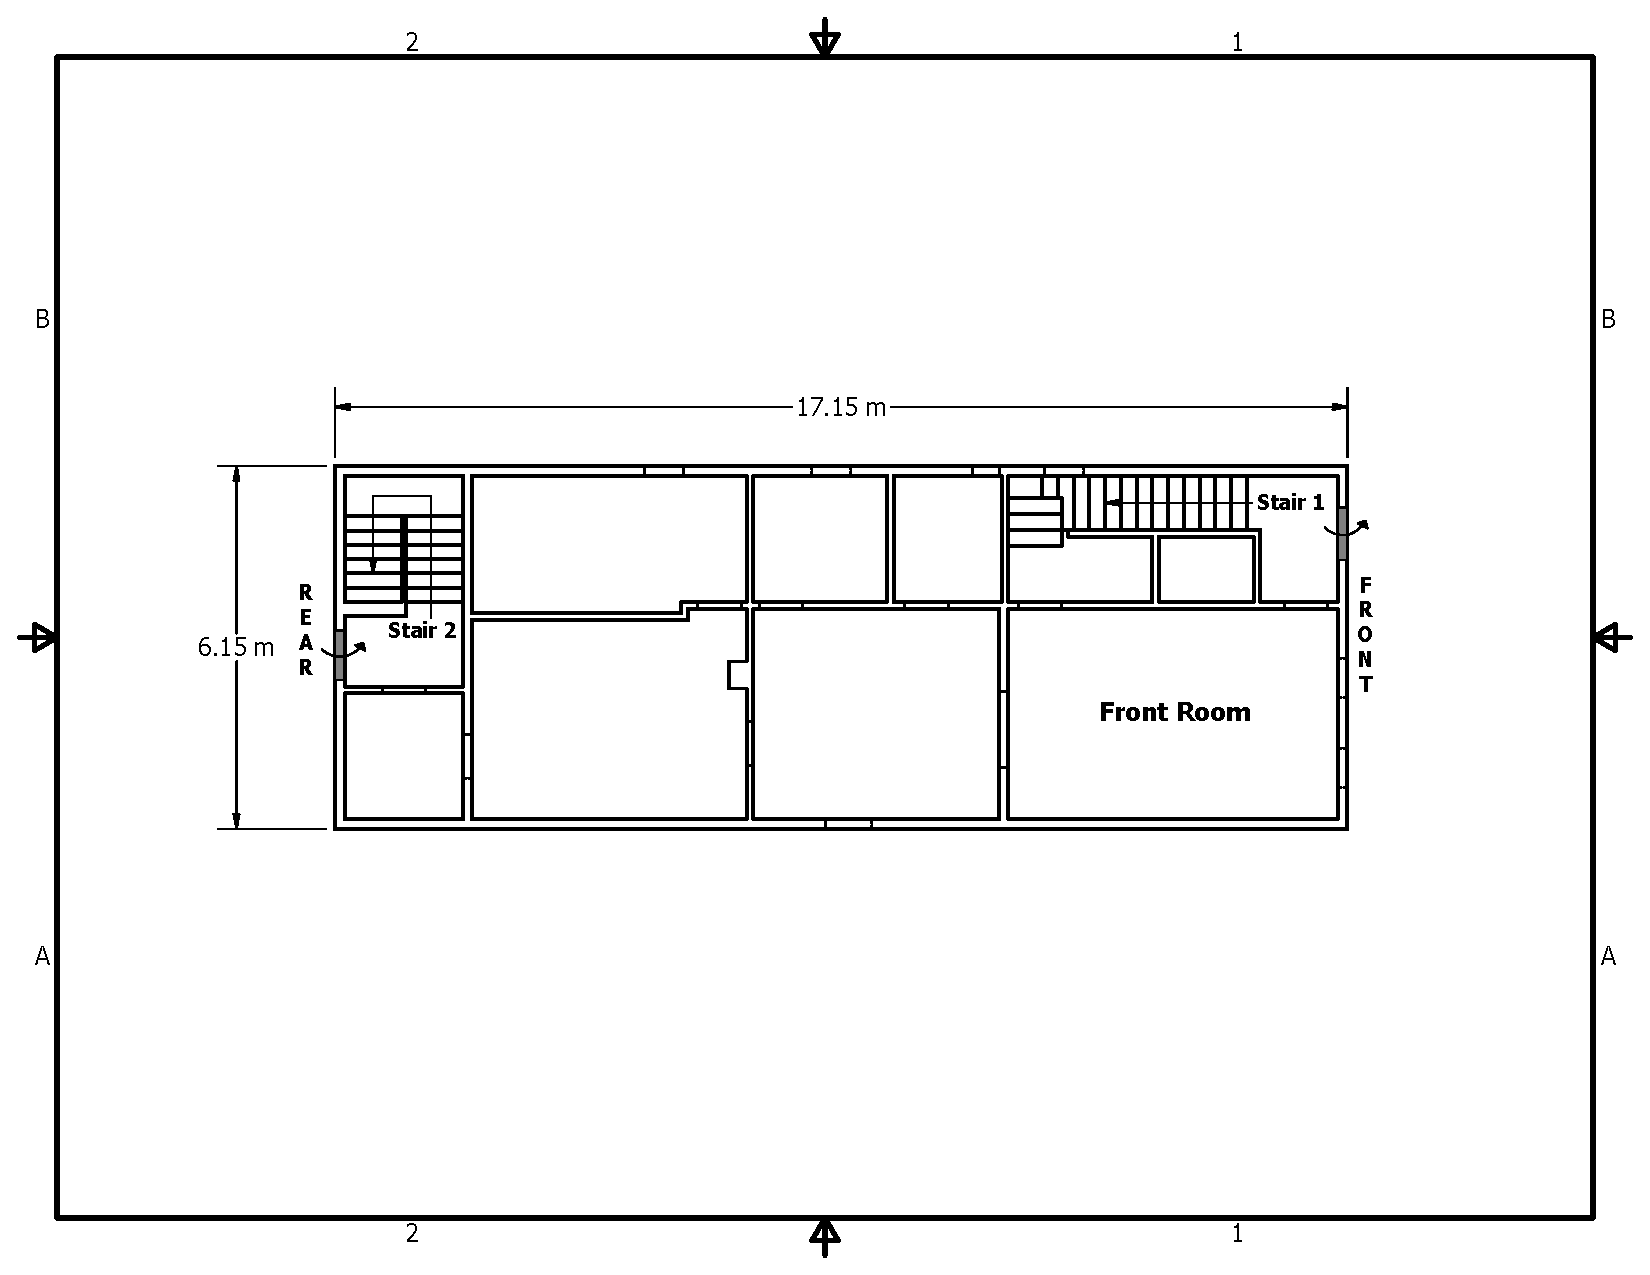
\includegraphics[width=\textwidth]{../Figures/1st_Floor_Metric} \\
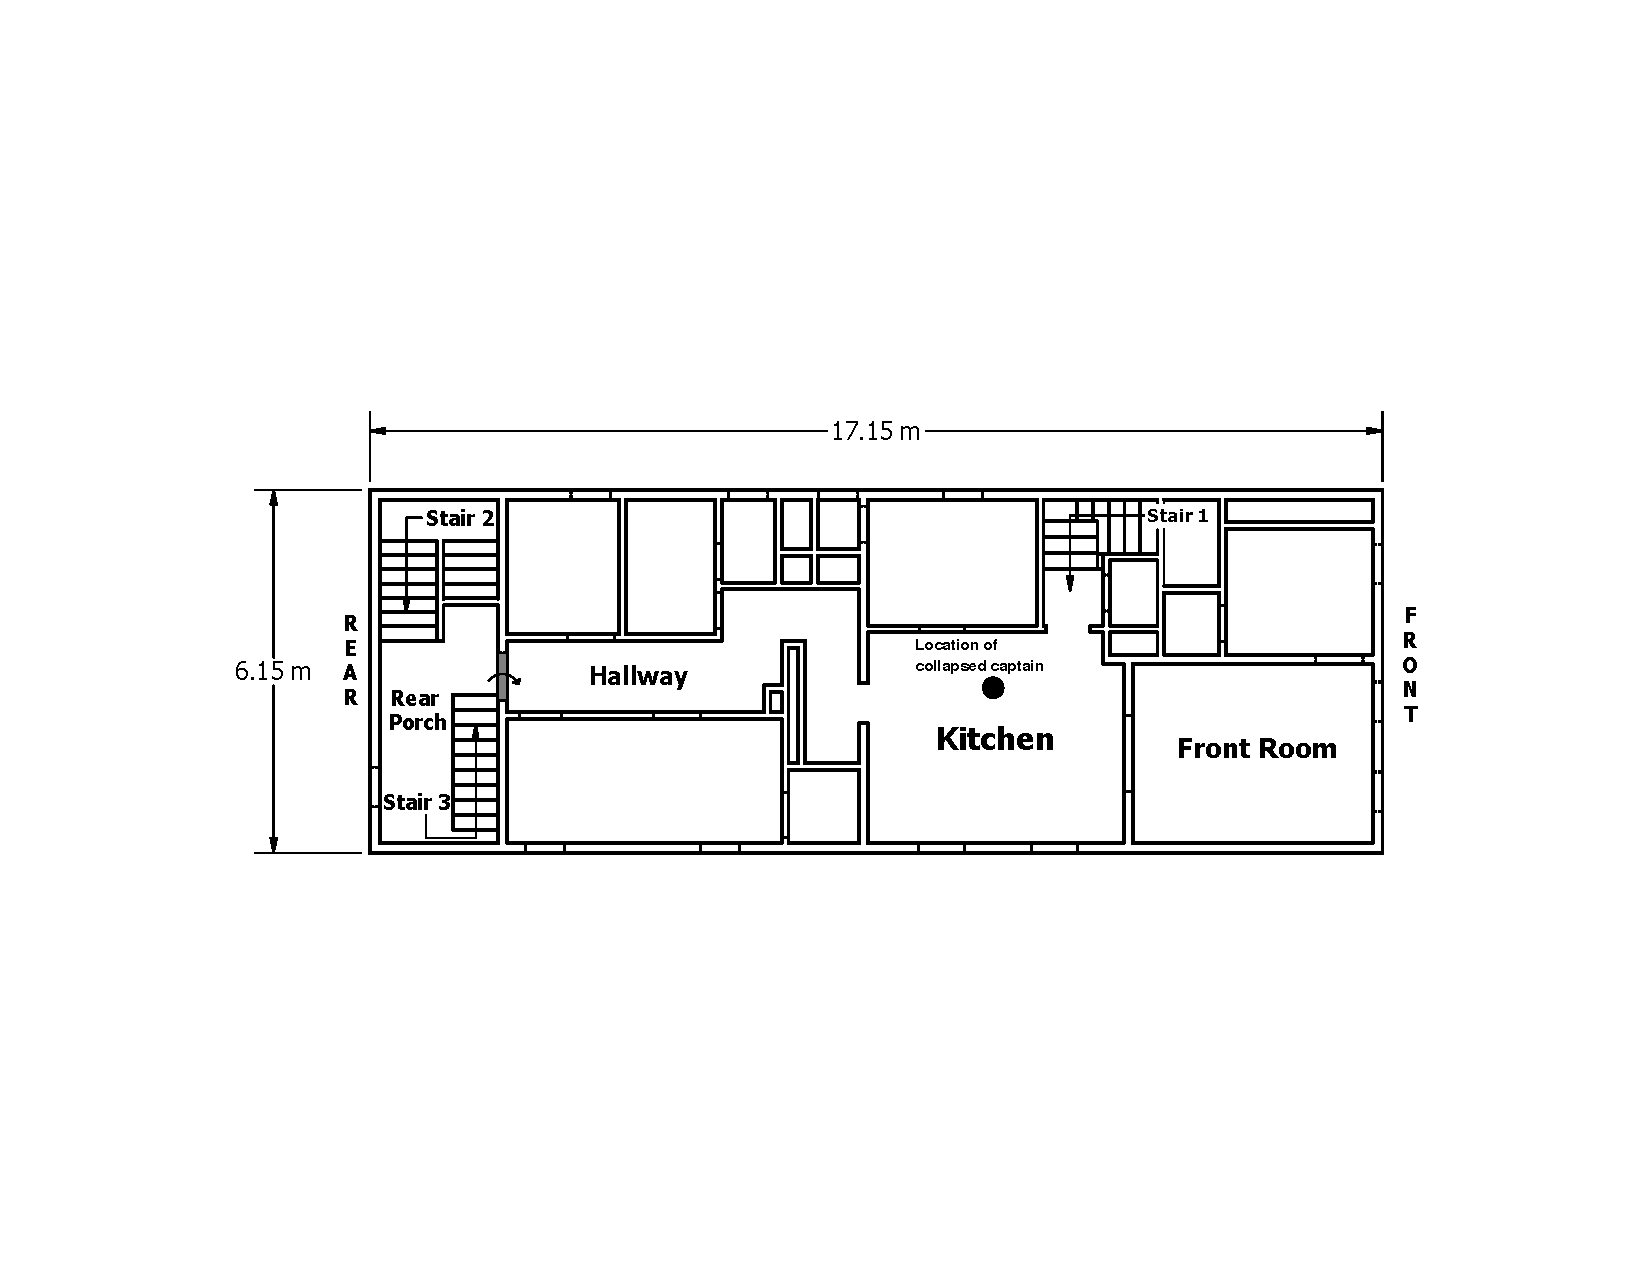
\includegraphics[width=\textwidth]{../Figures/2nd_Floor_Metric}
\end{tabular*}
\caption[Plan view of first (top) and second (bottom) floor of structure.]{Plan view of first (top) and second (bottom) floor of structure. Stairs and key rooms are identified using measurements collected by NIST.}
\label{fig:simp_geom}
\end{figure}

\begin{figure}[!ht]
\centering
\begin{tabular*}{\textwidth}{l@{\extracolsep{\fill}}r}
   \scalebox{1.0}{ 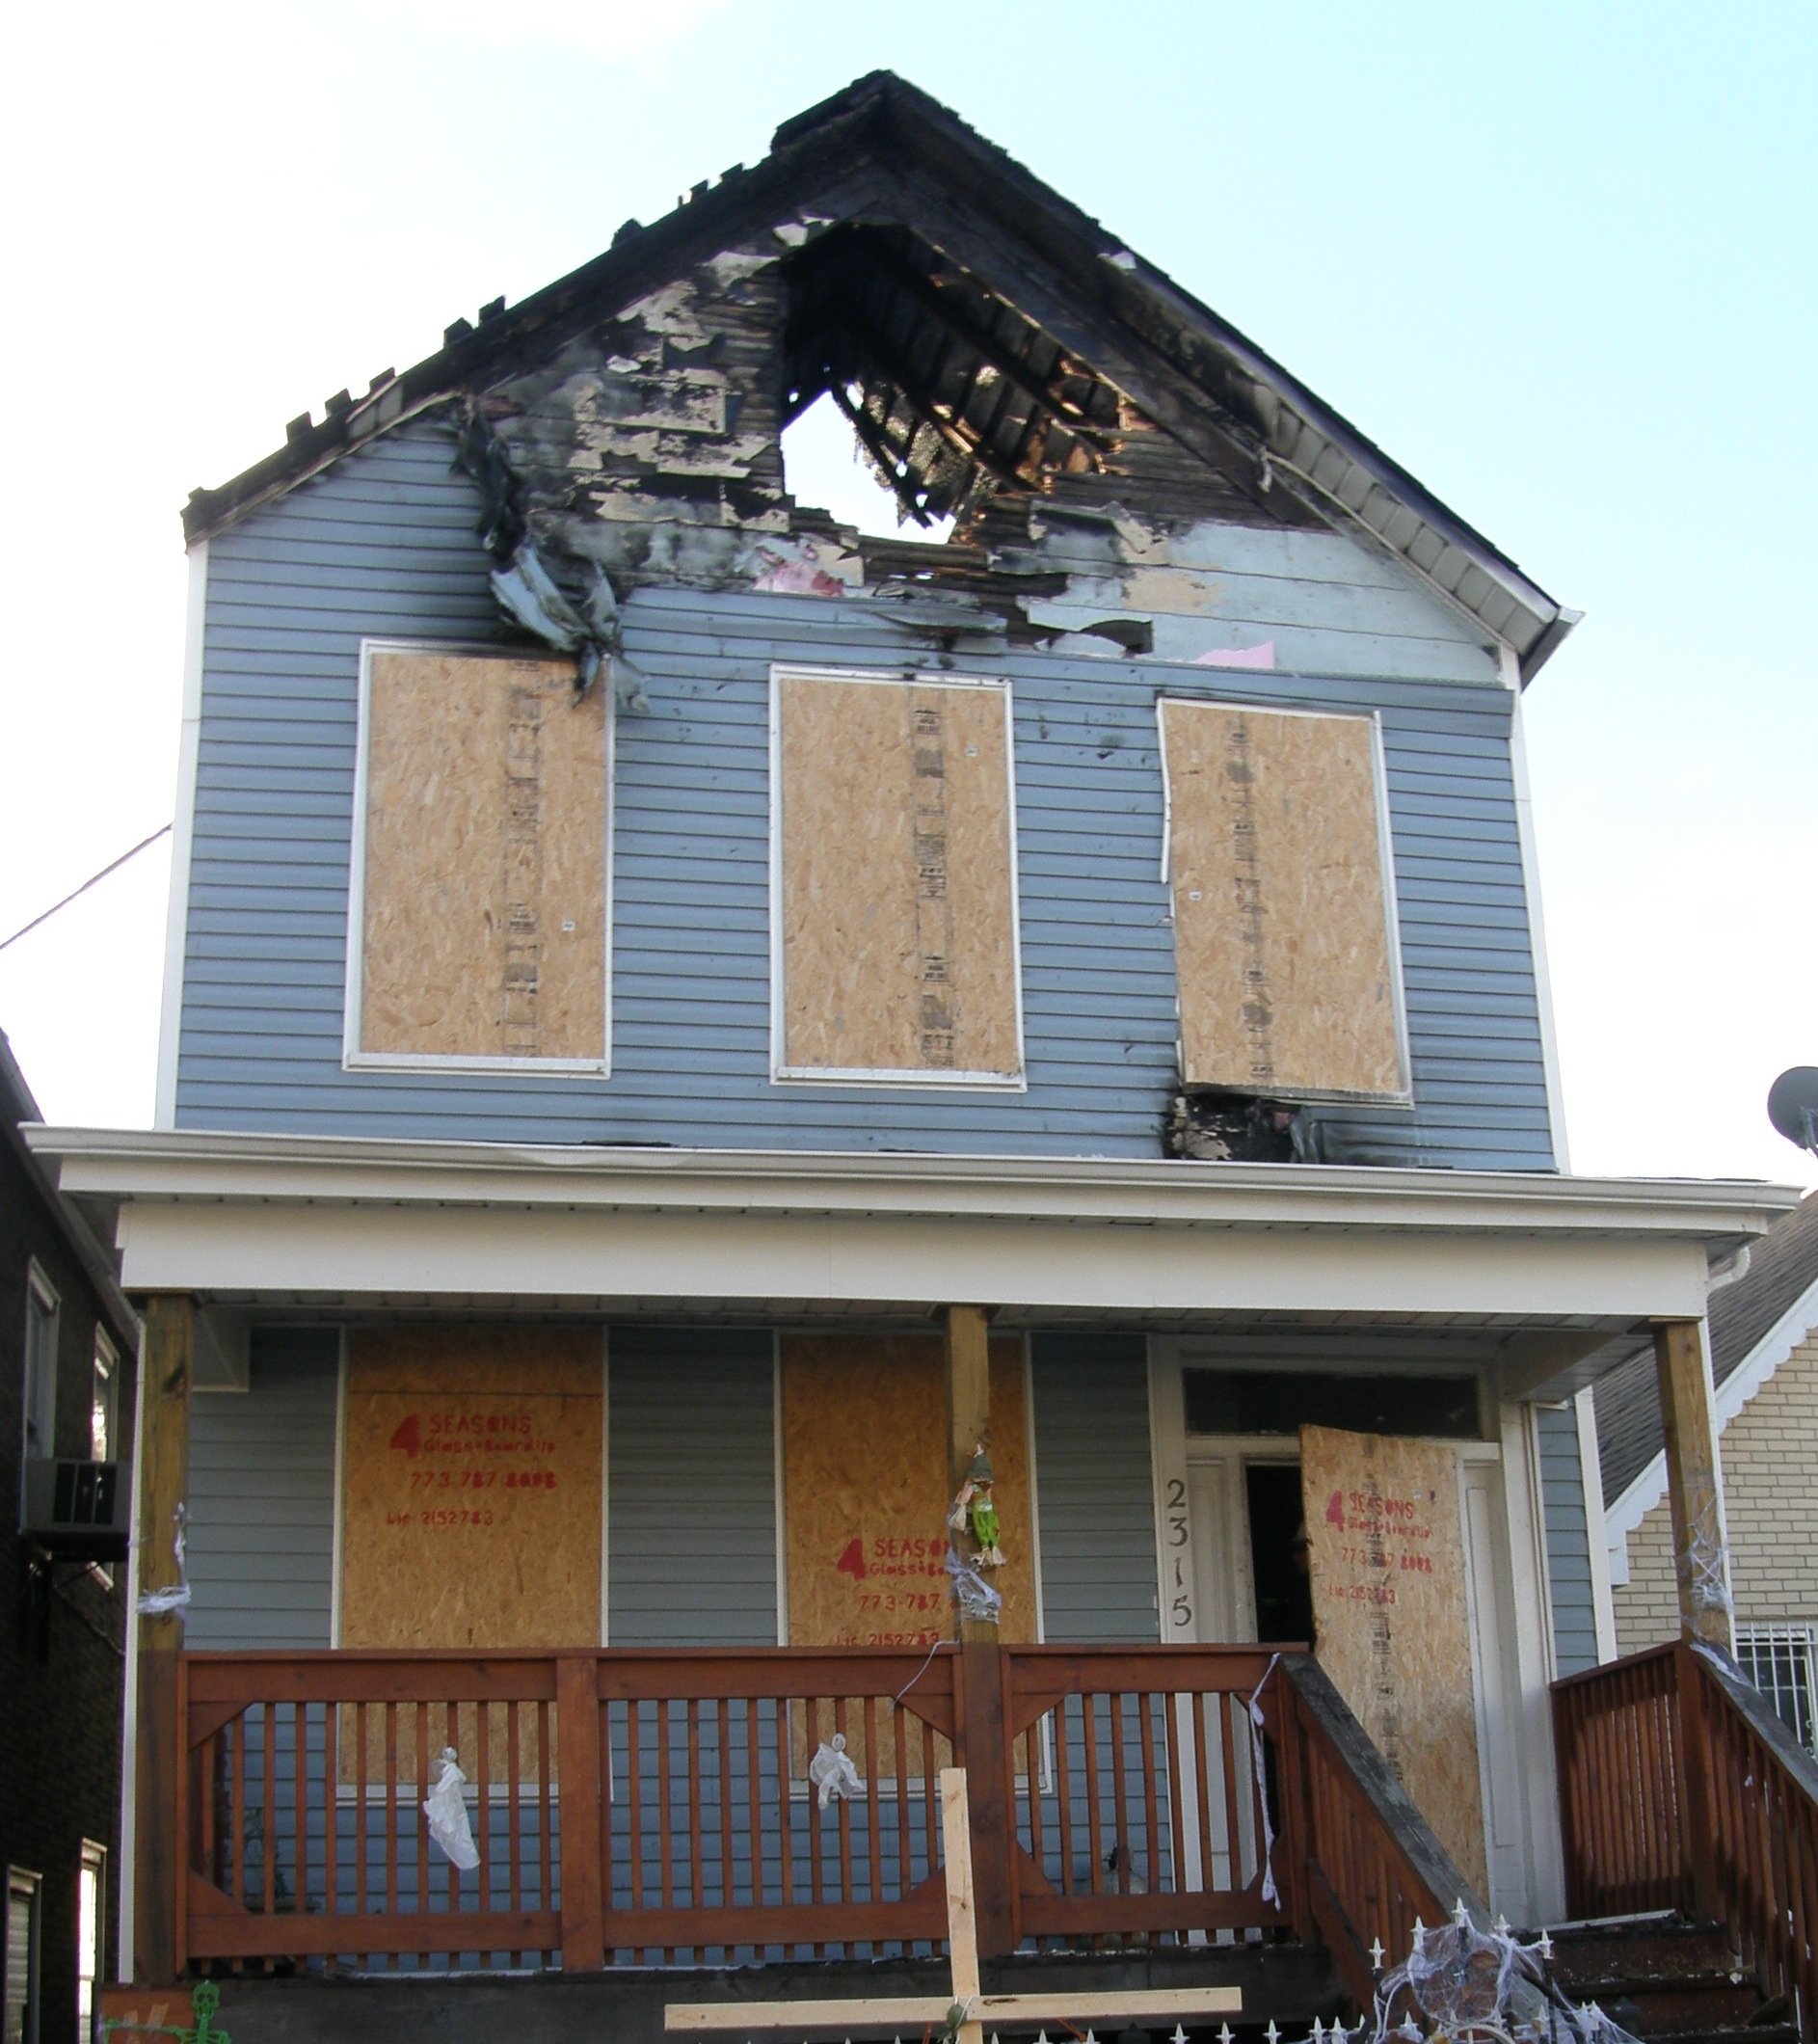
\includegraphics[width=3in]{../Figures/exterior_alpha} } &
   \scalebox{1.0}{ 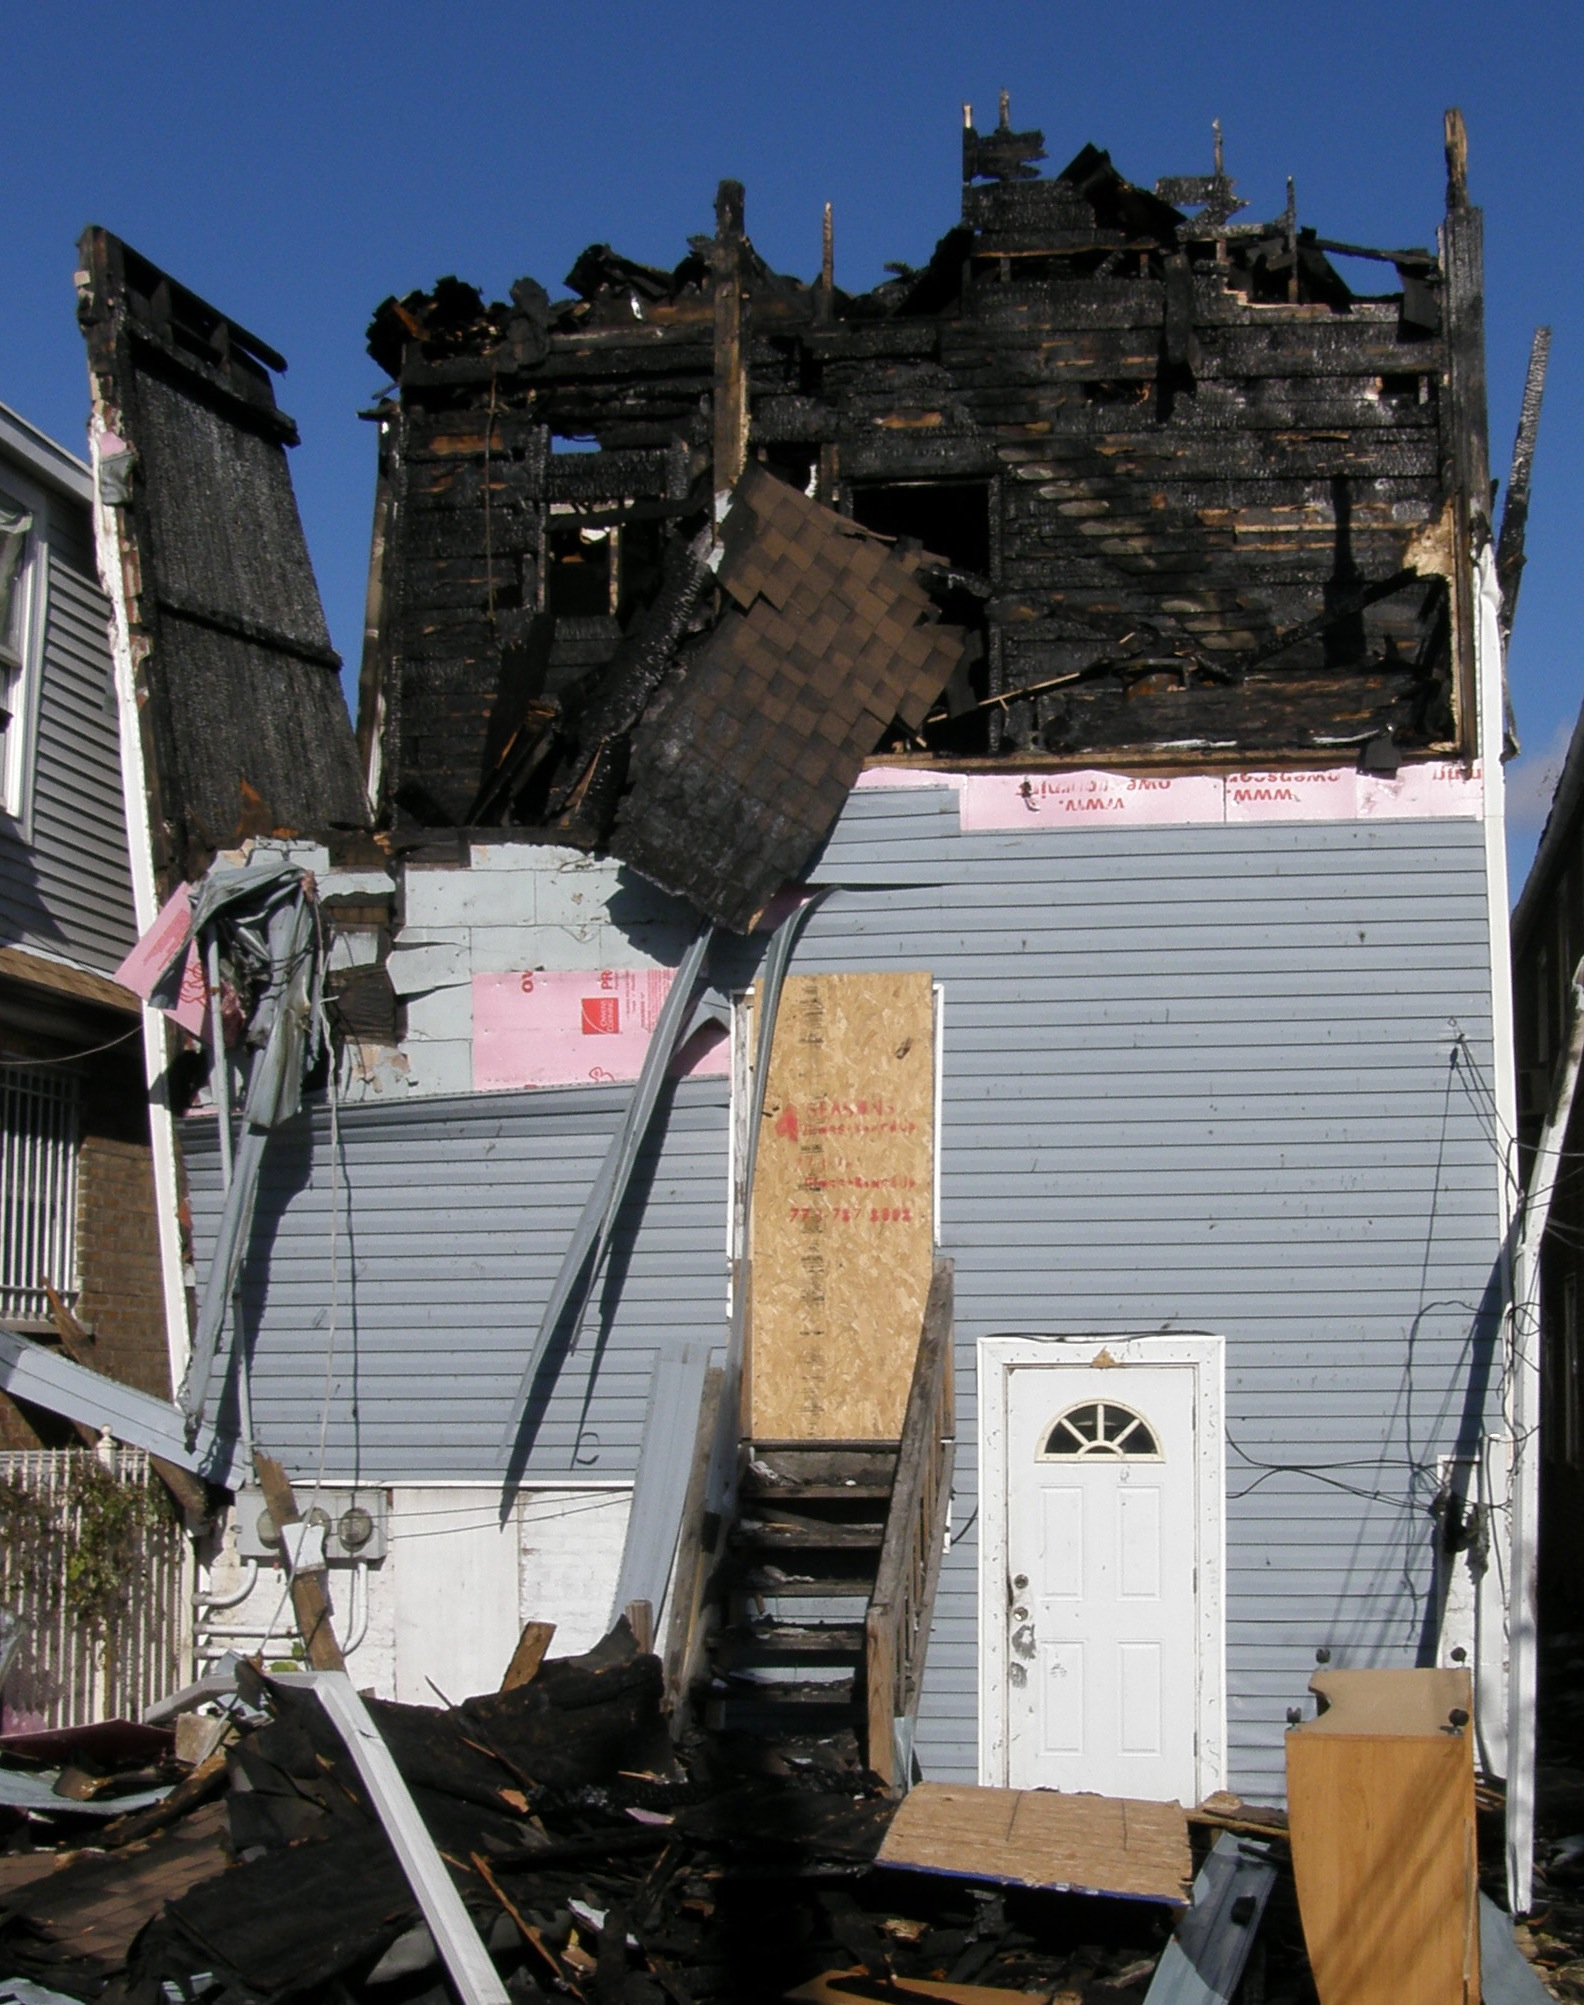
\includegraphics[width=2.67in]{../Figures/exterior_charlie} } \\
\end{tabular*}
\caption{Photographs showing the front (left) and rear (right) exterior of the structure after the incident.}
\label{fig:alpha_ex}
\end{figure}


\clearpage


\section{Fire}
\label{fire}

To estimate the type of fuel, fire size, and structure ventilation, on-scene videos and post-incident reports were used. Based on these sources of information, the FDS model includes two source fire locations: an initial fire in the attic and a secondary fire on the second floor porch landing. The attic and rear porch primarily consisted of wood fuel: the rear porch was enclosed with wood planks covered with foam board and vinyl siding, the roof consisted of asphalt shingles over wood planking, and the attic and porch floors were composed of oriented strand board.

Wood fuel can be represented by the chemical formula, $\C\H_{1.7}\O_{0.74}\N_{0.002}$, with specified yields of carbon monoxide ($y_{\mathrm{CO}}=0.004 \; \mathrm{kg}/\mathrm{kg}$) and soot ($y_{\mathrm{C}}=0.015 \; \mathrm{kg}/\mathrm{kg}$)~\cite{SFPE:Tewarson}. The product yields are expressed in terms of the amount of carbon monoxide or soot emitted per unit mass of fuel consumed (kg/kg) and can be found in the Society of Fire Protection Engineers (SFPE) Handbook~\cite{SFPE:Tewarson}. A balanced chemical reaction for wood combustion can written as:

\begin{multline}
\C\H_{1.7}\O_{0.74}\N_{0.002} + 4.89(0.208\,\O_{2} + 0.783\,\N_{2} + 0.387\text{\sc{e}-}3\,\C\O_{2} + 0.834\text{\sc{e}-}2\,\H_{2}\O) \\ 
\rightarrow 5.84(0.719\text{\sc{e}-}3\,\C\O + 0.168\,\C\O_{2} + 0.155\,\H_{2}\O + 0.669\,\N_{2} + 0.693\text{\sc{e}-}2\,\C)
\label{eq:wood_comb}
\end{multline}

The value for the heat of combustion of wood used in this simulation was~16,400 kJ/kg, based on data provided in the SFPE Handbook~\cite{SFPE:Tewarson}. The heat of combustion quantifies the amount of energy per unit mass of the fuel. The following text defines Eq.~\ref{eq:wood_comb} for an FDS input file with the desired fuel and reaction properties discussed above:

\begin{lstlisting}
&SPEC ID='WOOD', FORMULA='CH1.7O0.74N0.002' /

&REAC ID = 'wood' 
    FUEL = 'WOOD', 
    HEAT_OF_COMBUSTION = 16400,
    SOOT_YIELD = 0.015,
    CO_YIELD = 0.004/
\end{lstlisting}

Note that using the input lines above will invoke the simple chemistry reaction mechanism in FDS in which fuel and air react to form only CO$_2$, CO, H$_2$O, soot, and N$_2$. If the inclusion for other combustion products is desired, then the user must explicitly define those species and the chemical reaction that produces them~\cite{FDS_Users_Guide}. Based on the above input lines, FDS uses the default, mixing-controlled fast chemistry combustion model. This mechanism states that the rate of fuel consumption is proportional to both the local limiting reactant concentration and the local rate of mixing and extinction is based on the critical flame temperature approach~\cite{FDS_Math_Guide}. While FDS provides users with the option to use a more complex finite-rate combustion mechanism, there is not sufficient evidence in this case to justify deviating from the default specifications. 

To estimate the heat release rate per unit area (HRRPUA) of wood, Babrauskas and Grayson~\cite{babrauskas1990} conducted experiments in a cone calorimeter\footnote{The cone calorimeter is an experimental apparatus used to gather data about ignition time, mass loss, combustion products, and heat release rate among other properties associated with burning small samples of materials~\cite{ASTM:E1355}.} to determine the 5-min average of the HRRPUA for several different types of wood over a range of radiant heat fluxes. The results of that study indicate that the HRRPUA for different types of wood is approximately 50~kW/m$^2$.

To calculate the total fire size, the appropriate burning area (exposed wood area) of the attic and second floor porch enclosure needs to be determined. Based on the floor plan of the structure, the underside of the roof was approximately 134~m$^2$ (1453~ft$^2$) with 7~m$^2$ (75~ft$^2$) walls on the front and rear sides. Additionally, there was 105~m$^2$ (1130~ft$^2$) of floor area in the attic. Examination of post-incident images indicated that the floor immediately over the rear porch burned away. That area was considered to be part of the porch fire. Based on post-incident damage, approximately 50~\% of the remaining floor area and 90~\% of the roof was considered to be fuel for the attic fire. To estimate the total attic fire size, the underside roof area (120~m$^2$), two end walls (14~m$^2$), and the floor area (43~m$^2$ or 463~ft$^2$) were included. Applying an HRRPUA of wood of 50~kW/m$^2$ results in a potential peak fire size of 9~MW. To estimate the size of the porch fire, the four walls of the porch enclosure (42~m$^2$ or 452~ft$^2$) and the floor and ceiling of the porch (24~m$^2$ or 258 ft$^2$) were included, which results in a total porch area of 66~m$^2$ (689~ft$^2$). Using the same HRRPUA of wood of 50~kW/m$^2$, the potential peak fire size on the porch was approximately 3.3~MW. Therefore, the maximum fire size for this structure was estimated to be 12.3~MW. Since the time at which the fire started is not known relative to the notification of a fire or how fast the fire spread, several simplifications were made. The first assumption is that the attic fire was specified to start at the beginning of the simulation and increase to a value of 9~MW in 10~s. The porch fire was specified to start 40~s into the simulation and increase to a value of 3.3~MW in 10~s. The 10-s ramp up time was used to prevent abrupt changes in the velocity at the fire boundary condition in FDS. The second assumption is that the sources of the gas phase wood fuel have constant areas at fixed locations (2 sources for the attic, 1 source for the porch). The following lines define the source fires in the FDS input file:

\begin{lstlisting}
&SURF ID='FIRE', HRRPUA=2250., COLOR='ORANGE', TAU_Q=10 /
&VENT XB=-13.5,-13,1,5,6.16,6.16, SURF_ID='FIRE' / 
&VENT XB=-14.5,-14,1,5,6.16,6.16, SURF_ID='FIRE' / 
&VENT XB=-16.5,-15.5,1,2.5,3.14,3.14, SURF_ID='FIRE', DEVC_ID='SECOND FIRE'/ 
&DEVC XYZ = -17.2,2,0, ID='SECOND FIRE', QUANTITY='TIME', SETPOINT=40, INITIAL_STATE=.FALSE. /
\end{lstlisting}
Note that the coordinates here are unique for the vents are specific to the input files used for these simulations. The key point is that they are 2-D planes located at a specific area.


\clearpage


\section{Materials}
\label{matl}
While the fires were represented as fuel sources with a constant area (Section~\ref{fire}), from a heat transfer perspective, it is important to define the material properties (density, thermal conductivity, and specific heat) to account for heat transfer and energy storage in the ceiling, walls, and floor. In this study, the material properties of gypsum board~\cite{WAKILI2007} were specified on the finished walls and ceilings on the main two floors of the structure, and the material properties of wood~\cite{Incropera:1} were specified on the unfinished portions of the attic and rear porch. The following lines define these materials in the FDS input file:

\begin{lstlisting}
&MATL ID = 'GYPSUM BOARD'
    FYI = 'Wakili - Journal of Fire Sciences 2007' 
    CONDUCTIVITY = 0.28
    SPECIFIC_HEAT = 1.0
    DENSITY = 810. /

&MATL ID = 'WOOD MAT'
    FYI = 'Incropera and DeWitt, Fundamentals of Heat and Mass Transfer'
    CONDUCTIVITY = 0.12
    SPECIFIC_HEAT = 1.38
    DENSITY = 510. / 
\end{lstlisting}

\section{Ventilation}
\label{Vents}
The simulations in this study account for changes in the ventilation due to a combination of fire department operations (opening doors) and fire acting on the structure (fire breaching walls, breaking windows, etc). Two different ventilation scenarios were considered in this study. The first scenario involves a baseline simulation in which the ventilation times and ventilation areas represent our best understanding of the incident. The second scenario, or alternative simulation, does not include the firefighter opening the rear door to make entry to the structure and the subsequent exterior left wall fire penetration. The times of the ventilation changes are provided in Table~\ref{tab:vents}. Structure leakage has been shown to be important when modeling enclosure fires~\cite{beal2009}. The open front door at the start of the simulation and the vents (opening size and open time) created during the simulation are significantly larger than the total effective area of leakage of a structure of this type. Therefore, any leakage in the structure would have a negligible impact on the fluid mechanics within the structure and is not included in this study.

An unknown parameter in Table~\ref{tab:vents} that needed to be estimated was the time when the second floor interior/porch door failed (160~s into the simulation). The area of failure was also estimated based on the following observations. The bottom hinge from the door appeared to be closed throughout the fire due to the lack of fire damage and the lack of soot deposited on the interior faces of the hinge and remaining wood, as shown in Fig.~\ref{fig:door_frame}. It appears that the door collapsed and failed partially open. In the simulations, only the upper portion of the door was assumed to fail. While this time and area may not be exact, the takeaway from the analysis in the following sections should be impact of the door's failure on the interior conditions of the structure.

\clearpage

\begin{table}
\centering
\captionof{table}{Timeline of ventilation changes in the simulation}\label{tab:vents}
\begin{tabular}{cccll}
\toprule[1.5pt]
Baseline    &  Alternative  &  Ventilation  &  Type         &  Side of         \\
Simulation  &  Simulation   &  Area         &               &  Structure       \\
{[s]}       &  {[s]}        &  [m$^2$]      &               &                  \\
\midrule
0           &  0            &  0.11         &  Window       &  Rear            \\
40          &  40           &  0.08         &  Breach (x2)  &  Front and Rear  \\
45          &  45           &  0.12         &  Breach       &  Left            \\
55          &  55           &  0.12         &  Breach       &  Rear            \\
130         &  N/A$^*$      &  1.41         &  Door         &  Rear            \\
135         &  N/A$^*$      &  0.2          &  Breach       &  Left            \\
160         &  160          &  0.80         &  Door         &  Interior        \\
\bottomrule[1.25pt]
\end{tabular}\par
\footnotesize
$^*$These ventilation events were not included in the alternative simulation.
\normalsize
\end{table}

\begin{figure}[!ht]
\centering
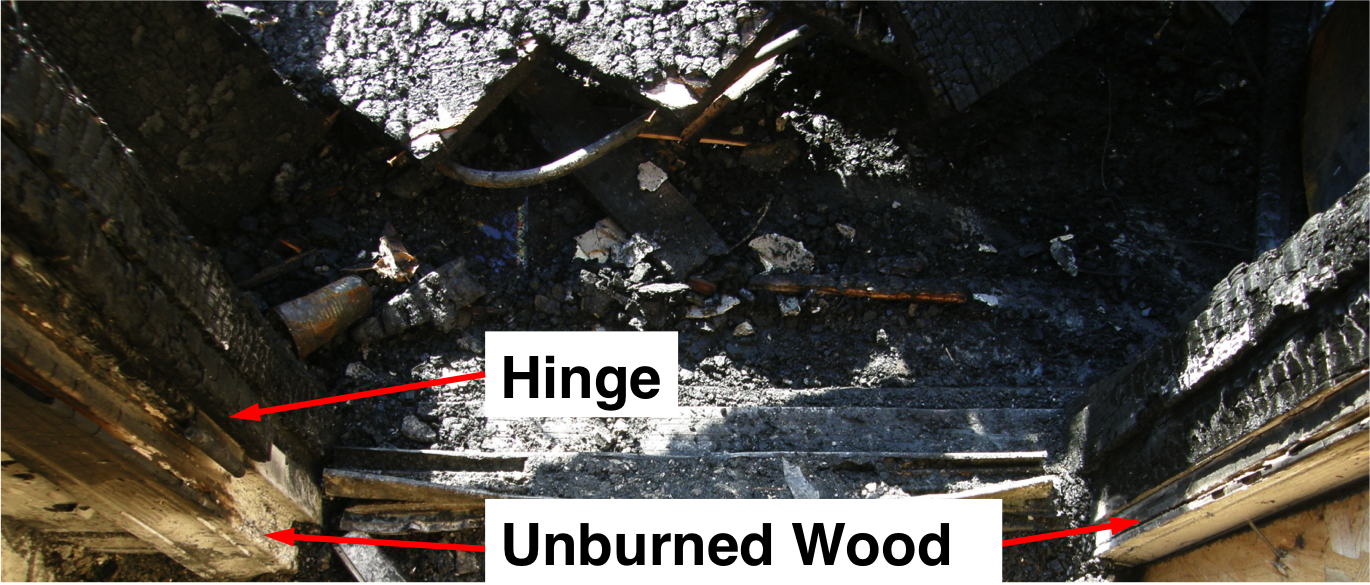
\includegraphics[width=.80\textwidth]{../Figures/door_frame_burn}
\caption[Post-incident image of rear porch door frame.]{Post-incident image of the second floor porch door frame that failed taken from inside the structure looking toward the porch. Note that the hinge is still intact and there is unburned, ``clean'' wood along the bottom portion of the frame.}
\label{fig:door_frame}
\end{figure}


\clearpage


\section{Numerical Mesh}
\label{mesh}

For the simulation, a measure of how well the flow field is resolved can be estimated by using the non-dimensional expression $D^*/\dx$. Here, $D^*$ is the characteristic fire diameter, $\dx$ is the nominal size of a mesh cell, and $\dQ$ is the total heat release rate of the fire:
\begin{equation}
D^* = \left(
     \frac{\dQ}{\rho_\infty \, c_p \, T_\infty \, \sqrt{g}}
     \right)^\frac{2}{5} 
\label{eq:mesh}
\end{equation}   
From the FDS User's Guide~\cite{FDS_Users_Guide}, the characteristic fire diameter is related to the characteristic fire size via the
relation $Q^* = (D^*/D)^{5/2}$. Here, $D$ is the physical diameter of the base of the fire specified in the simulation. Following Eq.~\ref{eq:mesh} and using a grid cell size of 10~cm, the characteristic fire diameter to cell size ($D^*/\dx$) ratio is 15.5 for the 3.3~MW porch fire and 23 for the 9~MW attic fire. Based on validation work performed for the U.S. Nuclear Regulatory Commission, $D^*/\dx$ values ranged between 4 and 16~\cite{NUREG_1824} and produced results that were adequate for engineering calculations. The grid resolution used in this model is within or exceeds typical engineering $D^*/\dx$ values.

As discussed in Section~\ref{geom}, the structure has dimensions of 17.15~m (56~ft) by 6.15~m (20~ft) and a total height of 8.56~m (28~ft). To ensure adequately resolved fluid flow in and out of the structure, the computational domain was extended beyond the volume of the structure. The total volume of the computational domain was 24~m (79~ft) by 10~m (33~ft) by 10~m (33~ft). A grid resolution of 10~cm (3.9~in) was used, which required 2.4 million computational cells. As a result, all of the input model geometry lengths, ventilation openings (holes, doors, and windows), and fire areas will snap to the nearest 10~cm. Figure~\ref{fig:geom_grid} shows the front of the structure rendered in Smokeview with the 10~cm mesh. The domain was divided into 16 equally sized meshes (each containing 150,000 grid cells) that could be processed in parallel, which reduced the amount of required calculation time to approximately 1.5~days. Figure~\ref{fig:mult_mesh} shows the entire structure within the computational domain that has been divided into multiple meshes. Table~\ref{tab:mod_param} shows a summary of the model input parameters for the simulations that were conducted as part of this study.

\begin{figure}[!ht]
\centering
\begin{tabular*}{\textwidth}{l@{\extracolsep{\fill}}r}
   \scalebox{1.0}{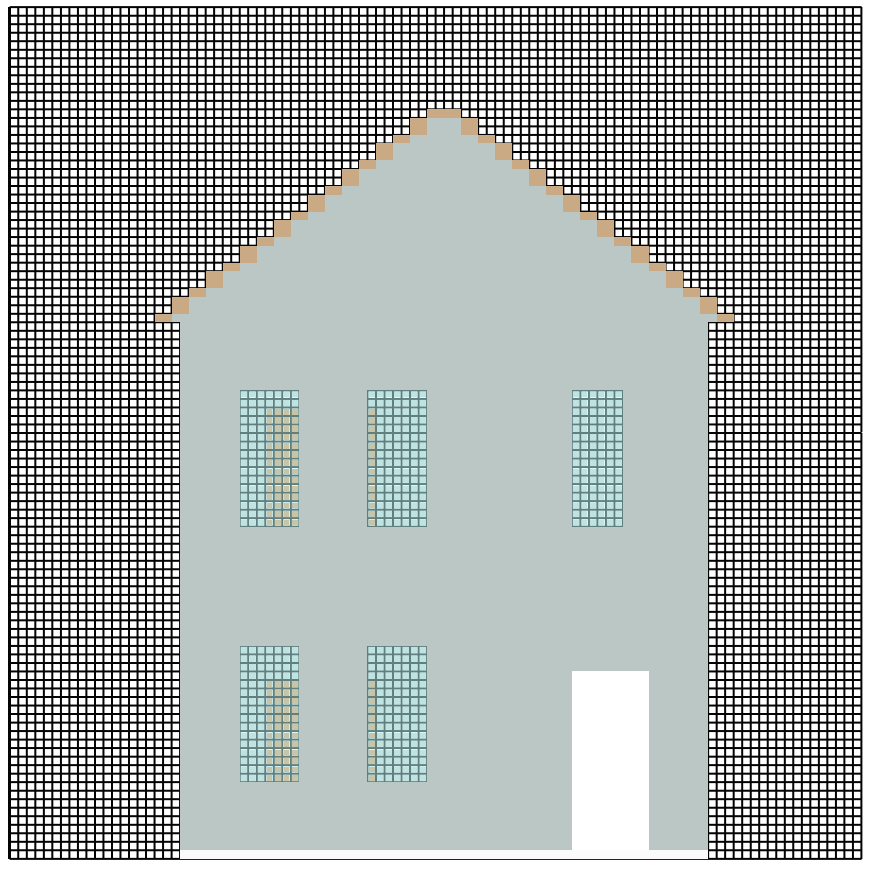
\includegraphics[width=.49\textwidth]{../Figures/smv_exterior_grid}} &
   \scalebox{1.0}{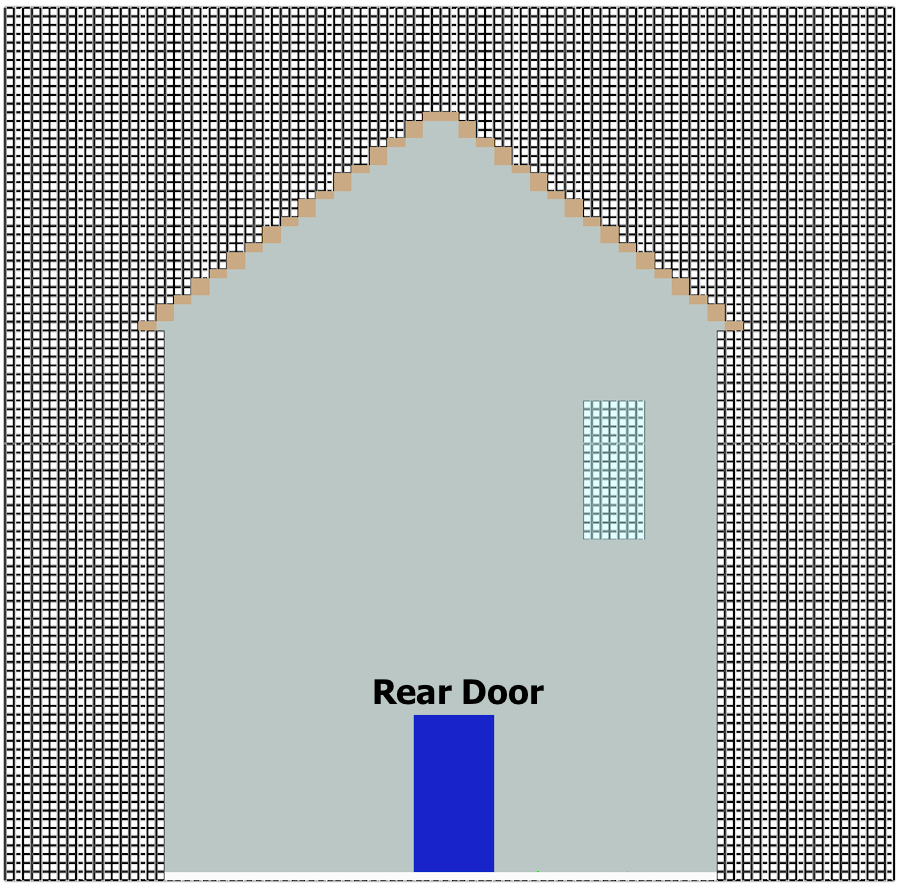
\includegraphics[width=.488\textwidth]{../Figures/smv_exterior_grid_rear}} \\
\end{tabular*}
\caption{Front (left) and rear (right) of the structure with 10~cm computational mesh.}
\label{fig:geom_grid}
\end{figure}

\begin{figure}[!ht]
\centering
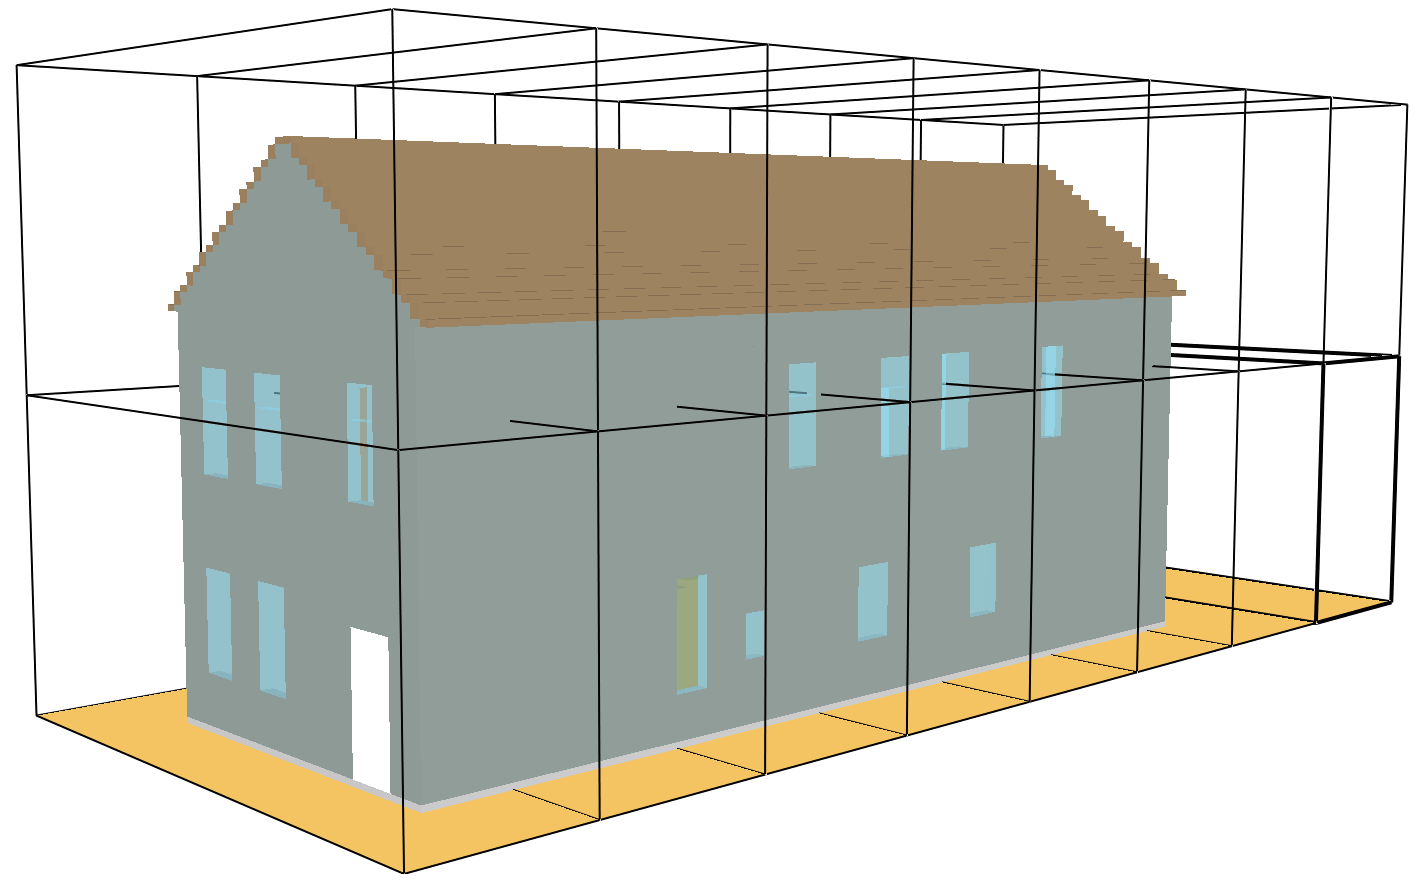
\includegraphics[width=.60\textwidth]{../Figures/smv_exterior_mesh}
\caption[Front-right side of the structure within the computational domain.]{Front-right side of the structure within the computational domain (with multiple meshes). Each of the 16 meshes is 3~m (9.8~ft) by 10~m (33~ft) by 5~m (16.4~ft).}
\label{fig:mult_mesh}
\end{figure}

\begin{table}
\centering
\captionof{table}{Relevant fire model input parameters}\label{tab:mod_param}
\begin{tabular}{lll}
\toprule[1.5pt]
Parameter                                                  & Description                                   & Discussion                            \\
\midrule
Simulation Time                                            &  5~min                                        & --                                    \\ [.25cm]
Grid Cell Size                                             &  10~cm                                        & Section~\ref{mesh}                    \\ [.25cm]
Ambient Temperature$^*$                                    &  20~$^{\circ}$C (77~$^{\circ}$F)              & --                                    \\ [.1cm]
\multirow{4}{*}{Reaction: Wood~\cite{SFPE:Tewarson}}       &  Formula: $\C\H_{1.7}\O_{0.74}\N_{0.002}$     & \multirow{4}{*}{Section~\ref{fire}}   \\
                                                           &  CO Yield: 0.004~$\mathrm{kg}/\mathrm{kg}$    &                                       \\
                                                           &  Soot Yield: 0.015~$\mathrm{kg}/\mathrm{kg}$  &                                       \\
                                                           &  Heat of Combustion: 16,400~kJ/kg             &                                       \\ [.25cm]
\multirow{2}{*}{Peak HRR}                                  &  Attic Fire: 9~MW                             & \multirow{2}{*}{Section~\ref{fire}}   \\ 
                                                           &  Porch Fire: 3.3~MW                           &                                       \\ [.25cm]                     
\multirow{3}{*}{Material: Wood~\cite{Incropera:1} }        &  $k$: 0.12~\si{W/(m.K)})                      & \multirow{3}{*}{Section~\ref{matl}}   \\
                                                           &  $\rho$: 510~kg/m$^3$                         &                                       \\
                                                           &  $c_{p}$: 1.38~\si{kJ/(kg.K)}                 &                                       \\ [.25cm]
\multirow{3}{*}{Material: Gypsum Board~\cite{WAKILI2007}}  &  $k$: 0.28~\si{W/(m.K)}                       &  \multirow{3}{*}{Section~\ref{matl}}  \\ 
                                                           &  $\rho$: 810~kg/m$^3$                         &                                       \\ 
                                                           &  $c_{p}$: 1.0~\si{kJ/(kg.K)}                  &                                       \\
\bottomrule[1.25pt]
\end{tabular}\par
\footnotesize
$^{*}$ Initial interior temperatures were assumed to be 20~$^{\circ}$C; exterior temperatures were 7~$^{\circ}$C~\cite{NIOSH:Bowyer}.
\normalsize
\end{table}

\chapter{Model Results}
\label{results}

To examine the results of the simulations, it is important to link the timelines from the fire scene to the simulation times. Table~\ref{tab:firesim} shows the fireground timeline~\cite{NIOSH:Bowyer} along with the corresponding simulation times.

\begin{table}
\centering
\captionof{table}{Fire incident and simulation event timeline}\label{tab:firesim}
\begin{tabular}{ccl}
\toprule[1.5pt]
Incident Time  &  Simulation Time  &  Fire Behavior / Fireground Operation  \\
{[hh:mm:ss]}   &  {[s]}            &                                        \\
\midrule
\multirow{2}{*}{17:15:00} &    & \multirow{2}{*}{\parbox{9cm} {Fire is reported with heavy smoke coming from the front and rear of the structure's attic.}} \\ 
         & & \\[.25cm] %blank rows exist for wrapping text. # of blanks is 1 less than number of rows
\multirow{2}{*}{17:16:00} & \multirow{2}{*}{}   &  \multirow{2}{*}{\parbox{9cm} {Dispatch for a ``Still'' alarm - two engine companies, two truck companies, and a battalion chief.}} \\
         & & \\[.25cm]
\multirow{3}{*} {} &  \multirow{3}{*} {0} &  \multirow{3}{*}{\parbox{8cm} {FDS simulation starts. Attic fire ignites. Initial ventilation through rear of structure. Front door open.}} \\
         & & \\[0.25cm]
         & & \\[0.25cm]
\multirow{3}{*}{17:20:00} & \multirow{3}{*}{40}  & \multirow{3}{*}{\parbox{9cm} {Attic windows break - heavy smoke out of front attic window and heavy smoke and fire out of rear. Rear porch ignites in model.}} \\
         & & \\[.25cm]
         & & \\[.25cm]  
\multirow{2}{*}{}  & \multirow{2}{*}{45} & \multirow{2}{*}{\parbox{8cm}{Ventilation through wall penetration on rear of structure.}} \\
          & & \\[.25cm] 
\multirow{2}{*}{}  & \multirow{2}{*}{55}  & \multirow{2}{*}{\parbox{8cm}{Ventilation through wall penetration on left side of structure.}} \\ 
          & & \\[.25cm] 
\multirow{2}{*}{17:21:00} & \multirow{2}{*}{100} & \multirow{2}{*}{\parbox{8cm}{E123 captain and firefighter on second floor with 1\sfrac{3}{4}-inch hoseline.}} \\
         &  & \\[.25cm]
\multirow{2}{*}{17:21:30} & \multirow{2}{*}{130} &  \multirow{2}{*}{\parbox{8cm}{First floor exterior porch door opened. Porch fire ignites in FDS model.}} \\
        &  & \\[.25cm]
        & 135 & Ventilation through left side of structure. \\[.25cm] 
        & 160 & Top of interior door fails in FDS model. \\[.25cm] 
\multirow{3}{*}{17:23:00}    & \multirow{3}{*}{220} & \multirow{3}{*}{\parbox{8cm} {Heavy fire report in rear stairwell and enclosed porch. No response from E123 captain or firefighter.}} \\
         & & \\[.25cm]
         & & \\[.25cm]  
17:24:00    &   & Water applied to attic from the rear exterior position. \\[.25cm]
17:25:00    &   & SQ5 makes entry through front of structure. \\[.25cm]
\multirow{2}{*}{17:27:00}    & \multirow{2}{*}{300}  & \multirow{2}{*}{\parbox{8cm} {After hearing a Mayday call from SQ5, IC calls a Mayday. Simulation ends.}}\\
         & &  \\[.25cm]
17:29:00    &   & E123 captain carried out of structure. \\
\bottomrule[1.25pt]
\end{tabular}\par
\footnotesize
For specific information regarding ventilation areas used in the FDS model, refer to Table~\ref{tab:vents}.
\normalsize
\end{table}


\section{Heat Release Rate}
\label{HRR}
The heat release rate output data from FDS quantifies the simulated rate of energy release in the simulation. Figure~\ref{fig:hrr} shows the prescribed HRR versus time values based on the prescribed fires along with the FDS results for the two ventilation scenarios that were described in Section~\ref{Vents}. The two vertical lines represent the time at which a firefighter opened the back door of the structure ($t$ = 130 s) and the time at which the second floor interior door was estimated to fail ($t$ = 160 s). Due to a lack of information about the time of fire ignition or how fast the fire grew, these parameters needed to be estimated.  The growth rate shown in Fig.~\ref{fig:hrr} (10~MW in approximately 20~s) is fast because the incipient stage of the fire growth was not considered in this study. The maximum size of the fire used in this study was selected such that the conditions would become ventilation limited quickly to minimize computational time while aligning with the timeline observations of video and picture evidence from the fire. Using this approach, the accuracy of heat transfer to the walls of the structure may be sacrificed; however, all of the window, door, and wall failures were driven by the event timeline rather than failure temperature criteria.

\begin{figure}[!ht]
\centering
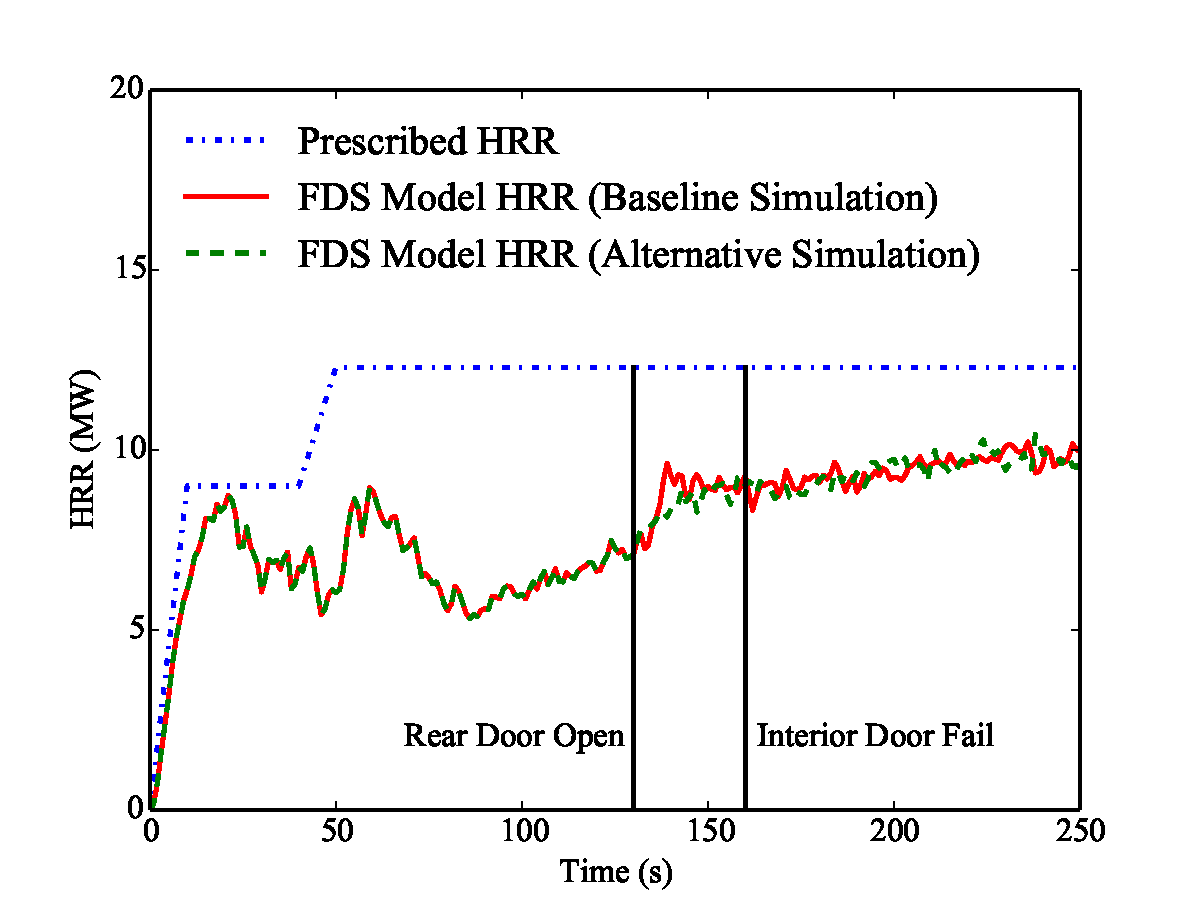
\includegraphics[width=.80\textwidth]{../Figures/Chicago_Fire_HRR}
\caption[HRR versus time from the FDS simulations.]{HRR versus time from the FDS simulations. The first vertical line indicates the time at which the back door failed (130~s), and the second vertical line indicates the time at which the interior hallway door failed (160~s).}
\label{fig:hrr}
\end{figure}

In Fig.~\ref{fig:hrr}, the solid line represents the baseline FDS simulation (this follows the noted door openings from the incident). The dashed line represents an alternative series of events in which the rear door does not get opened and the subsequent breach of the rear porch wall on the left side of the structure does not occur. The dash-dotted line represents the prescribed (or nominal) HRR that was input into FDS. As shown in Fig.~\ref{fig:hrr}, the HRR output from FDS is less than the prescribed HRR because the fire in the structure becomes ventilation limited. The maximum HRR value is slightly less than 9~MW before the fire becomes ventilation limited and begins to decay. The HRR is reduced to 5~MW as the oxygen inside the structure is consumed. There is an insufficient amount of oxygen in the structure to combust all of the fuel, therefore combustion occurs locally at the vents where fresh air is available. Figure~\ref{fig:smv_ext_fire} shows flaming combustion through the failed window on the rear side of the structure and attic breach just after the second fire ignites at 40~s. After additional wall breaches occur at 45~s and 55~s (see Table~\ref{tab:vents}), the abrupt change in ventilation causes the HRR to increase to 9~MW before it decreases to approximately 6~MW. The HRR then increases towards a sustainable steady-state value.

Figure~\ref{fig:hrr} indicates that the HRRs for both of the ventilation scenarios in FDS are identical until 130~s (HRR $\approx$ 7~MW). At 130~s, the rear door is opened in the baseline simulation. At 135~s, there is an additional breach on the left side of the structure (Table~\ref{tab:vents}). The open door and breach act as additional pressure releases for the structure. Again, the abrupt change in ventilation causes the HRR to increase from approximately 7~MW to 9.7~MW at 139~s. At the time of the door failure (160~s), the HRR in both cases was approximately 9~MW because of the increased amount of ventilation. While there might be some locally different burning characteristics between the baseline simulation and the alternative simulation, the interior conditions in both cases presented a significant hazard to firefighters inside of the structure. Therefore, the analysis will focus on the results of the baseline simulation.

\begin{figure}[!ht]
\centering
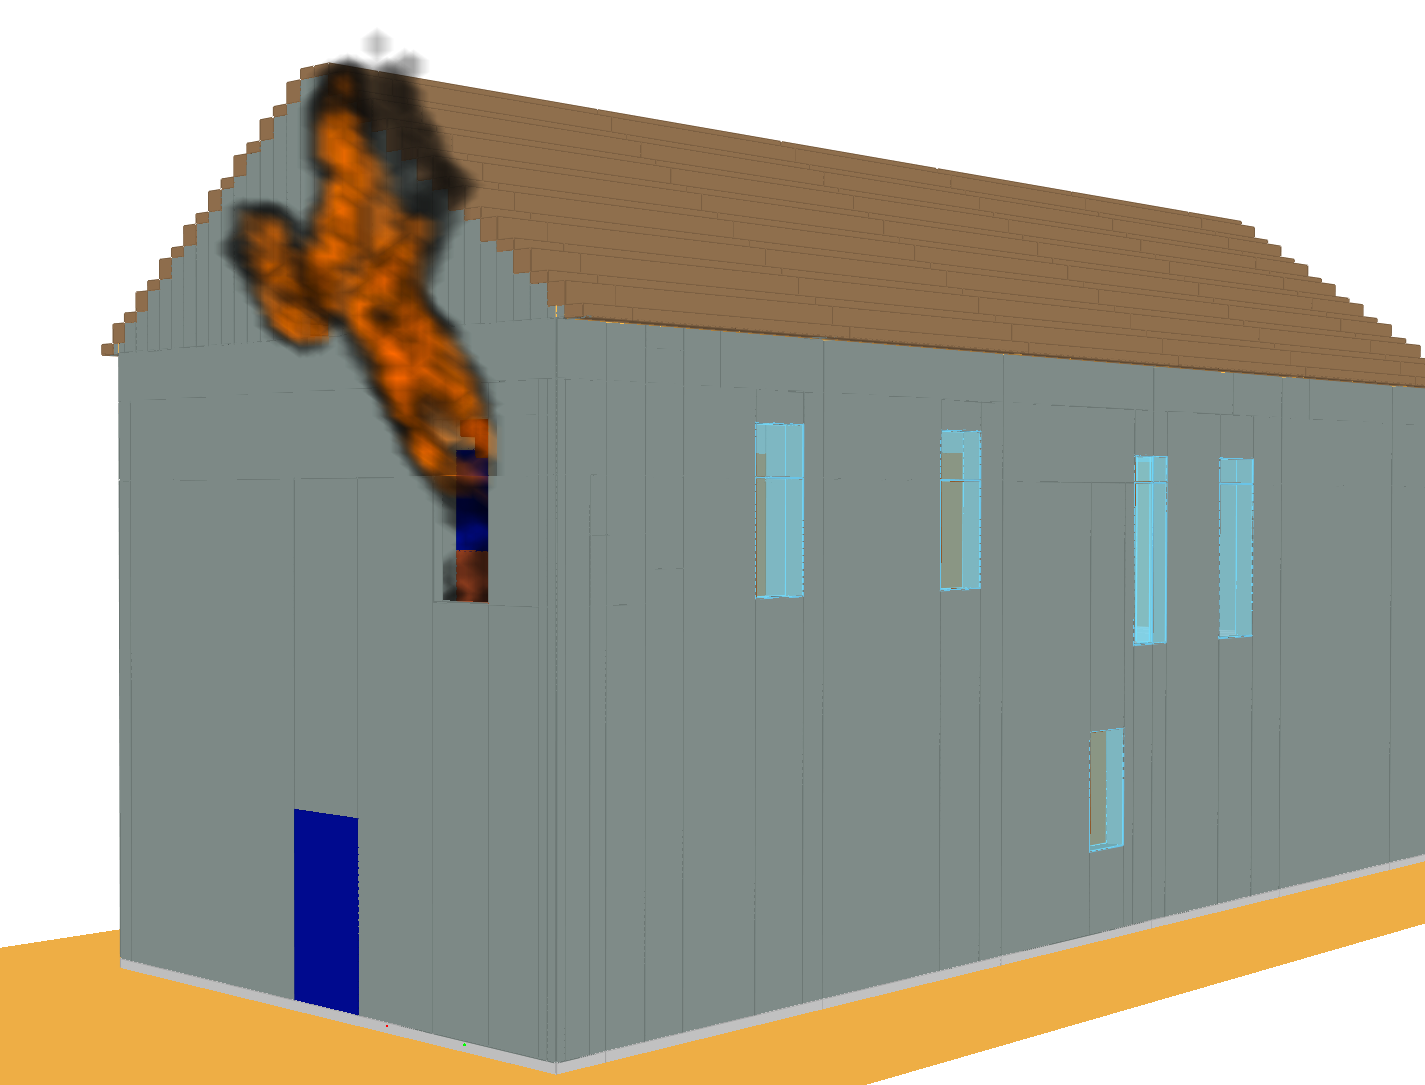
\includegraphics[width=.675\textwidth]{../Figures/smv_exterior_fire}
\caption{Smokeview rendering of exterior combustion occurring on the rear side of the structure.}
\label{fig:smv_ext_fire}
\end{figure}


\clearpage


\section{Pressure}

As the simulated fire grows in the attic and rear porch, the pressure rises. Figure~\ref{fig:pres_159s} shows the calculated pressure conditions in the structure just before the interior door failed in the simulation. On the rear porch, the pressure rise ranges from a 4~Pa ($5.8 \times 10^{-4}$~psi) over-pressure at a height of 1~m to greater than 10~Pa ($1.5 \times 10^{-3}$~psi) at the ceiling. Gases at an elevated pressure will always move towards a region of lower pressure. The door serves as a boundary between the high and low pressure regions. Once the door fails open, the high pressure gases flow towards the low pressure regions in the house, hallway, kitchen, and front stairwell. The velocity vectors shown in Fig.~\ref{fig:velo_175s} (15~s after the interior door fails) indicate the direction of flow within the structure.

\begin{figure}[!ht]
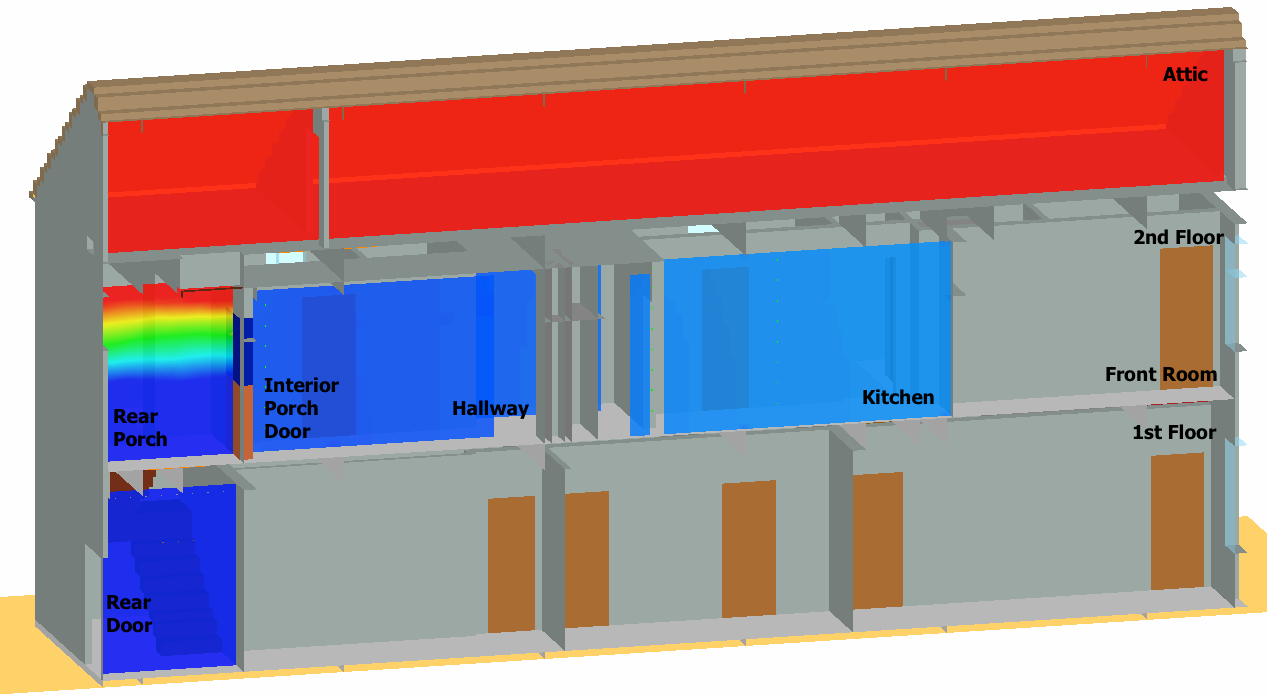
\includegraphics[width=.75\textwidth]{../Figures/west_50th_baseline_pres2}
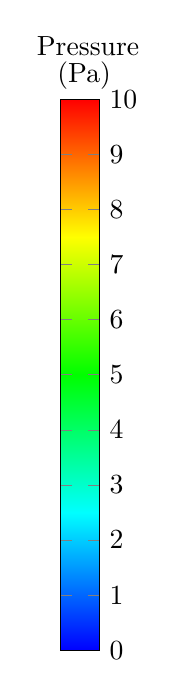
\begin{tikzpicture}
\pgfkeys{/pgf/number format/set thousands separator = {}}
\node at (0.65,0.67) {Pressure};
\node at (0.6,0.3) {(Pa)};
\begin{axis}[
    hide axis,
    scale only axis,
    height=0pt,
    width=0pt,
    colorbar,
    point meta min=0,
    point meta max=10,
    colorbar style={
        height=7cm,
        ytick={0,1,2,...,10}}
    ]
    \addplot [draw=none] coordinates {(0,0)};
\end{axis}
\end{tikzpicture}

\caption[FDS simulated pressure contours, 1~s prior to interior door failure.]{FDS simulated pressure contours, 1~s prior to interior door failure.}
\label{fig:pres_159s}
\end{figure}

\newpage
\begin{landscape}
\centering
\begin{figure}[!ht]
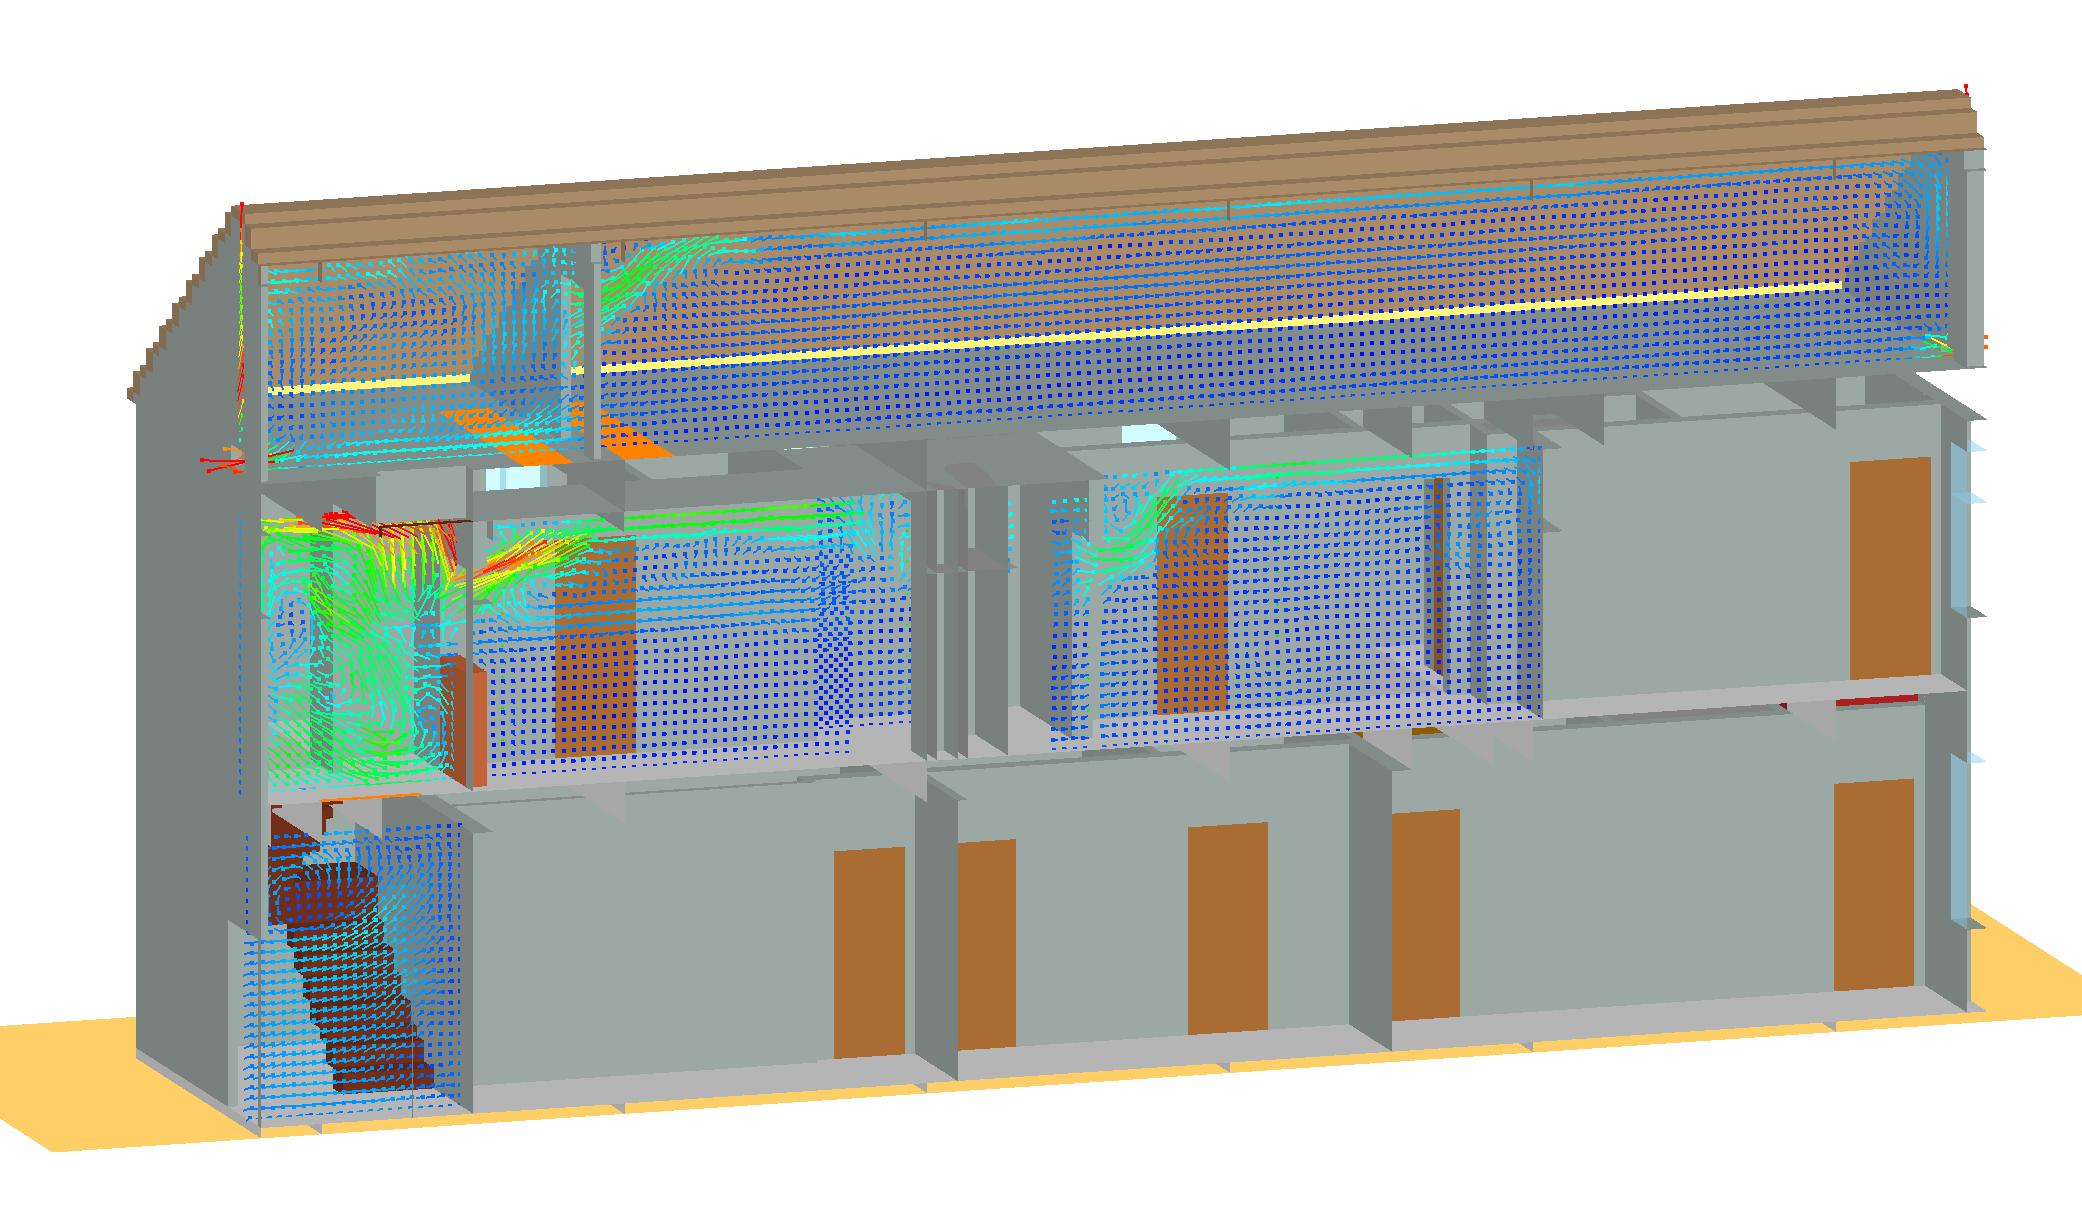
\includegraphics[width=1.1\textwidth]{../Figures/west_50th_baseline_velo_175}
%\documentclass{standalone}
%\usepackage{pgfplots}
%\begin{document}
%\pgfplotsset{
%	colormap={blackwhite}{[5pt]
%		rgb255(0pt)=(0,0,255); 
%		rgb255(100pt)=(0,255,255); 
%		rgb255(200pt)=(0,255,0); 
%		rgb255(300pt)=(255,255,0); 
%		rgb255(400pt)=(255,0,0)
%	},
%}
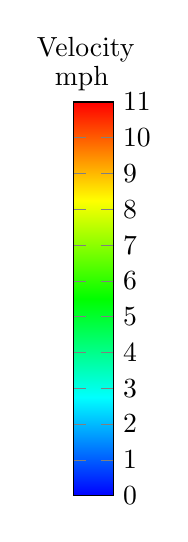
\begin{tikzpicture}
\node at (0.45,0.67) {Velocity};
\node at (0.4,0.3) {mph};
\begin{axis}[
    hide axis,
    scale only axis,
    height=0pt,
    width=0pt,
    colorbar,
    point meta min=0,
    point meta max=11,
    colorbar style={
        height=5cm,
        ytick={0,1,2,...,11}
    }]
    \addplot [draw=none] coordinates {(0,0)};
\end{axis}
\end{tikzpicture}
%\end{document}
%\documentclass{standalone}
%\usepackage{pgfplots}
%\begin{document}
%\pgfplotsset{
%	colormap={blackwhite}{[5pt]
%		rgb255(0pt)=(0,0,255); 
%		rgb255(100pt)=(0,255,255); 
%		rgb255(200pt)=(0,255,0); 
%		rgb255(300pt)=(255,255,0); 
%		rgb255(400pt)=(255,0,0)
%	},
%}
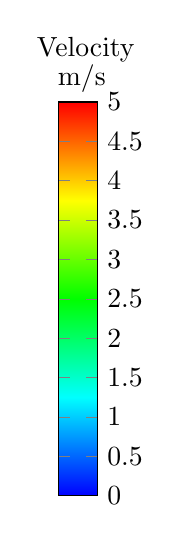
\begin{tikzpicture}
\node at (0.65,0.67) {Velocity};
\node at (0.6,0.3) {m/s};
\begin{axis}[
    hide axis,
    scale only axis,
    height=0pt,
    width=0pt,
    colorbar,
    point meta min=0,
    point meta max=5,
    colorbar style={
        height=5cm,
        ytick={0,0.5,1,...,5}
    }]
    \addplot [draw=none] coordinates {(0,0)};
\end{axis}
\end{tikzpicture}
%\end{document}

\caption{FDS simulated velocity vectors, 15~s after interior door failure.}
\label{fig:velo_175s}
\end{figure}
\end{landscape}
\newpage

\section{Temperature}
\label{temp}
Analysis of the temperatures from the FDS simulation focuses on the high hazard areas of the structure: the attic, the rear porch and stairwell, and the interior hallway which connects the rear porch to the front stairwell. The temperature profile at these high hazard areas is shown via several snapshots in time to illustrate the change in the interior conditions. The first snapshots are shown at a time of 129~s into the simulation, just before a firefighter opened the rear porch door (as shown in Fig.~\ref{fig:temp_129s}), and 159~s into the simulation, just before the interior door fails (as shown in Fig.~\ref{fig:temp_159s}).

\begin{figure}[!ht]
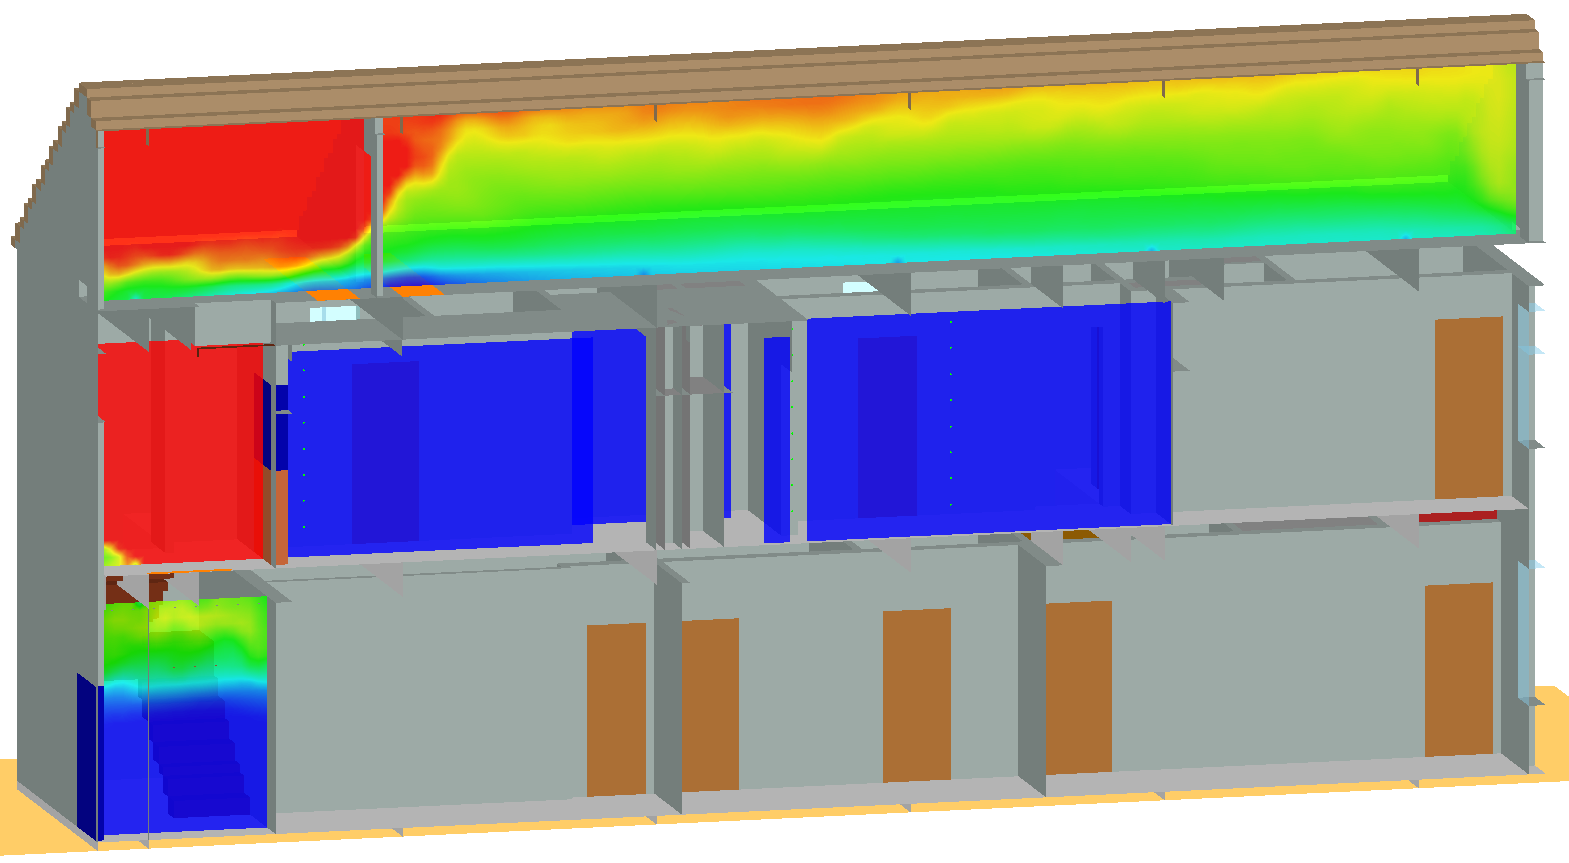
\includegraphics[width=.675\textwidth]{../Figures/west_50th_baseline_129}
%\documentclass{standalone}
%\usepackage{pgfplots}
%\begin{document}
%\pgfplotsset{
%	colormap={blackwhite}{[5pt]
%		rgb255(0pt)=(0,0,255); 
%		rgb255(100pt)=(0,255,255); 
%		rgb255(200pt)=(0,255,0); 
%		rgb255(300pt)=(255,255,0); 
%		rgb255(400pt)=(255,0,0)
%	},
%}
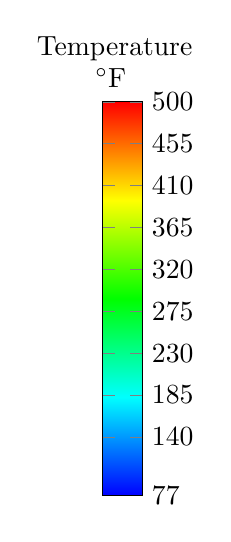
\begin{tikzpicture}
\node at (0.45,0.67) {Temperature};
\node at (0.4,0.3) {$^\circ$F};
\begin{axis}[
    hide axis,
    scale only axis,
    height=0pt,
    width=0pt,
    colorbar,
    point meta min=77,
    point meta max=500,
    colorbar style={
        height=5cm,
        ytick={77,140,185,...,500}
    }]
    \addplot [draw=none] coordinates {(0,0)};
\end{axis}
\end{tikzpicture}
%\end{document} 
%\documentclass{standalone}
%\usepackage{pgfplots}
%\begin{document}
%\pgfplotsset{
%	colormap={blackwhite}{[5pt]
%		rgb255(0pt)=(0,0,255); 
%		rgb255(100pt)=(0,255,255); 
%		rgb255(200pt)=(0,255,0); 
%		rgb255(300pt)=(255,255,0); 
%		rgb255(400pt)=(255,0,0)
%	},
%}
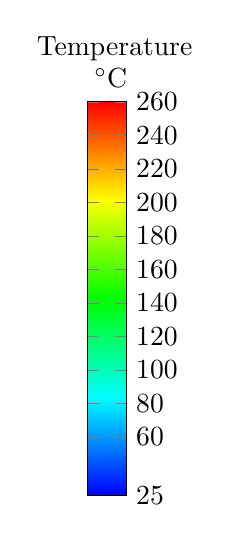
\begin{tikzpicture}
\node at (0.65,0.67) {Temperature};
\node at (0.6,0.3) {$^\circ$C};
\begin{axis}[
    hide axis,
    scale only axis,
    height=0pt,
    width=0pt,
    colorbar,
    point meta min=25,
    point meta max=260,
    colorbar style={
        height=5cm,
        ytick={25,60,80,...,260}
    }]
    \addplot [draw=none] coordinates {(0,0)};
\end{axis}
\end{tikzpicture}
%\end{document}

\caption{FDS simulated temperature contours, 1~s prior to rear door opening.}
\label{fig:temp_129s}
\end{figure}

\begin{figure}[!ht]
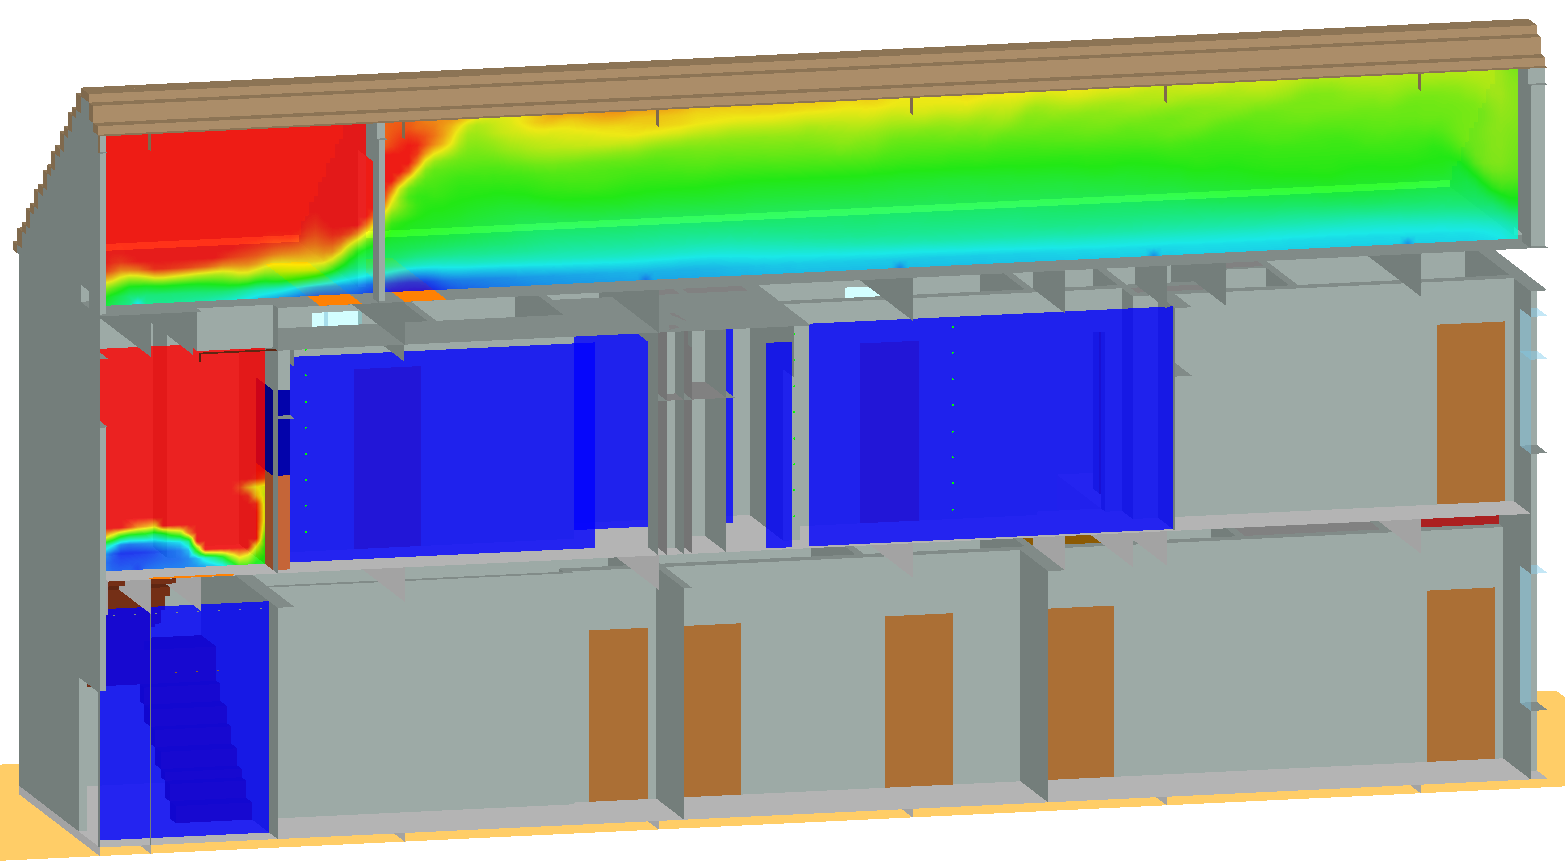
\includegraphics[width=.675\textwidth]{../Figures/west_50th_baseline_159}
%\documentclass{standalone}
%\usepackage{pgfplots}
%\begin{document}
%\pgfplotsset{
%	colormap={blackwhite}{[5pt]
%		rgb255(0pt)=(0,0,255); 
%		rgb255(100pt)=(0,255,255); 
%		rgb255(200pt)=(0,255,0); 
%		rgb255(300pt)=(255,255,0); 
%		rgb255(400pt)=(255,0,0)
%	},
%}
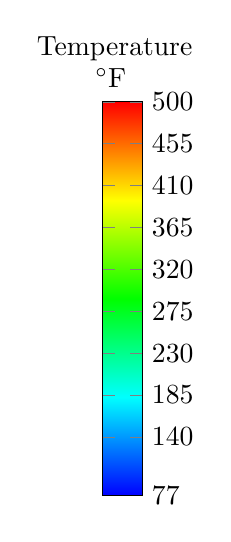
\begin{tikzpicture}
\node at (0.45,0.67) {Temperature};
\node at (0.4,0.3) {$^\circ$F};
\begin{axis}[
    hide axis,
    scale only axis,
    height=0pt,
    width=0pt,
    colorbar,
    point meta min=77,
    point meta max=500,
    colorbar style={
        height=5cm,
        ytick={77,140,185,...,500}
    }]
    \addplot [draw=none] coordinates {(0,0)};
\end{axis}
\end{tikzpicture}
%\end{document} 
%\documentclass{standalone}
%\usepackage{pgfplots}
%\begin{document}
%\pgfplotsset{
%	colormap={blackwhite}{[5pt]
%		rgb255(0pt)=(0,0,255); 
%		rgb255(100pt)=(0,255,255); 
%		rgb255(200pt)=(0,255,0); 
%		rgb255(300pt)=(255,255,0); 
%		rgb255(400pt)=(255,0,0)
%	},
%}
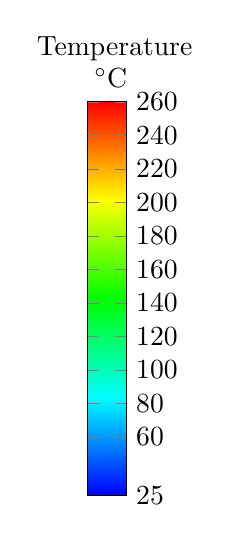
\begin{tikzpicture}
\node at (0.65,0.67) {Temperature};
\node at (0.6,0.3) {$^\circ$C};
\begin{axis}[
    hide axis,
    scale only axis,
    height=0pt,
    width=0pt,
    colorbar,
    point meta min=25,
    point meta max=260,
    colorbar style={
        height=5cm,
        ytick={25,60,80,...,260}
    }]
    \addplot [draw=none] coordinates {(0,0)};
\end{axis}
\end{tikzpicture}
%\end{document}

\caption{FDS simulated temperature contours, 1~s prior to interior door failure.}
\label{fig:temp_159s}
\end{figure}

Figure~\ref{fig:temp_129s} shows temperatures of at least 260~$^{\circ}$C (500~$^{\circ}$F) in the second floor rear porch and rear portion of the attic. High temperatures, between 80~$^{\circ}$C (185~$^{\circ}$F) and 200~$^{\circ}$C (390~$^{\circ}$F), also extend down to the rear entrance on the first floor. Before the interior door fails (Fig.~\ref{fig:temp_159s}), the inflow of ambient air from the open rear door reduces the temperatures near the interior doorway, but at the same time, the HRR increases because of the additional ventilation, as shown in Fig.~\ref{fig:hrr}. As shown in Fig.~\ref{fig:temp_161s}, after the second floor interior door fails, the high temperature gas that filled the rear porch flows in the direction of lower pressure (i.e., towards the front door). Note that the conditions in the attic do not appear to change.
\begin{figure}[!ht]
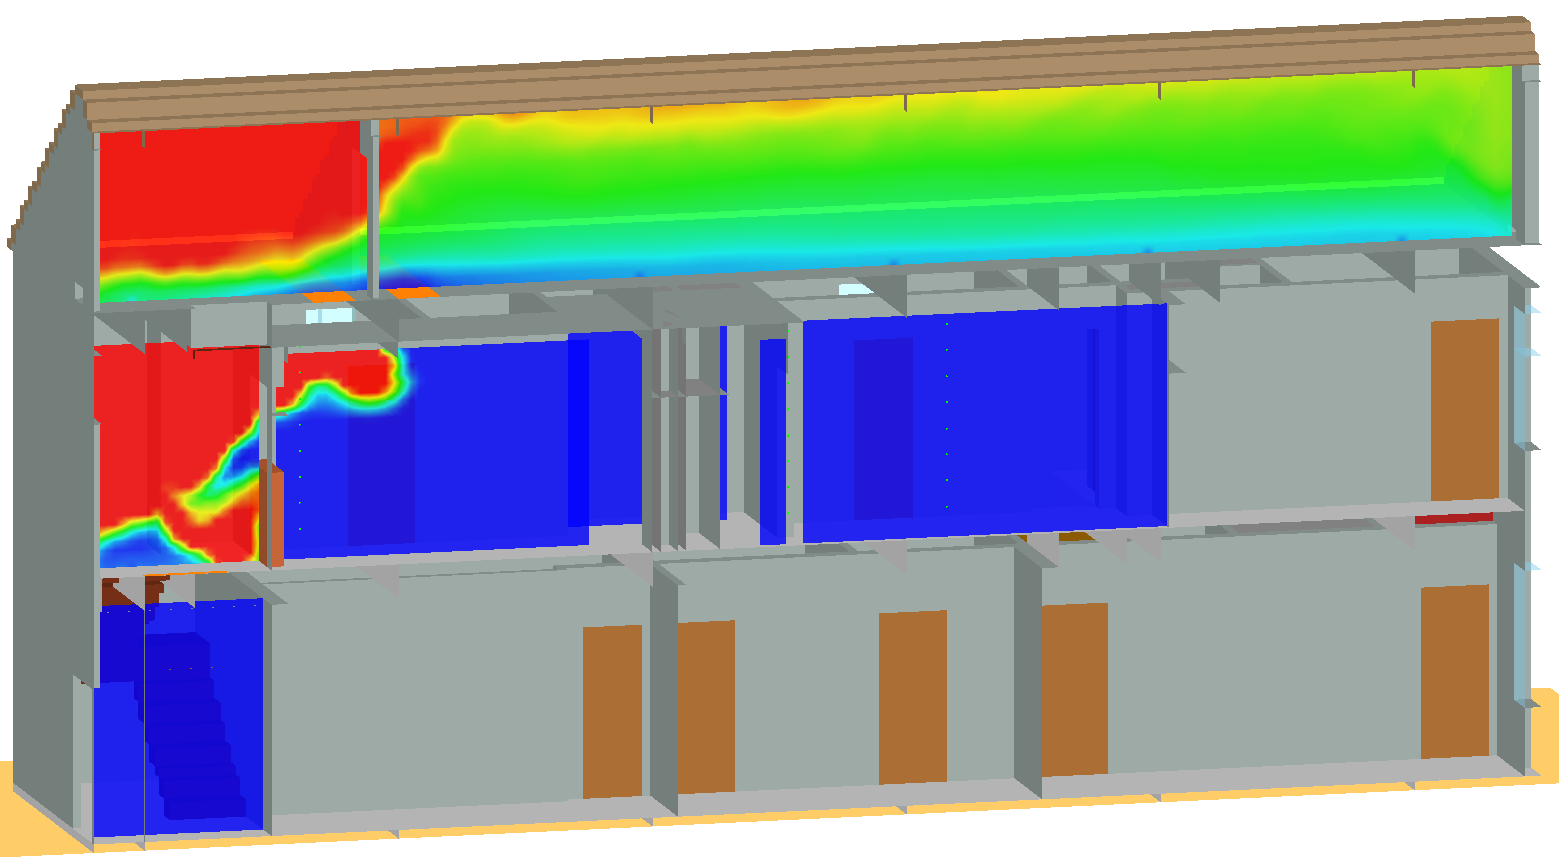
\includegraphics[width=.675\textwidth]{../Figures/west_50th_baseline_161}
%\documentclass{standalone}
%\usepackage{pgfplots}
%\begin{document}
%\pgfplotsset{
%	colormap={blackwhite}{[5pt]
%		rgb255(0pt)=(0,0,255); 
%		rgb255(100pt)=(0,255,255); 
%		rgb255(200pt)=(0,255,0); 
%		rgb255(300pt)=(255,255,0); 
%		rgb255(400pt)=(255,0,0)
%	},
%}
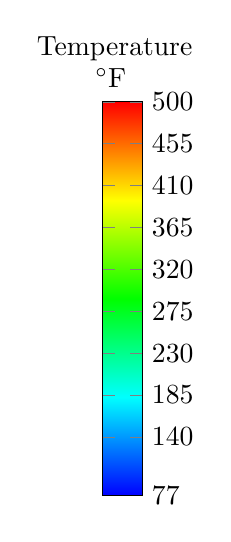
\begin{tikzpicture}
\node at (0.45,0.67) {Temperature};
\node at (0.4,0.3) {$^\circ$F};
\begin{axis}[
    hide axis,
    scale only axis,
    height=0pt,
    width=0pt,
    colorbar,
    point meta min=77,
    point meta max=500,
    colorbar style={
        height=5cm,
        ytick={77,140,185,...,500}
    }]
    \addplot [draw=none] coordinates {(0,0)};
\end{axis}
\end{tikzpicture}
%\end{document} 
%\documentclass{standalone}
%\usepackage{pgfplots}
%\begin{document}
%\pgfplotsset{
%	colormap={blackwhite}{[5pt]
%		rgb255(0pt)=(0,0,255); 
%		rgb255(100pt)=(0,255,255); 
%		rgb255(200pt)=(0,255,0); 
%		rgb255(300pt)=(255,255,0); 
%		rgb255(400pt)=(255,0,0)
%	},
%}
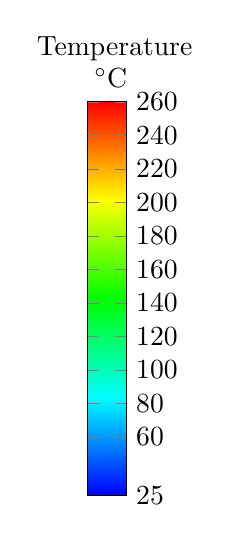
\begin{tikzpicture}
\node at (0.65,0.67) {Temperature};
\node at (0.6,0.3) {$^\circ$C};
\begin{axis}[
    hide axis,
    scale only axis,
    height=0pt,
    width=0pt,
    colorbar,
    point meta min=25,
    point meta max=260,
    colorbar style={
        height=5cm,
        ytick={25,60,80,...,260}
    }]
    \addplot [draw=none] coordinates {(0,0)};
\end{axis}
\end{tikzpicture}
%\end{document}

\caption{FDS simulated temperature contours, 1~s after interior door failure.}
\label{fig:temp_161s}
\end{figure}

\begin{figure}[!ht]
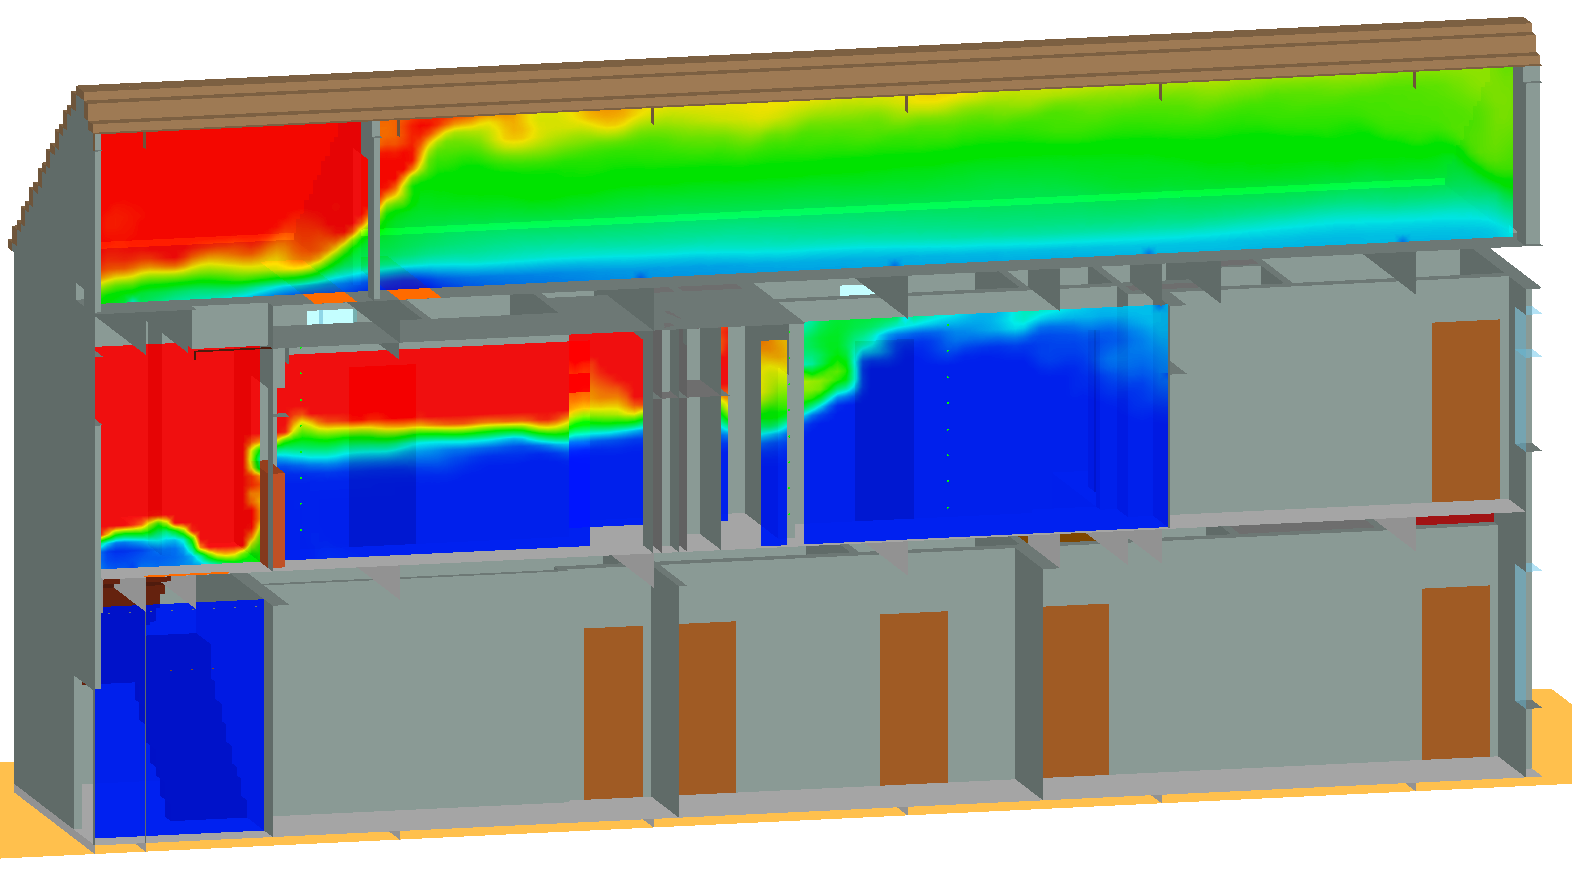
\includegraphics[width=.675\textwidth]{../Figures/west_50th_baseline_175}
%\documentclass{standalone}
%\usepackage{pgfplots}
%\begin{document}
%\pgfplotsset{
%	colormap={blackwhite}{[5pt]
%		rgb255(0pt)=(0,0,255); 
%		rgb255(100pt)=(0,255,255); 
%		rgb255(200pt)=(0,255,0); 
%		rgb255(300pt)=(255,255,0); 
%		rgb255(400pt)=(255,0,0)
%	},
%}
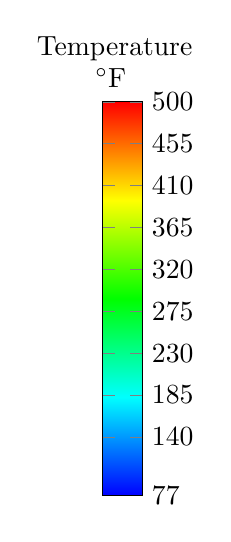
\begin{tikzpicture}
\node at (0.45,0.67) {Temperature};
\node at (0.4,0.3) {$^\circ$F};
\begin{axis}[
    hide axis,
    scale only axis,
    height=0pt,
    width=0pt,
    colorbar,
    point meta min=77,
    point meta max=500,
    colorbar style={
        height=5cm,
        ytick={77,140,185,...,500}
    }]
    \addplot [draw=none] coordinates {(0,0)};
\end{axis}
\end{tikzpicture}
%\end{document} 
%\documentclass{standalone}
%\usepackage{pgfplots}
%\begin{document}
%\pgfplotsset{
%	colormap={blackwhite}{[5pt]
%		rgb255(0pt)=(0,0,255); 
%		rgb255(100pt)=(0,255,255); 
%		rgb255(200pt)=(0,255,0); 
%		rgb255(300pt)=(255,255,0); 
%		rgb255(400pt)=(255,0,0)
%	},
%}
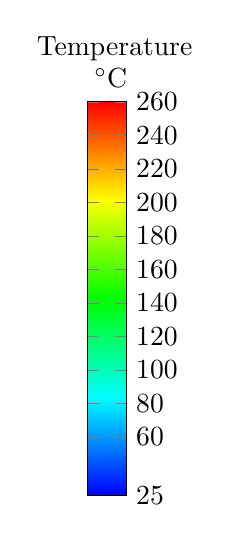
\begin{tikzpicture}
\node at (0.65,0.67) {Temperature};
\node at (0.6,0.3) {$^\circ$C};
\begin{axis}[
    hide axis,
    scale only axis,
    height=0pt,
    width=0pt,
    colorbar,
    point meta min=25,
    point meta max=260,
    colorbar style={
        height=5cm,
        ytick={25,60,80,...,260}
    }]
    \addplot [draw=none] coordinates {(0,0)};
\end{axis}
\end{tikzpicture}
%\end{document}

\caption{FDS simulated temperature contours, 15~s after the interior door failure.}
\label{fig:temp_175s}
\end{figure}

As shown in Fig.~\ref{fig:temp_175s}, 15~s after the door failed, high temperature gases descended to approximately 1~m (3.28~ft) above the floor through the interior hallway and are flowing into the kitchen.


\chapter{Discussion of Simulation Results}
\label{discussion}
The results of the FDS simulations are discussed in the following two sections. The first section addresses the results of the computational modeling as they relate to the interior hallways conditions. The second section examines the model results and observed outcomes of the fire incident as they relate to tactics discussed in recent experimental research. 

\section{Simulated Hallway Flow Path}
From on-scene reports (Section~\ref{fire_sum}) and the FDS simulation results (Section~\ref{temp}), the interior conditions on the second floor of the structure were initially tenable. From the NIOSH report~\cite{NIOSH:Bowyer}, while the IC was inside the structure on the second floor, only light haze and a glow around the door between the hallway and enclosed porch was observed. This indicated the presence of fire in the area of the enclosed porch. The simulation results indicate a high hazard area (temperatures greater than 260~$^{\circ}$C or 500~$^{\circ}$F) in the attic and the enclosed porch at this time. By the time the E123 captain and firefighter arrived on the second floor (Table~\ref{tab:firesim}) and approached the rear of the structure, the rear porch was fully involved. Temperature conditions greater than 260~$^{\circ}$C (500~$^{\circ}$F) were present on the porch side of the steel-faced, wood-framed door at the rear of the structure. Exposure to these conditions likely weakened the structural integrity of the door, which may have led to a partial failure (Table~\ref{tab:firesim}). Figure~\ref{fig:chicago_doorfold} shows the state of the rear door after the fire. Note the large crease in the steel face of the door just above the knob.

\begin{figure}[!ht]
\centering
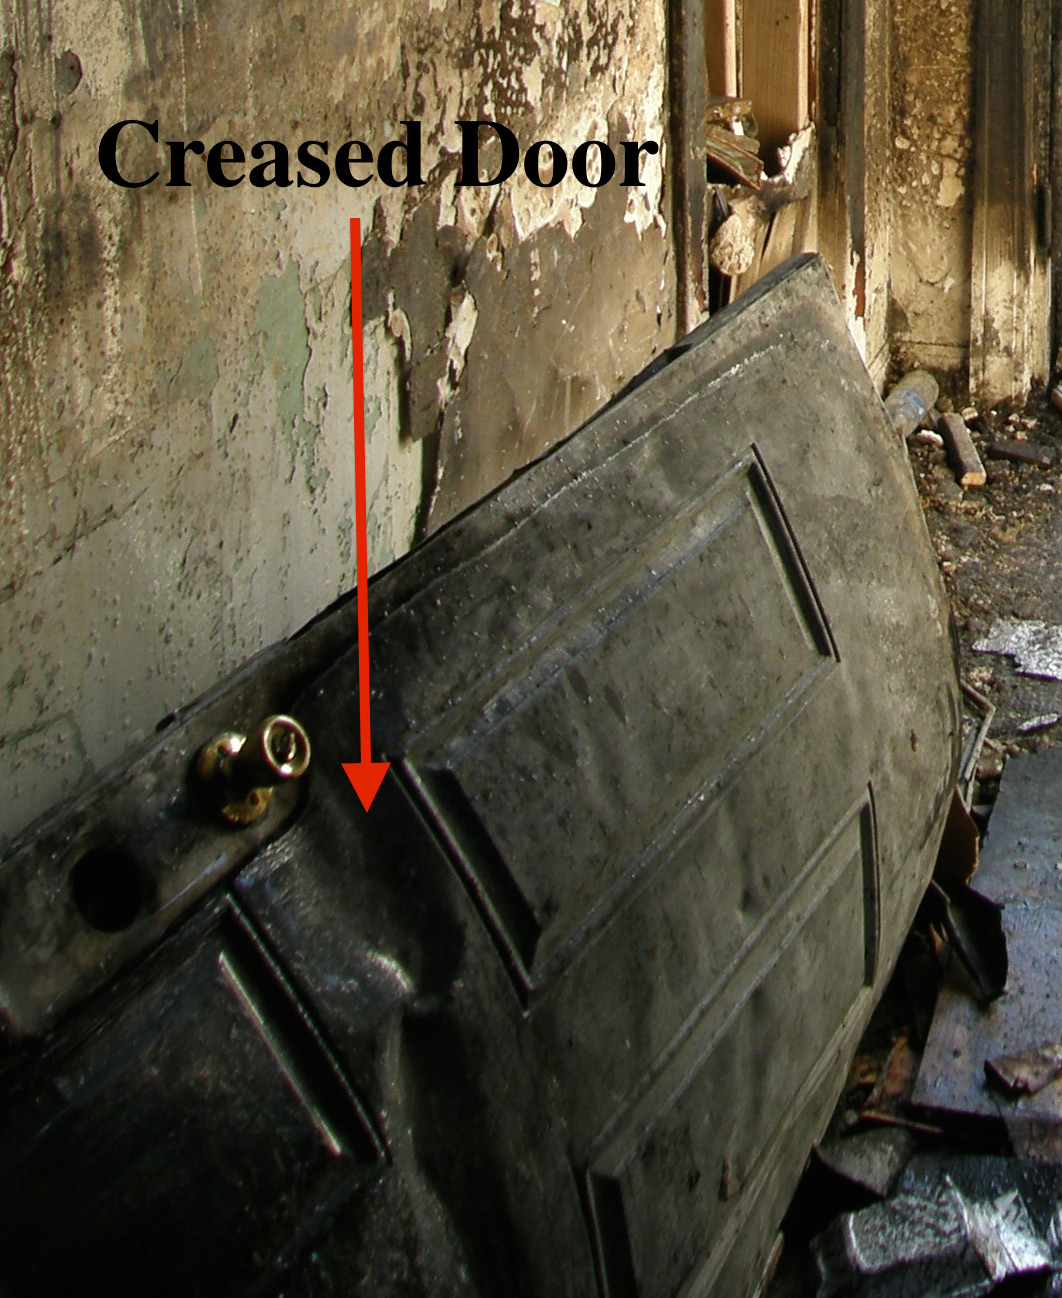
\includegraphics[width=.4\textwidth]{../Figures/Porch_Door_1}
\caption{Post-fire image of interior door.}
\label{fig:chicago_doorfold}
\end{figure}

Recent experiments conducted by NIST revealed similar post-fire states after doors of similar construction were exposed to fires. Figure~\ref{fig:SC_doorfold} shows doors from two different residential fire experiments in different stages of degradation. In both cases, note that the door knob assembly served as a pivot point for the upper portion of the door to collapse around. This is similar to the location of the creases in the remains of the steel door that was located between the hallway and the enclosed porch in this fire incident.

\begin{figure}[!ht]
\centering
\begin{tabular*}{\textwidth}{l@{\extracolsep{\fill}}r}
   \scalebox{1.0}{ 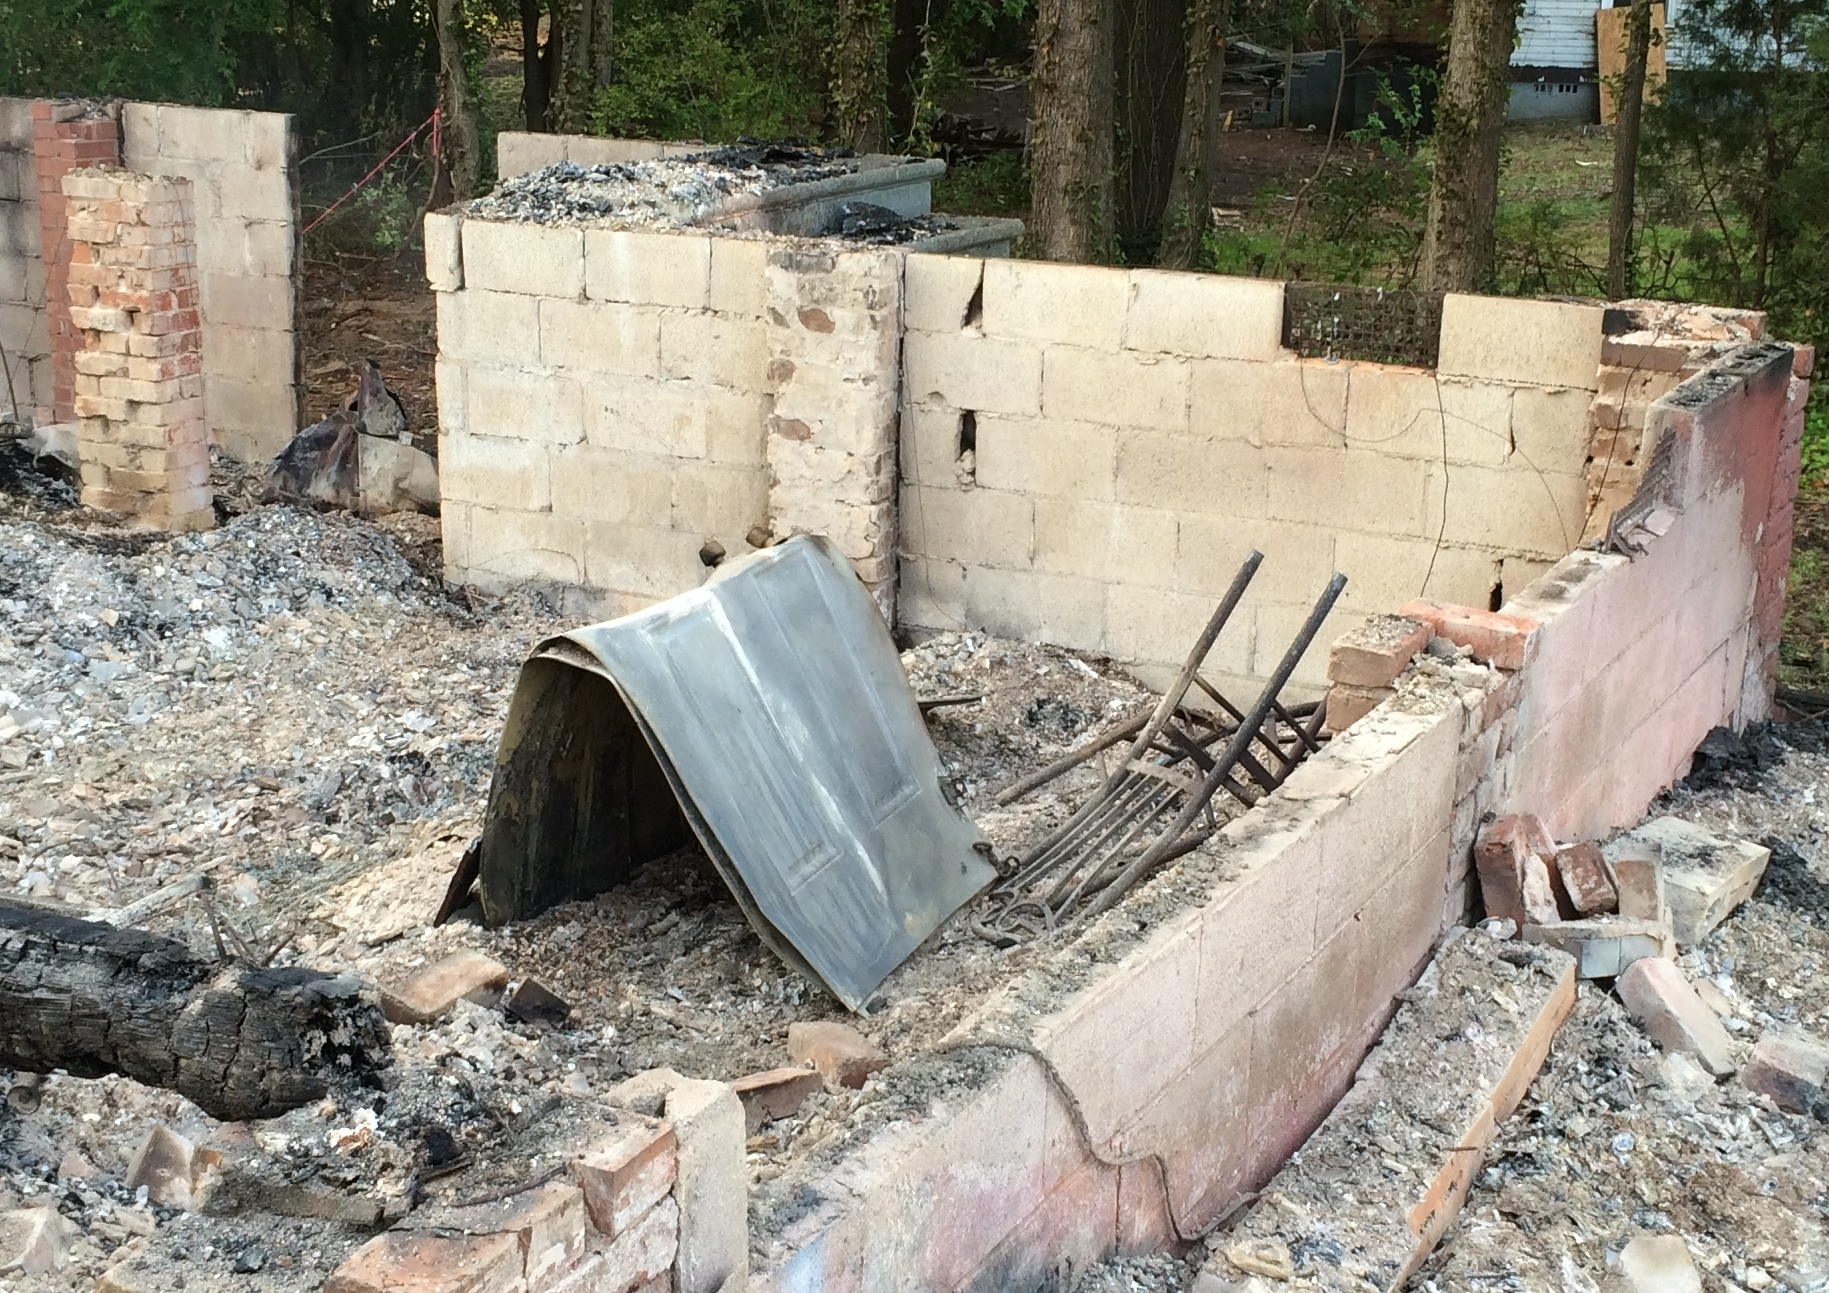
\includegraphics[width=3in]{../Figures/SC_Door_1} } &
   \scalebox{1.0}{ 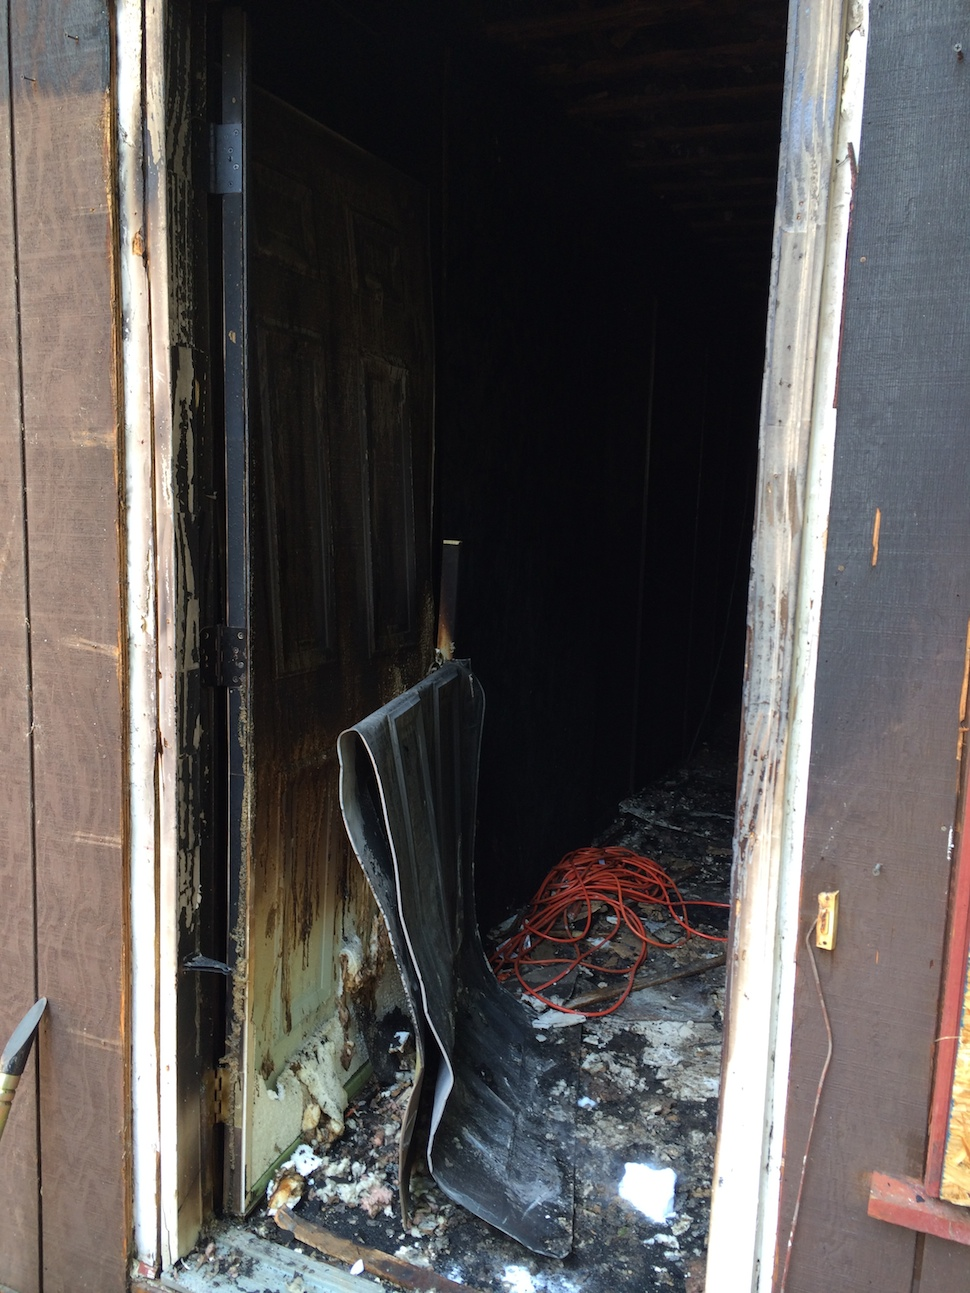
\includegraphics[width=2in]{../Figures/SC_Door_2} } \\
\end{tabular*}
\caption{Post-experiment images of door failures.}
\label{fig:SC_doorfold}
\end{figure}

After the interior door failed, an interior flow path was created from the enclosed porch area into the kitchen of the structure. This resulted in a rapid change in the conditions within the flow path. The combustion gases at elevated temperature and pressure in the enclosed porch were vented by the failure of the door and flowed towards lower pressure areas in the hallways and kitchen. The arrows shown in Fig.~\ref{fig:flowpath_1} summarize the simulated flow direction of gases on the second floor after the door failure. In this figure, the red arrows indicate elevated gas temperatures, and the blue arrows indicate relatively cooler gas temperatures. The arrow that transitions from red to blue indicates that the heated gases were cooling as they flowed away from the fire towards the front of the structure. The two arrows located at the door on the second floor (towards the front of the structure) indicate bi-directional flow. At that doorway, cool ambient air flowed towards the fire near the bottom of the door, and hot gases flowed away from the fire near the top of the door.

\begin{figure}[!ht]
\centering
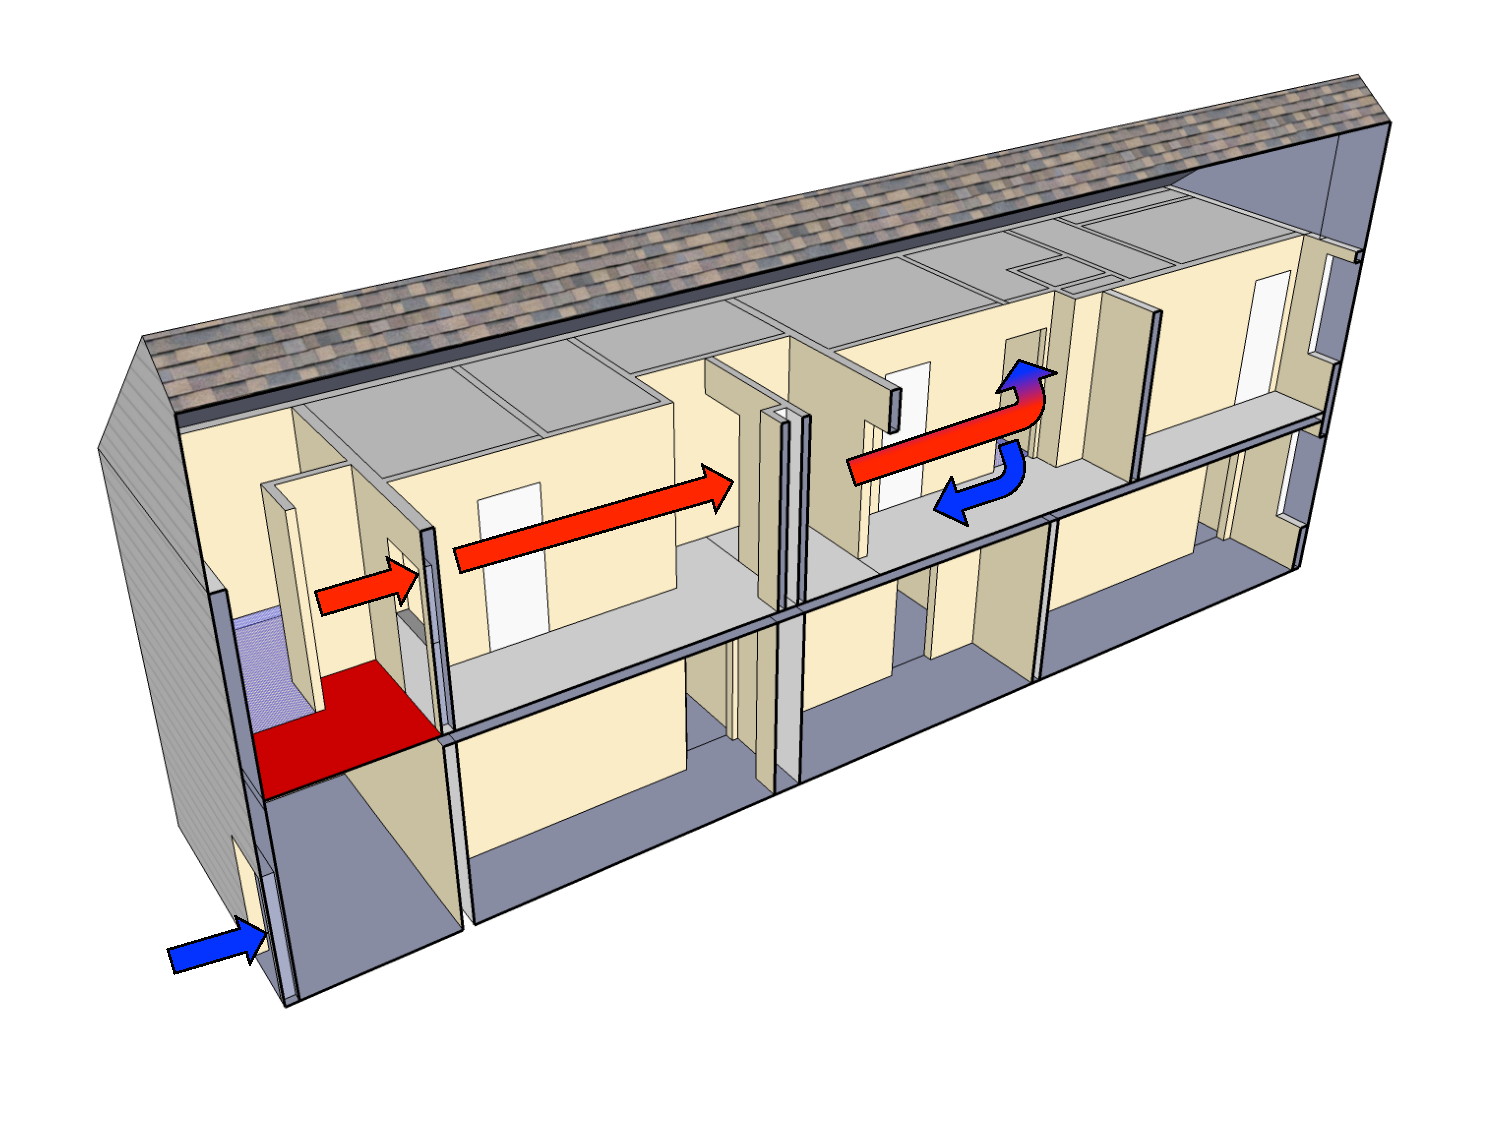
\includegraphics[width=.7\textwidth]{../Figures/ChicagoFlow}
\caption{Summary of simulated flow path on the second floor after interior door failure.}
\label{fig:flowpath_1}
\end{figure}


\clearpage


\section{Assessing the Hazard}

A person is susceptible to second-degree burn injuries if exposed to temperatures greater than 55~$^{\circ}$C (130~$^{\circ}$F)~\cite{contactburn}. Although firefighters wear protective gear, gear only offers a finite amount of protection. The polycarbonate in a self contained breathing apparatus begins to soften when the material temperature reaches approximately 140~$^{\circ}$C (284~$^{\circ}$F)~\cite{mensch2011emergency}. Structural fire fighting coats and pants are tested to withstand temperatures of 260~$^{\circ}$C (500~$^{\circ}$F)~\cite{nfpa2013standard}. Prolonged exposure to elevated temperatures can result in a significant amount of heat transferred to the firefighter, putting him/her at risk. Exposure of equipment to temperatures of 260~$^{\circ}$C (500~$^{\circ}$F) represents a Class III exposure~\cite{Donnelly2006}. Firefighters are at increased risk levels when encountering Class III exposure conditions for more than 5~minutes~\cite{Donnelly2006}. Therefore, for the analysis of the simulated exposure temperatures, the maximum visualized temperature is set to indicate all values that are greater than or equal to 260~$^{\circ}$C (500~$^{\circ}$F). This means that temperatures visualized at the maximum range in the displayed model output are at a minimum of 260~$^{\circ}$C (500~$^{\circ}$F); the actual simulated temperatures could in fact be greater. 

Prior to the interior door failure, the elevated temperatures on the second floor were limited to the rear porch, as shown in Fig.~\ref{fig:temp_top_159}. The temperatures were greatest at the back-left corner where there is sufficient oxygen due to the section of porch wall that had burned away and allowed additional oxygen to mix with the fuel-rich fire gases. Five seconds after the interior door failed, hot gases traveled the length of the interior hallway and approached the doorway into the kitchen, which was approximately 4.5~m (14.8~ft) away from the source fire, as shown in Fig.~\ref{fig:temp_top_165}. Within 60~s of the interior door failure, the hallway temperatures were approximately at or above 260~$^{\circ}$C (500~$^{\circ}$F) throughout the hallway, as shown in Fig.~\ref{fig:temp_top_220}. These results indicate that the high temperature gases seen 5~s after failure were not just a burst but rather the front of a sustained exhaust gas flow from the fire burning in the enclosed rear porch. The conditions in this hallway changed from tenable to high-hazard very rapidly following the door failure. Figure~\ref{fig:temp_top_220} also shows that the temperatures in the kitchen were at or below 90~$^{\circ}$C (194~$^{\circ}$F), and the temperatures at the top of the stairs were at or below 70~$^{\circ}$C (158~$^{\circ}$F). At these locations within the structure, the exhaust gases in the flow path were cooled and diluted by the inflowing ambient gas. These simulated temperatures are consistent with the post-incident conditions that were documented in the kitchen and second floor stairwell.

\begin{figure}[!ht]
\centering
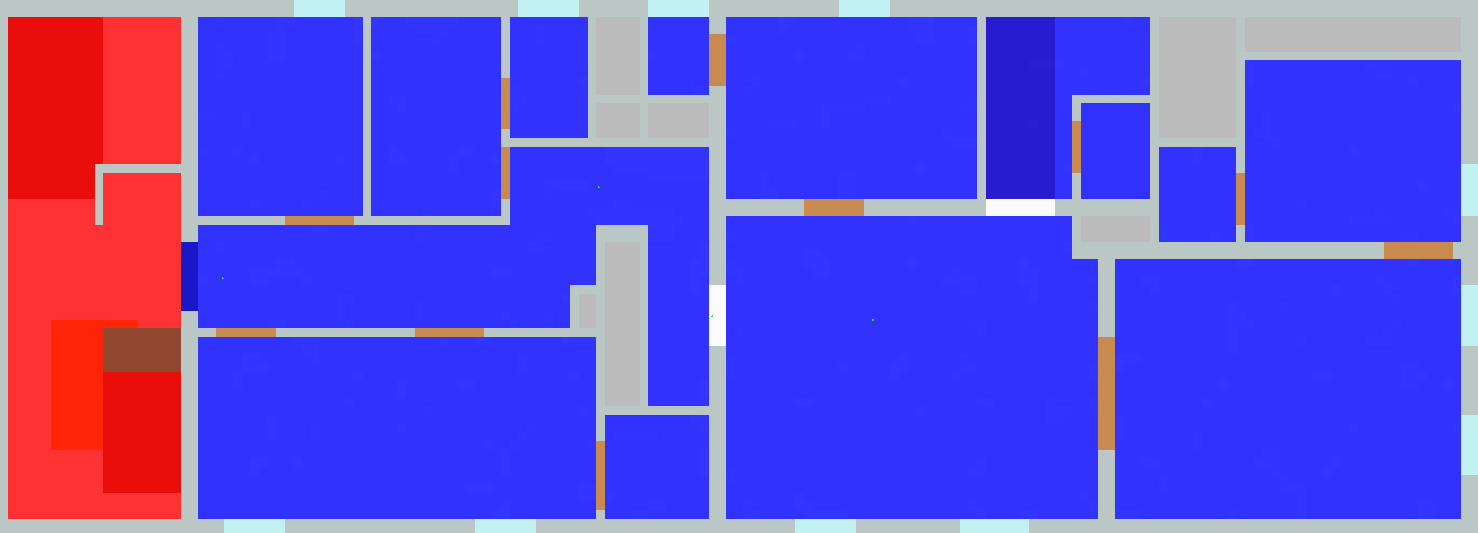
\includegraphics[width=.68\textwidth]{../Figures/west_50th_baseline_top_159_6ft}
%\documentclass{standalone}
%\usepackage{pgfplots}
%\begin{document}
%\pgfplotsset{
%	colormap={blackwhite}{[5pt]
%		rgb255(0pt)=(0,0,255); 
%		rgb255(100pt)=(0,255,255); 
%		rgb255(200pt)=(0,255,0); 
%		rgb255(300pt)=(255,255,0); 
%		rgb255(400pt)=(255,0,0)
%	},
%}
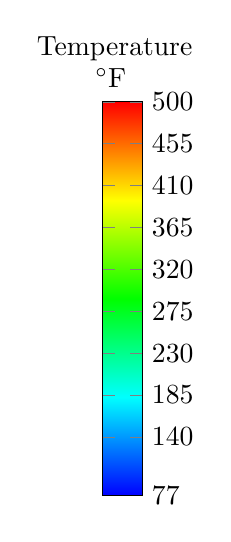
\begin{tikzpicture}
\node at (0.45,0.67) {Temperature};
\node at (0.4,0.3) {$^\circ$F};
\begin{axis}[
    hide axis,
    scale only axis,
    height=0pt,
    width=0pt,
    colorbar,
    point meta min=77,
    point meta max=500,
    colorbar style={
        height=5cm,
        ytick={77,140,185,...,500}
    }]
    \addplot [draw=none] coordinates {(0,0)};
\end{axis}
\end{tikzpicture}
%\end{document} 
%\documentclass{standalone}
%\usepackage{pgfplots}
%\begin{document}
%\pgfplotsset{
%	colormap={blackwhite}{[5pt]
%		rgb255(0pt)=(0,0,255); 
%		rgb255(100pt)=(0,255,255); 
%		rgb255(200pt)=(0,255,0); 
%		rgb255(300pt)=(255,255,0); 
%		rgb255(400pt)=(255,0,0)
%	},
%}
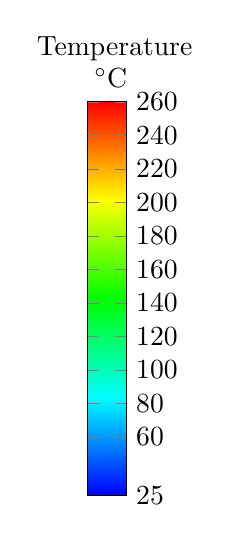
\begin{tikzpicture}
\node at (0.65,0.67) {Temperature};
\node at (0.6,0.3) {$^\circ$C};
\begin{axis}[
    hide axis,
    scale only axis,
    height=0pt,
    width=0pt,
    colorbar,
    point meta min=25,
    point meta max=260,
    colorbar style={
        height=5cm,
        ytick={25,60,80,...,260}
    }]
    \addplot [draw=none] coordinates {(0,0)};
\end{axis}
\end{tikzpicture}
%\end{document}

\caption[Temperature contours on the second floor, 1~s prior to interior door failure.]
{Temperature contours on the second floor, 1~s prior to interior door failure, 1.83~m (6~ft) above the floor.}
\label{fig:temp_top_159}
\end{figure}

\begin{figure}[!ht]
\centering
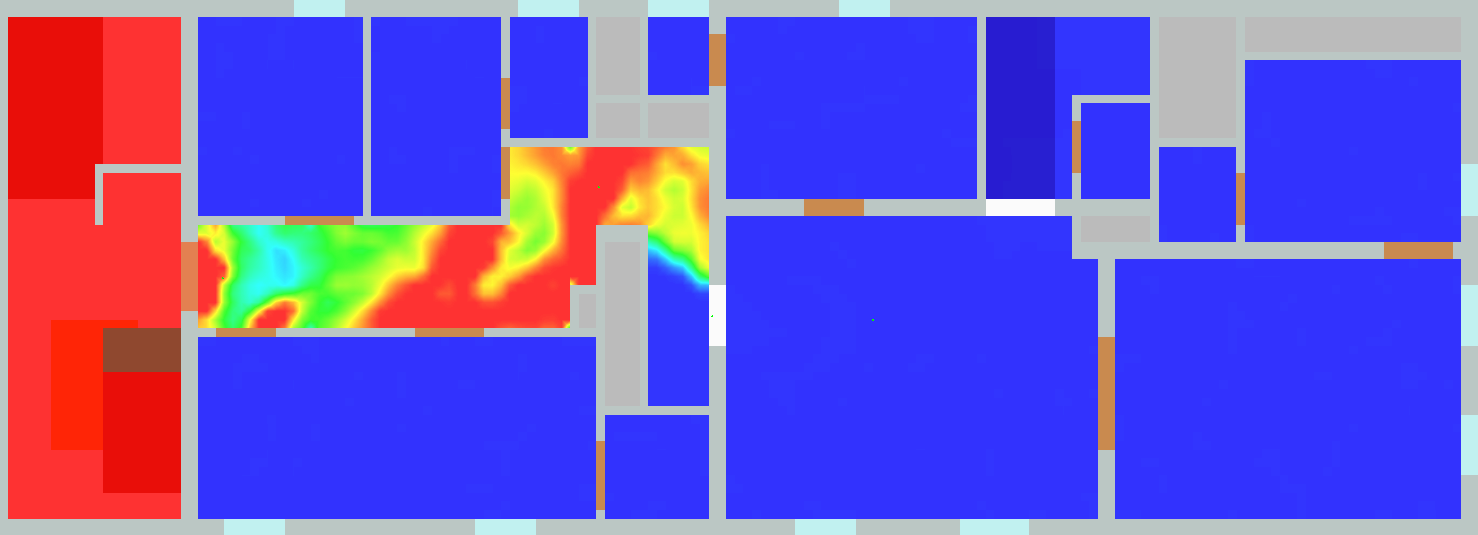
\includegraphics[width=.68\textwidth]{../Figures/west_50th_baseline_top_165_6ft}
%\documentclass{standalone}
%\usepackage{pgfplots}
%\begin{document}
%\pgfplotsset{
%	colormap={blackwhite}{[5pt]
%		rgb255(0pt)=(0,0,255); 
%		rgb255(100pt)=(0,255,255); 
%		rgb255(200pt)=(0,255,0); 
%		rgb255(300pt)=(255,255,0); 
%		rgb255(400pt)=(255,0,0)
%	},
%}
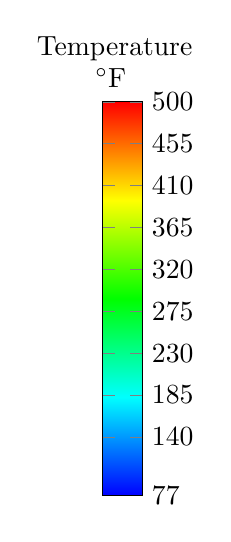
\begin{tikzpicture}
\node at (0.45,0.67) {Temperature};
\node at (0.4,0.3) {$^\circ$F};
\begin{axis}[
    hide axis,
    scale only axis,
    height=0pt,
    width=0pt,
    colorbar,
    point meta min=77,
    point meta max=500,
    colorbar style={
        height=5cm,
        ytick={77,140,185,...,500}
    }]
    \addplot [draw=none] coordinates {(0,0)};
\end{axis}
\end{tikzpicture}
%\end{document} 
%\documentclass{standalone}
%\usepackage{pgfplots}
%\begin{document}
%\pgfplotsset{
%	colormap={blackwhite}{[5pt]
%		rgb255(0pt)=(0,0,255); 
%		rgb255(100pt)=(0,255,255); 
%		rgb255(200pt)=(0,255,0); 
%		rgb255(300pt)=(255,255,0); 
%		rgb255(400pt)=(255,0,0)
%	},
%}
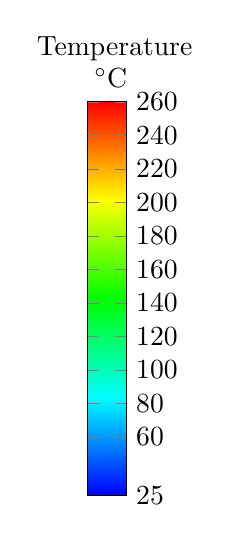
\begin{tikzpicture}
\node at (0.65,0.67) {Temperature};
\node at (0.6,0.3) {$^\circ$C};
\begin{axis}[
    hide axis,
    scale only axis,
    height=0pt,
    width=0pt,
    colorbar,
    point meta min=25,
    point meta max=260,
    colorbar style={
        height=5cm,
        ytick={25,60,80,...,260}
    }]
    \addplot [draw=none] coordinates {(0,0)};
\end{axis}
\end{tikzpicture}
%\end{document}

\caption[Temperature contours on the second floor, 5~s after interior door failure.]
{Temperature contours on the second floor, 5~s after interior door failure, 1.83~m (6~ft) above the floor.}
\label{fig:temp_top_165}
\end{figure}

\begin{figure}[!ht]
\centering
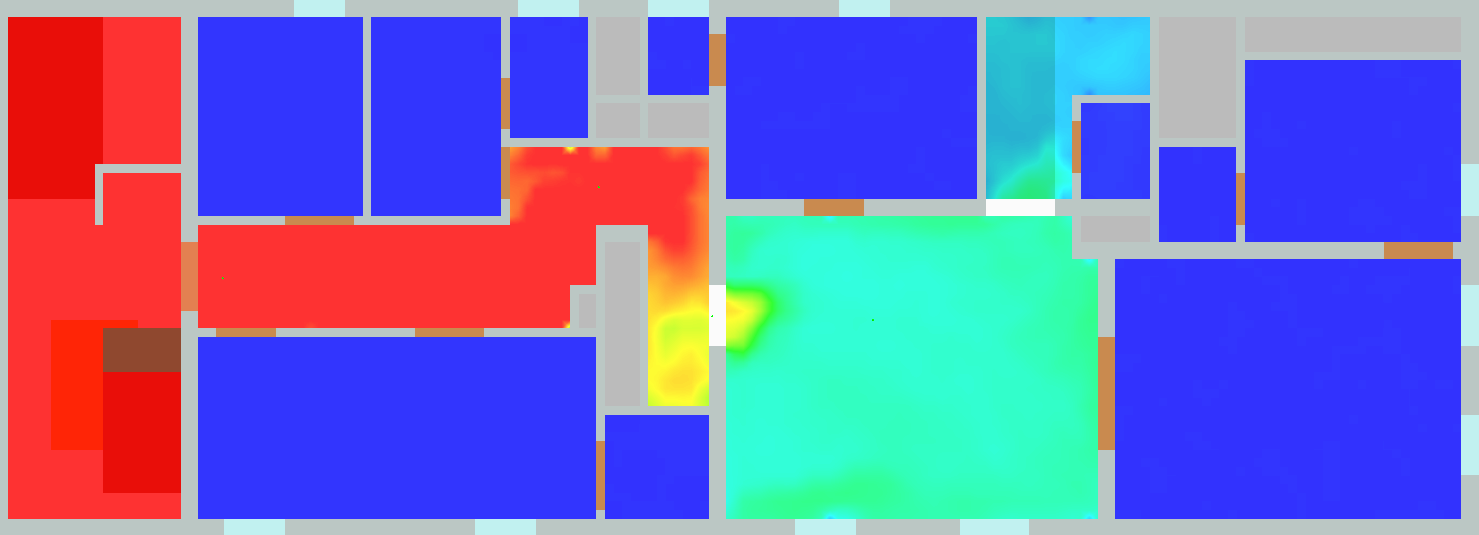
\includegraphics[width=.68\textwidth]{../Figures/west_50th_baseline_top_220_6ft}
%\documentclass{standalone}
%\usepackage{pgfplots}
%\begin{document}
%\pgfplotsset{
%	colormap={blackwhite}{[5pt]
%		rgb255(0pt)=(0,0,255); 
%		rgb255(100pt)=(0,255,255); 
%		rgb255(200pt)=(0,255,0); 
%		rgb255(300pt)=(255,255,0); 
%		rgb255(400pt)=(255,0,0)
%	},
%}
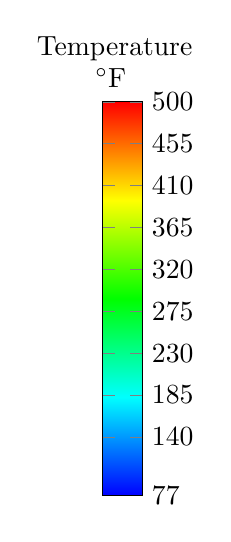
\begin{tikzpicture}
\node at (0.45,0.67) {Temperature};
\node at (0.4,0.3) {$^\circ$F};
\begin{axis}[
    hide axis,
    scale only axis,
    height=0pt,
    width=0pt,
    colorbar,
    point meta min=77,
    point meta max=500,
    colorbar style={
        height=5cm,
        ytick={77,140,185,...,500}
    }]
    \addplot [draw=none] coordinates {(0,0)};
\end{axis}
\end{tikzpicture}
%\end{document} 
%\documentclass{standalone}
%\usepackage{pgfplots}
%\begin{document}
%\pgfplotsset{
%	colormap={blackwhite}{[5pt]
%		rgb255(0pt)=(0,0,255); 
%		rgb255(100pt)=(0,255,255); 
%		rgb255(200pt)=(0,255,0); 
%		rgb255(300pt)=(255,255,0); 
%		rgb255(400pt)=(255,0,0)
%	},
%}
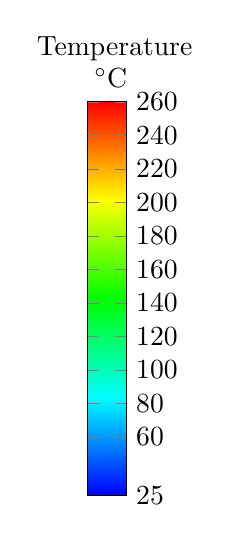
\begin{tikzpicture}
\node at (0.65,0.67) {Temperature};
\node at (0.6,0.3) {$^\circ$C};
\begin{axis}[
    hide axis,
    scale only axis,
    height=0pt,
    width=0pt,
    colorbar,
    point meta min=25,
    point meta max=260,
    colorbar style={
        height=5cm,
        ytick={25,60,80,...,260}
    }]
    \addplot [draw=none] coordinates {(0,0)};
\end{axis}
\end{tikzpicture}
%\end{document}

\caption[Temperature contours on the second floor, 60~s after interior door failure.]
{Temperature contours on the second floor, 60~s after interior door failure, 1.83~m (6~ft) above the floor.}
\label{fig:temp_top_220}
\end{figure}


\clearpage


\section{Tactical Considerations}
There have been many previous fire incidents~\cite{NIOSH:Pettit,NIOSH:Washenitz,NIOSH:Mezzanotte,NIOSH:McFall,NIOSH:McFall2,NIOSH:McFall3,NIOSH:Berardinelli,NIOSH:Koedam,NIOSH:McFall4,NIOSH:Tarley,NIOSH:Braddee,NIOSH:Merinar,NIOSH:Bowyer2,NIOSH:Loflin,NIOSH:Bowyer} in which changes in the flow paths are thought to have had an adverse impact on firefighter and occupant safety. Table~\ref{tab:lodd} lists the NIOSH investigation reports from the past 15 years in which it could be determined that a flow path played a role in the related incident. This table lists the NIOSH investigation number, the outcome, and a brief description of the flow path details.

Based on a review of these incidents, it is clear that fires with rapidly developing or changing flow paths are a significant hazard to the fire service. The development of (or changes to) a flow path could be caused by the failure of a component of the structure, such as a door, window, or portion of a ceiling, wall or floor. Environmental conditions such as wind can generate hazardous thermal conditions within a flow path. Uncoordinated ventilation can also be the cause of increased thermal hazards within a flow path. 

In this fire incident, the thermal degradation of the steel-faced, wood-framed door resulted in a rapid change in the thermal conditions in the hallway, which resulted in highly hazardous conditions. These conditions would be equivalent to or greater than a Class III exposure~\cite{Donnelly2006}. Prediction of the failure mode and failure time of the door is not a reasonable expectation given the large number of unknowns that the firefighters faced on the fire ground.  In this case, the timing of the interior attack appears to have coincided with the failure time of the door. Research has been conducted~\cite{madrzykowski2009fire, kerber2009fire} and continues to be conducted by NIST, Underwriters Laboratories (UL), and others that demonstrates that applying water from the exterior into the fire area of a structure (prior to the start of interior operations) can significantly improve the safety of firefighters by reducing the thermal hazard from the fire and reducing the potential for developing high velocity hot gas flows within the structure.

\begin{table}
\centering
\captionof{table}{Flow path related LODD/LODI incidents}\label{tab:lodd}
\begin{tabular}{lll}
\toprule[1.5pt]
NIOSH Report No. & No. of LODDs/LODIs & Flow Path Details  \\
\midrule
99-F01   \cite{NIOSH:Pettit}        &  3 LODDs            &  From apartment into hallway on 10th                  \\
                                    &                     &  floor of high-rise apartment building                \\
99-F21   \cite{NIOSH:Washenitz}     &  2 LODDs            &  Basement to 1st floor                                \\
                                    &  2 LODIs            &                                                       \\
F2000-04 \cite{NIOSH:Mezzanotte}    &  3 LODDs            &  1st floor to 2nd floor                               \\
                                    &  3 civilian deaths  &                                                       \\
F2000-16 \cite{NIOSH:McFall}        &  1 LODD             &  2nd floor hallway through                            \\
                                    &  1 LODI             &  2nd floor apartment                                  \\
                                    &  1 civilian death   &                                                       \\
F2000-23 \cite{NIOSH:McFall2}       &  1 LODD             &  From ground level to 1st floor then to               \\
                                    &  2 LODIs            &  2nd floor, flow exited through ceiling               \\
F2000-43 \cite{NIOSH:McFall3}       &  1 serious LODI     &  1st floor to 2nd floor                               \\
                                    &  2 other LODIs      &                                                       \\
F2004-02 \cite{NIOSH:Berardinelli}  &  1 LODD             &  1st floor to basement                                \\
F2005-02 \cite{NIOSH:Koedam}        &  1 LODD             &  Rear to front of the building                        \\
                                    &  4 LODIs            &                                                       \\
F2005-04 \cite{NIOSH:McFall4}       &  1 LODD             &  Basement to 1st floor                                \\
                                    &  9 LODIs            &                                                       \\
F2007-09 \cite{NIOSH:Tarley}        &  1 LODD             &  3 story training burn - flow through                 \\
                                    &  2 LODIs            &  all levels                                           \\
F2007-35 \cite{NIOSH:Braddee}       &  4 LODIs            &  1st floor to 2nd floor                               \\
F2009-11 \cite{NIOSH:Merinar}       &  2 LODDs            &  Rear to front of the building                        \\
F2011-13 \cite{NIOSH:Bowyer2}       &  2 LODDs            &  Lower level up stairs and through                    \\
                                    &                     &  entry door and garage                                \\
F2011-31 \cite{NIOSH:Loflin}        &  1 LODD             &  Fire extended from lower level apartment             \\
F2012-28 \cite{NIOSH:Bowyer}        &  1 LODD             &  Attic fire extended into closed                      \\
                                    &  1 LODI             &  porch and then into 2nd floor                        \\
\bottomrule[1.25pt]
\end{tabular}\par
\end{table}

\chapter{Summary}
NIST's Fire Dynamics Simulator was used to provide insight into the fire dynamics within a 2~\sfrac{1}{2}~story single family structure in Chicago, IL, that resulted in the death the captain of a fire department. The fuel, fire size, and fire growth rate that were used in the FDS simulations were estimated by taking into account all of the available information including the NIOSH post-incident report~\cite{NIOSH:Bowyer}, post-incident pictures, videos, and relevant literature. This resulted in a specified source fire of 12.3~MW. However, based on the limited ventilation conditions in the attic and enclosed porch, the FDS simulation results indicated a maximum HRR of approximately 9~MW as a result of the limited supply of oxygen.

The fire started in the attic and spread down into the enclosed porch on the rear of the structure. The spread of fire and hot gases into the second floor of the structure was limited by a closed steel-faced, wood-framed door that was located between the enclosed porch and the hallway. After exposure to the elevated temperatures and pressure from the fire in the porch area, the wood frame of the door decomposed and the steel faces of the door failed and collapsed inward. The door failure resulted in the establishment of a flow path between the higher pressure and higher temperature conditions in the enclosed porch and the lower pressure and lower temperature conditions in the hallway and kitchen areas of the second floor. The temperature of the gases that flowed into the hallway at face height exceeded 260~$^{\circ}$C (500~$^{\circ}$F). Unfortunately, a captain and firefighter were advancing a hose line in the hallway at the time of the door failure. The captain was overcome by the rapid change in conditions before he could exit to the safety of the kitchen area. After a Mayday call, the captain was rescued from the structure but later succumbed to his injuries.


\chapter*{Acknowledgments}
The authors would like to thank the Chicago Fire Department, especially Commissioner Jose Santiago, District Chief Donald Hroma, and District Chief Kevin Krasneck. The authors would also like to thank John Culbertson of Central Valley Fire District, MT, for his assistance in compiling Table~\ref{tab:lodd}. Finally, the authors would also like to thank Keith Stakes of NIST and Joseph Willi of the University of Illinois Urbana-Champaign for their assistance in creating the drawings of the structure.


\bibliography{../../../Bibliography/FDS_refs,../../../Bibliography/FDS_general}

\appendix

\chapter{Dimensioned Drawings}

\begin{figure}[!ht]
\centering
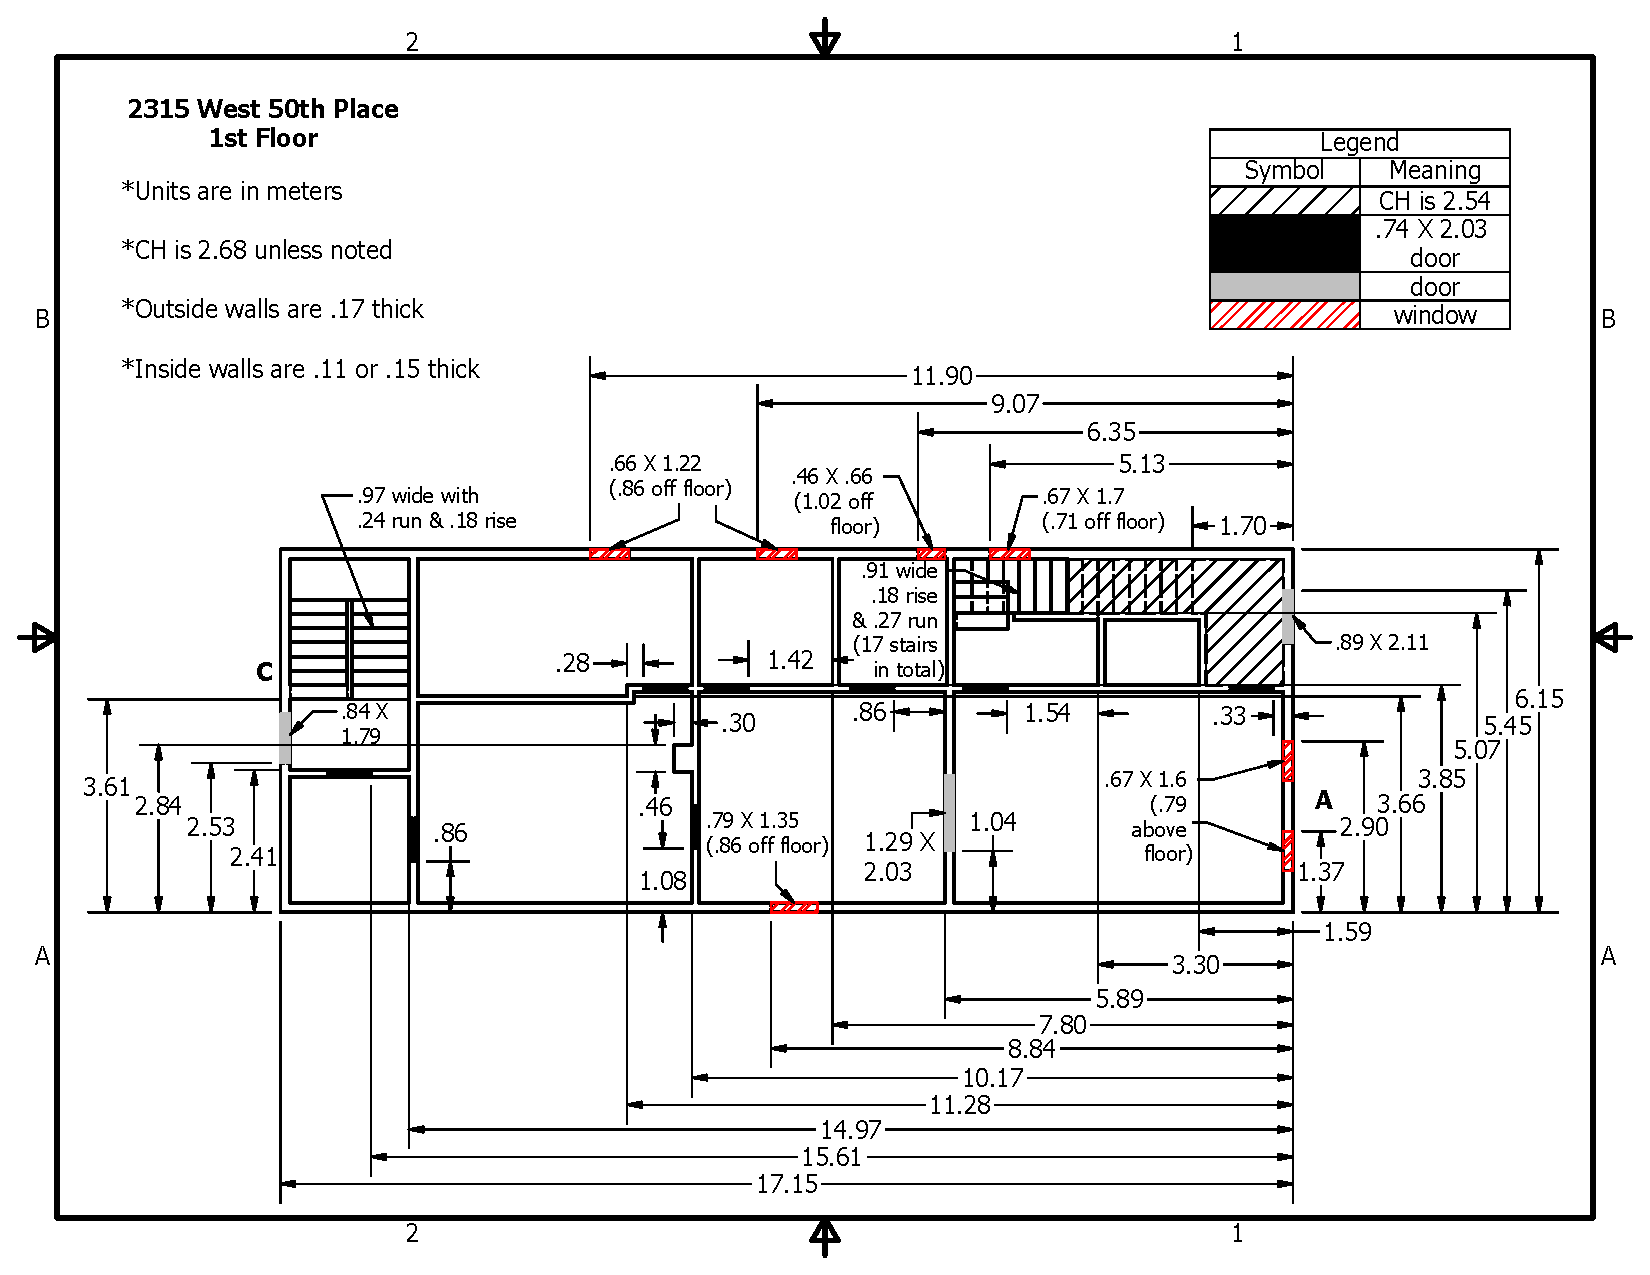
\includegraphics[width=1\textwidth]{../Figures/50th_Place_1st_Floor}
\caption[Dimensioned drawing of first floor.]{Dimensioned drawing of first floor. The measurements are accurate to within 15~cm (6~in).}
\label{fig:first_floor}
\end{figure}

\begin{figure}[!ht]
\centering
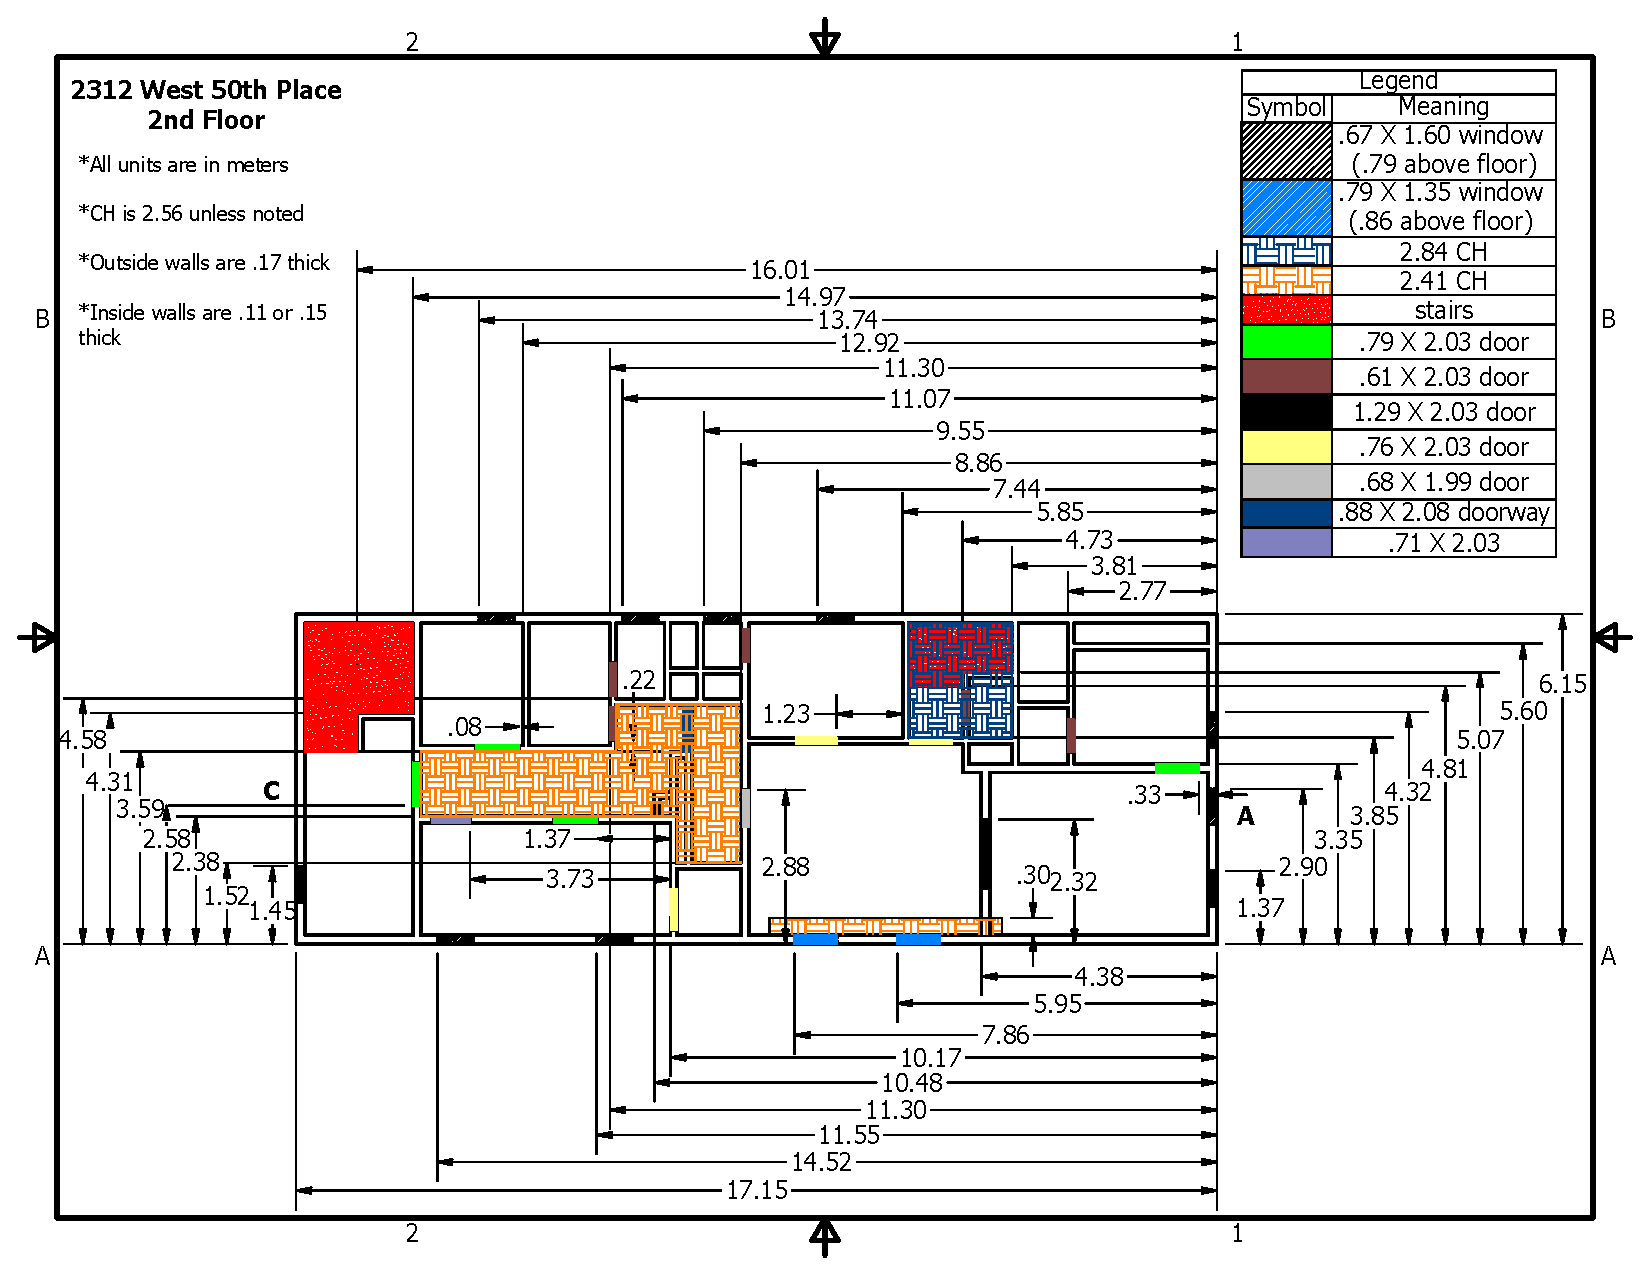
\includegraphics[width=1\textwidth]{../Figures/50th_Place_2nd_Floor}
\caption[Dimensioned drawing of second floor.]{Dimensioned drawing of second floor. The measurements are accurate to within 15~cm (6~in).}
\label{fig:second_floor}
\end{figure}


\end{document}
